\documentclass{sigchi}
% Arabic page numbers for submission. 
% Remove this line to eliminate page numbers for the camera ready copy
\pagenumbering{arabic}

% Load basic packages
\usepackage{balance}  % to better equalize the last page
\usepackage{graphics} % for EPS, load graphicx instead
\usepackage{times}    % comment if you want LaTeX's default font
\usepackage[hyphens]{url}
\usepackage{color}

\usepackage{pdflscape}
\usepackage{longtable}
\usepackage[strict]{changepage}
\usepackage{ngerman}

\usepackage{xcolor}
\newcommand\todo[1]{\textcolor{red}{#1}}

\usepackage[stretch=10,shrink=10]{microtype}

\SetExtraKerning[unit=space]
    {encoding={*}, family={bch}, series={*}, size={footnotesize,small,normalsize}}
    {\textendash={400,400}, % en-dash, add more space around it
     "28={ ,150}, % left bracket, add space from right
     "29={150, }, % right bracket, add space from left
     \textquotedblleft={ ,150}, % left quotation mark, space from right
     \textquotedblright={150, }} % right quotation mark, space from left

% llt: Define a global style for URLs, rather that the default one
\makeatletter
\def\url@leostyle{%
  \@ifundefined{selectfont}{\def\UrlFont{\sf}}{\def\UrlFont{\small\bf\ttfamily}}}
\makeatother
\urlstyle{leo}

% To make various LaTeX processors do the right thing with page size.
\def\pprw{210mm}
\def\pprh{297mm}
\special{papersize=\pprw,\pprh}
\setlength{\paperwidth}{\pprw}
\setlength{\paperheight}{\pprh}
\setlength{\pdfpagewidth}{\pprw}
\setlength{\pdfpageheight}{\pprh}

% create a shortcut to typeset table headings
\newcommand\tabhead[1]{\small\textbf{#1}}

% Make sure hyperref comes last of your loaded packages, 
% to give it a fighting chance of not being over-written, 
% since its job is to redefine many LaTeX commands.
\usepackage[pdftex]{hyperref}
\hypersetup{
pdftitle={Supporting public deliberation through spatially enhanced dialogs},
pdfauthor={LaTeX},
bookmarksnumbered,
pdfstartview={FitH},
colorlinks,
citecolor=black,
filecolor=black,
linkcolor=black,
urlcolor=black,
breaklinks=true,
}

% End of preamble. Here it comes the document.
\begin{document}

\title{Supporting public deliberation\\through spatially enhanced dialogs}
\subtitle{Master thesis}

\numberofauthors{1}
\author{
  \alignauthor Gerald Pape\\
    \affaddr{Institute for Geoinformatics}\\
    \email{\href{mailto:g.pape@uni-muenster.de}{\nolinkurl{g.pape@uni-muenster.de}}}\\
}

\maketitle

%%%%%%%%%%%%% Abstract %%%%%%%%%%%%%

\begin{abstract}
Public deliberation conducted by citizen initiatives is an important part of the democratic foundation of our society. Mostly Internet pages, meetings and newspaper advertisements are used as medium for informing the public. Giving citizens the opportunity to actively participate through discussing public matters is a step into profound deliberation. This thesis will explore the support of public deliberation performed by citizen initiatives through spatially enhanced dialogs. For this, a prototypical spatial discussion platform was developed, which will be provided to a local citizen initiative for a sustainability project. Then, semi-structured interviews, expert interviews and a focus group were performed to answer how public deliberation performed by citizen initiatives could be supported tho 


suppor could manifest itself. 


Results show some impediments but general helpfulness for supporting public deliberation performed by citizen initiatives through spatially enhanced dialogs.
\end{abstract}


This thesis features three work packages. 




%%%%%%%%%%%%% Chapters %%%%%%%%%%%%%

  \section{Introduction}
\todo{Rechtschreibung überprüfen im gesamten Dokument.. ich merke da nichts an.}
\label{chap:introduction}
Public deliberation serves the purpose to give citizens the means to educate themselves about public matters \cite{page1996deliberates}. In this context, democracy heavily relies on the ability and willingness of citizens to deliberate themselves. Deliberation is the process of considerate informing and weighing of options related to a topic. In addition to the distribution of information, every stakeholders' participation is required for a healthy relationship between citizens and their government \cite{Arnstein1969_citizen_participation}.\\
Since their first appearance, Web 2.0 applications are being used because of their collaborative character to gather information and opinions from users \cite{o2007web}. Today, modern information technologies and the Internet are ubiquitous in many aspects of daily life. Involving citizens in decision-making processes concerning public matters through such named applications and technologies led to the creation of the field ``e-Participation''. Its premise is to strengthen democratic processes between citizens and their governments through previously mentioned modern information technologies \cite{Saebo_eParticipation, Medaglia2012_eParticipation}. One of many aspects of e-Participation is public deliberation, which revolves around engaging citizens in dialogs about their surroundings and involving them in decision-making processes. In the past, these decision-making processes were performed by experts with specialized tools and domain-specific data at their respective agencies. The increasing digitization of more spatial data led to the development of spatial decision support systems (SDSS) \cite{densham_sdss}. These systems, which usually require professional training in order to be used effectively, were specifically developed to serve experts in public planning. Citizens could only participate if they attended public meetings or read notices at the departments. Subsequently, participation was limited to certain times and places.\\
Following the idea to involve citizens in decision-making processes using geographic information systems, the research field of participatory GIS was formed \cite{Macintosh2004_eParticipation_characterization,Sieber2006_PublicParticipationGIS}. Hence, the target group of spatial decision support systems shifted from experts to the general public. Participatory GIS allow citizens to partake in decision-making processes through Internet based systems. Rinner proposed the idea of ``Argumentation Maps'' \cite{Rinner_ArgumentationMaps}, which specifically foster discussions through spatial references. The idea is based on the assumption that locating arguments in a discussion spatially enhances the comprehensibility of the arguments and contributions. Since then, multiple implementations and extensions of Rinners ``Argumentation Map'' idea were developed and tested.\\
The use case of supporting decision-making processes and planning around public matters is being addressed extensively in participatory GIS research. Some of the research topics in question are user trust, representation of minorities \cite{Carver2001_PPGIS_Cyberdemocracy}, level of participation \cite{Steinmann2005_Combination_Ladder_GIS}, and prevention of information duplication \cite{Hopfer2007_Communication}. So far, research of enabling citizen initiatives through spatially enhanced dialogs has been conducted very sparsely \cite{Cai2009_spatial_annotation_deliberation}. The contribution to citizen deliberation of citizen initiatives as intermediaries between citizens and government should not be overlooked. Although some research about the use of ``new spatial media'' by citizen initiatives has been conducted \cite{Elwood2013_NewSpatialMedia}, the focus lies more on opportunities for social engagement than on participation or deliberation.\\
This thesis tries to answer the following research question:
\begin{itemize}
  \item[] \textbf{RQ:} How does the use of spatially enhanced dialogs support public deliberation performed by citizen initiatives?
\end{itemize}

Emphasis is on how explicit spatial references in discussion contributions enable citizens and citizen initiatives to discuss and deliberate about public matters. Therefore, a spatial online discussion platform was developed, which allows participants of a discussion to reference geo-locations in their contributions. Evaluation revealed that although finding the developed prototype suitable for spatially enhanced dialogs, it seems that visualizing spatial relations, and proximities is more important among citizen initiative members. It was performed among citizen initiatives members as well as domain experts of argumentation mapping and web application usability. The ability to engage in spatially enhanced dialogs about geo-features is considered a great addition, but evaluation participants feared that society will show a limited acceptance of spatially enhanced dialogs. Furthermore, citizen initiatives are discouraged with constantly managing the discussions.\\
In order to describe the research performed in this thesis, it is structured as following: \hyperref[chap:related_work]{Section 2} explores related research in the fields of participation, e-Participation and participatory GIS. The concept of the developed prototype along with application design and implementation is described in \hyperref[chap:approach]{section 3}. Furthermore, \hyperref[chap:methodology]{Section \ref{chap:methodology}} gives insight into the evaluation methods and the approach for the development of the prototype. \hyperref[chap:methodology]{Section 5} shows the findings of the three evaluation steps, while \hyperref[chap:discussion]{section 6} discusses the evaluation results, methodology and limitations of this thesis. Finally, \hyperref[chap:conclusion]{section 7} summarizes the work in this thesis and gives recommendations for future work.
% Die wollen das ding haben, aber aus den falschen Gründen. Die sehen nur die Möglichkeit damit ihre Projekte auf ner Karte sichtbar zu machen. Die haben verstanden, was spatially enhanced dialogs sind, enthusiasm ist aber definitiv auf der informing stage
  \section{Related Work}
\label{chap:related_work}
This section will explore previous research in the fields of participation, e-Participation, participatory GIS and argumentation mapping.% and evaluation techniques to provide an overview of the fields.

%\todo{Van Eemeren and Grootendorst (1996) and Tweed 1998 for definition of argumentation or discussion}
%\todo{\cite{Elwood2013_NewSpatialMedia}}


\subsection{History of Participation Research}
%%% Ladder
By defining eight levels of increasing citizen participation, Arnstein \cite{Arnstein1969_citizen_participation} coined the term ``ladder of citizen participation'' which, since then, has been adapted and modernized \cite{Connor1988_new_ladder,carver2003future,Collins2009_social_learning,you2009_participatory_map_based,Cai2009_spatial_annotation_deliberation,Macintosh2004_eParticipation_characterization,Schlossberg2005_PPGIS} by several authors. She claims that citizen participation is a term for the redistribution of power among citizen. While the first two rungs on the ladder are denoted as ``Nonparticipation'', involvement of citizens begin at the third level ``Informing''. ``Consultation'' and ``Placation'' are also labeled as ``Tokenism''. The last three steps (``Partnership'', ``Delegated Power'', ``Citizen Control'') are then declared as ``Citizen Power'' by Arnstein.\\
Structured similarly, Wiedemann and Femers \cite{Wiedemann1993355} proposed a ladder which is based on the premise that information given to the public and amount of possible participation is collateral. By requiring the implementation of the previous steps before the higher levels can be reached, Each step on their ladder leads to more and more empowerment of citizens. Wiedemann and Femers conclude that general understanding of an issue is a first step towards public participation.\\
In reaction to the ladder proposed by Arnstein, Connor \cite{Connor1988_new_ladder} constructs his version of a new ladder ``whose elements have a cumulative effect''. It is designed lead decision makers to apply techniques ``to prevent and resolve public controversy about various proposals''. %\todo{HIER NOCH WAS SCHREIBEN}

\subsection{The use of Internet communication technologies in Participation, Government and Democracy}
%%% Information of citizens
As stated by Arnstein \cite{Arnstein1969_citizen_participation}, involvement of the public begins with the supply of sufficient information. This includes the publishing of information as well as contacting officials with suggestions and questions. Traditional contacting means were transformed to use modern information technologies. Reddick \cite{Reddick2005_Citizen_interaction_with_egovernment} described this process in citizen interaction as an improvement over traditional means to contact their government. Although often lacking interaction by only serving the information needs of citizens, the Internet enables citizens to skip ``street-level bureaucrats''. The author gives the recommendations, that focus should be laid on ease of use, user friendliness and marketing of online services. Reddick also warns of digital divide by excluding non-tech savvy population groups.\\
Because contacting officials is the most common act of political participation after voting, a comparison of traditional contacting methods with Internet based contact methods was conducted by Bimber in 1999 \cite{Bimber1999_Citizen_communication_with_government}. Specifically, he tried to answer if the medium of contacting officials matters by conducting a survey with 2021 participants. He found that the Internet is ``just'' incrementing the connection between citizen and officials, not ``revolutionizing'' it.\\
A thorough review of 131 ``e-Participation'' articles was conducted by S{\ae}b{\o} et al. \cite{Saebo_eParticipation}. E-Participation is generally understood as ``joining in'', taking part or taking role and is normally associated with political deliberation or decision making. It can take place in and outside of political processes and makes use of Internet communication technologies. The work of S{\ae}b{\o} et al. was continued by Medaglia in 2012 \cite{Medaglia2012_eParticipation}. He reviewed 122 e-Participation articles published between 2006 and 2011. Both S{\ae}b{\o} et al. and Medaglia classify the e-Participation research domain using the categories ``Actors`` which conduct ``Activities'', ``Effects'' which are the results of ``Activities'', ``Activities'' influence on other ``Activities'' and ``Evaluation'' of ``Effects' which improve the ``Activities''. Susha et al. \cite{Susha2012_eParticipation} found an analogue classification of e-Participation research. Their categories are ``stakeholders'', ``environment'' and ``applications and tools''.\\
In 2004, Macintosh \cite{Macintosh2004_eParticipation_characterization} defined ``e-Democracy'' as ``the use of Internet communication technologies to support the democratic decision-making processes''. In order to better understand this definition, she described several key dimensions of e-Participation. Analogous to the participation ladders of Arnstein, Wiedemann and Connor \cite{Arnstein1969_citizen_participation,Wiedemann1993355,Connor1988_new_ladder}, the level of participation is one of these key dimensions. Additionally, the stage of policy-making in which the citizens are engaged should be considered carefully according to Macintosh. Who should be engaged by whom, technologies used, rules and duration of engagement are other important key dimensions. Finally, evaluation and outcomes should be reflected thoroughly.\\
Above the one-directional ``Informing'' stage lies the bilateral communication in form of discussions and dialogs which also serves as base for the so called ``e-Participation'', ``e-Government'' and ``e-Democracy''. Kent and Taylor proposed a theoretical framework for building dialogic relationships through the Internet in 1998 \cite{Kent1998_dialogic_relationships_through_www}. In their understanding, dialogic communication is ``any negotiated exchange of ideas and opinions''. Participants in a dialog not necessarily have to agree, but are in it to reach a mutually satisfying position. Dialog is about creating shared subjective views and focuses on the attitude towards each other. The Internet aids this process by allowing both synchronous and asynchronous means of communication.\\
A three step procedure to apply and organize public participation above the ``Informing'' stage was proposed by Renn et al. in 1993 \cite{Renn1993_participation}. Values and concerns of citizens and stakeholders are structured into an hierarchy which then are discussed and judged by experts. The results are then evaluated in citizen panels. Participants can be divided into three groups. Stakeholders which bring concerns and interests, as well as metrics for evaluation. Experts serve as base for related data and to uncover functional relationships between options and their impacts. Finally, citizens, as potential victims and benefactors, assess the results and outcomes of the proposals of the other groups.\\
Online forums as a tool for mass deliberation were evaluated by Wright and Street \cite{Wright2007_deliberation_design}. They found, that current online forums are not designed for social interaction. Furthermore, both proponents and opponents of mass deliberation through online forums miss the role played by design in facilitating or thwarting deliberation and tend to tread information technology as given and determinant. Wright and Street conclude that technology is both shaped by and shaping political discussion on the Internet and recommend to focus on moderation of discussions in online forums.\\
Jaeger \cite{Jaeger2005_deliberate_democracy_and_egovernment} explored potential social impediments of the increasing use of Internet communication technologies in e-Government and e-Participation. Through survey of existing information studies in public policy, law and governance, he found that the Internet ``poses real dangers of creating or fostering social fragmentation''. Through the asynchronous nature of interaction, avoiding people with contrary opinions and finding people with same opinions is easier than in real world situations, like a public hearing. Set-ups like these tend to facilitate group polarization. Jaeger states, that members of such groups with shared beliefs or shared identity are more likely to tend to extreme opinions. Anonymity of Internet-discussions further increases tendencies to take extreme positions. Apart from these concerns, he clearly sees an advantage in applying Internet communication technologies and ``could could potentially benefit the health of the entire democracy''.\\
Public deliberation through decision support with pro/con lists were evaluated by Kriplean et al. \cite{Kriplean2012_Considerit}. Their system allows to create public pro/con lists in which other participants pro/con points could be included. The lists then created an overview of all stances and contributions. This indirect discussion mitigates ``political identity and flaming'' by forcing the users to reflect on their standpoints and disallowing any portrayal of political affiliations.\\
In 2009, Collins and Ison \cite{Collins2009_social_learning} suggested that the traditional ladders of Arnstein and colleagues are too dominating in citizen participation in policy discourses. They propose to focus more on the social learning aspect of participation which builds upon convergence of goals, co-creation of knowledge and change of behavior and actions. If all participants and stakeholders apply this ``social learning'', understanding is supported.%\todo{mehr!}

\subsection{Geographic information systems in decision making and argumentation}
\label{subchap:gis_stuff}
As early as the development of geographic information systems (GIS), they were used to support experts in making decisions. An early overview over spatial decision support systems (SDSS) is made by Densham in 1991 \cite{densham_sdss}. Standard decision support systems were developed to support experts in solving ``ill-structured'' problems where the definition of problem is difficult. By combining existing data with statistical models, solution space can be explored. The ability to weigh the different factors, multiple decision-making styles are supported. The introduction of spatial capabilities into an decision support systems brings several benefits and allow to solve semi-structured spatial problems. Additional features of spatial decision support systems are the ability to store and illustrate spatial relations, the analysis through statistical methods and to create maps as output. Densham proposes a ``SDSS generator'' for future development which combines analysis tools, GIS functionalities and database management systems. Furthermore, the differentiation between ``Objective'' and ``Map'' space is deemed important. Users must be able to view both spaces simultaneously, which update each other when changes are made to either one.\\
Following the developments in spatial decision support systems, the concept of Public Participatory GIS (PPGIS) and Participatory GIS (PGIS) emerged. Both focus on enabling non-expert groups to apply GIS technologies to strengthen involvement in decision making.\\
In 2006, Sieber \cite{Sieber2006_PublicParticipationGIS} traces the social history of PPGIS and lists mayor themes found in PPGIS research. ``Place and People'' relate to the question ``who should be participating in PPGIS projects''. ``Technology and Data'' cover representation of knowledge, accessibility of data and appropriateness of information. ``Process'' focuses on descision-making structures and processes, participation and communication in the policy making process and system implementation and sustainability. The ``Outcomes and Evaluation'' measures goals and results. The themes are similar and related to Macintosh's \cite{Macintosh2004_eParticipation_characterization} key dimensions of eDemocracy. Sieber also notes that, although PPGIS have been constructed and practised by a broad set of actors in multiple research disciplines, GIS alone is controversially attributed to enhance public participation and deliberation. Similar observations were made by Obermeyer \cite{obermeyer1998evolution}, Craig et al. \cite{Weiner2002_Participation_and_GIS_eigentlich_Craig} and Blaschke \cite{Blaschke2004_PGIS_critically_revised}. According to Blaschke, broad participation of the public is the distinction of PPGIS from SDSS. He also claims that public participation does not automatically lead to better decisions.\\
Schlossberg and Shuford tried to delineate the terms ``public'' and ``participation'' in PPGIS through a literature review \cite{Schlossberg2005_PPGIS}. They defined a matrix with ``Domain of Participation'' and ``Domain of Public'' as axes. The ``Domain of Participation'' axis contains participation techniques which the actors on the ``Domain of Public'' axis perform. The axes are ordered from simple to complex. The ``Domain of Participation'' dimension is leaned against the various participation ladders defined by Arnstein and colleagues \cite{Arnstein1969_citizen_participation,Wiedemann1993355,Connor1988_new_ladder}. They populate their matrix with four scenarios.\\
Voss et al. \cite{Voss2004_Evolution_PGIS} describe the combination of a structured argumentation tool, Dito and a spatial decision support system, CommonGIS. The integration of the systems was made gradually over the course of three experiments exploring different aspects of spatial discussions. Through these, they identified multiple conceptual, technical and user interface requirements. Due to their approach to combine two existing systems, several technical issues emerged.\\
Alongside with an overview of PGIS systems, Jankowski \cite{Jankowski2005_community_based_pgis} analyzes two studies in PGIS water resource decision making. In both cases, participants had to make suggestions for water source protection sites. The second case featured shared displays for the conveying of spatial data. Jankowski found that trust in state supplied data were not high and that the technology sometimes reduced creativity, especially if it was hard to use. He also finds that citizens need to have real interest and insight in information in order to support decisions effectively. Future systems should focus on how technology can be used without reducing the creativity of participants.\\
Rinner \cite{Rinner_ArgumentationMaps} picked up on the idea of PPGIS but focused on he combination of e-Participation principles (use of Internet communication technologies to involve citizens in discussions about decision processes) with geographic information systems. After a review of discussion and collaboration tools, he found that asynchronous discussions were not considered during planning procedures. Following this, Rinner proposed the concept of ``Argumentation mapping''. He described four use cases which outline the design of argumentation mapping. The GIS functionality of spatial data presentation is used for navigation in argumentation maps. Similar to Goodchild's concept of volunteered geographic information \cite{goodchild2007citizens}, Rinner translates input of geographic data to participation. Retrieval and analysis functions of GIS can be used for exploration and evaluation in argumentation maps. These use cases can only be used fully, if an object-based model of geographically referenced argumentation is used.\\
Since then, multiple implementations of argumentation mapping and PPGIS systems with multiple research goals and outcomes have emerged.\\
In 1999, Kingston et al. \cite{kingston1999gis} developed a PPGIS system to enable a digital version of annotated map pins. The system allowed to create comments with a spatial reference. It lacked a structured discussion support and allowed only one spatial reference per comment.\\
Multi-criteria evaluation (MCE) is a computation method to bring alternative solutions of a problem into an order by applying metrics to the different parameters of the problem. MCE is seen as an alternative to ``hard'' boolean filters used in SDSS. In order to answer if geovisualization in multi-criteria evaluations can support spatial decision making, Rinner \cite{Rinner2007_geovis_decisionsupport} conducted two studies where users could evaluate different outcomes of a problem by manipulating parameters with sliders. The result of the parameter manipulation was immediately visible on both a map and diagrams. Rinner found, that his solution with sliders suppported the decision making process.\\
A first implementation of the argumentation map idea was made by Ke{\ss}ler et al. \cite{Kessler2005_ArgumentationMapPrototype}. He proposes a set of requirements and design guidelines for argumentation maps and analyzes different options for linking maps and discussion contributions. The implementation should address the two main issues of the analyzed systems, user friendliness and support of open standards. Ke{\ss}ler's implementation featured separate discussion and map components, to which he established the requirements ``Integrated user interface'' for both components, ``Structured discussion'' in the discussion component, ``Common (Web)mapping functions'' for the map component, ``Integrated database, many-to-many relationships'' for both components and ``Access control, security'' and ``Customization by Provider'' for the discussion and map component respectively. An important aspect is the throughout use of open standards to ensure reusability. The system allowed users to upload ESRI shapefiles \footnote{\url{http://www.esri.com/library/whitepapers/pdfs/shapefile.pdf}} and create point features in a map. These spatial features could be annotated with texts and labels. An evaluation of the Argumentation map prototype implemented by Ke{\ss}ler et al. with HCI principles was then conducted by Sidlar and Rinner \cite{sidlar_argumap_2007}. They specifically investigated learnability, memorability and user satisfaction. The participants of the study were engaged about planning ideas at the University of Toronto. The questionnaires at the beginning and end of the trial periods yielded generally positive results. A list of recommendations for improvements were given by Sidlar and Rinner. They also conducted an utility assessment \cite{Sidlar2009-AssessmentMapGeocollaborationTool} of the Argumentation Map prototype. They authors state that the utility of application is often seen as given, thus developed a framework for investigating participatory GIS utility. Utility was measured by calculating ratios of actual use of argumentation mapping functions over the potential us of those functions. After applying their framework to the prototype in a study, Sidlar and Rinner reached to the conclusion that every aspect of the Argumentation map prototype was used but ``not always to its fullest''.\\
A combination of a spatial data infrastructure as extension to the Argumentation map prototype from 2005 is discussed by Ke{\ss}ler et al. \cite{Kessler2005_Conflict_Resolution}. As PPGIS applications naturally make extensive use of geographic information, the authors argue that participatory discussions in PPGIS could benefit from readily available geospatial data. They also implemented basic analysis functionalities and applied their idea in a conflict resolution context. Ke{\ss}ler et al found that spatial data infrastructures can ease and simplify the setup of a PPGIS as geospatial objects to discuss are readily available.\\
Two systems in PPGIS context were developed by Carver et al. \cite{Carver2001_PPGIS_Cyberdemocracy} to find out how the Internet and GIS can be used together in order to provide the public with becoming more involved in environmental decisions. While the first system only conveyed information about a natural reserve, the other was used for collecting citizen ideas to improve a small town. They identified technological issues with implications for decisions with citizen involvement. Although access to geospatial (and nongeospatial) data and tools may empower the general public to contribute to decision processes, participation is held back by inequalities of citizens in their computer literacy. The authors also list principles for future implementations of web based PPGIS applications.\\
In their article ``Design of a GIS Enabled Online Discussion Forum for Participatory Planning'' Tang et al. focus on effective communication and mutual understanding \cite{Tang2005_PPGIS_discussion_forum}. They reviewed eleven PPGIS applications for participatory planning. Among these eleven were systems of Carver \cite{Carver2001_PPGIS_Cyberdemocracy} and Rinner \cite{Rinner_ArgumentationMaps}. The eleven PPGIS application were evaluated for the following criteria: Experts should be able to play the facilitators role, exchange of views must be supported as well as the documentation and sharing of the evolution of ideas, made decisions should be shown in the context of the related decisions and effectiveness of communication about spatial context. The authors revealed several shortcomings of the reviewed applications and discussed the development of GeoDF. Being the co-authors of Tang et al. \cite{Tang2005_PPGIS_discussion_forum} Zhao and Coleman \cite{zhao2006geodf} summarize the process and lessons learned in implementing the GeoDF prototype which is a GIS-enabled online discussion forum to enable citizens of a small town in Canada to provide in-depth feedback to the government. Textual components and spatial context have a one to one relationship. The spatial context consists of map extent, visible layers, annotations and sketches from both the contributor and other contributors. Due to the use of proprietary technology, issues of data availability, licensing, maintenance, re-usability and interoperability emerged.\\
The development of a multi-criteria decision support system in combination with an argumentation map is described by Sim\~{a}o et al. \cite{Simao2009Webbased}. They used their system to educate their users about all outcomes of a collaborative planning process. Their application consists of a three tier architecture which the users are navigated through. After an information area, the actual MC-SDSS (multi-criteria spatial decision support system) is entered where the solution space could be explored. The last step is a map centric communication tool to record opinions about the explored solutions. Finally, most discussed solutions are assessed by experts. During the development, the authors identified problems of planning processes. Often the problems have many dimensions, making the definition of the problem statement beforehand really difficult. As well as expert knowledge, communication is key in finding the best solution.\\
The use of Web 2.0 principles and technologies for collaborative spatial decision-making was assessed by \cite{Rinner2009_Web2_argumap} et al. by re-implementing the original Argumentation map by Ke{\ss}ler \cite{Kessler2005_ArgumentationMapPrototype} called ``ArgooMap''. It allows users to submit place based comments and to respond to other comments. Only marker as spatial reference were allowed. The authors evaluated their thread based online map discussion forum with a simulation. Existing discussions were re-enacted in a sandbox with no user interaction.\\
An implementation of a multi-criteria decision analysis (MCDA) tool was described by Boroushaki and Malczewski \cite{Boroushaki2010_ParticipatoryGIS}. They took the ArgooMap prototype of Rinner et al. \cite{Rinner2009_Web2_argumap} and extended it by adding multi-criteria decision support. Automatically generated problem solution alternatives could be discussed through the ArgooMap part. A follow up paper of Boroushaki and Malczewski evaluated their MCDA implementation through a study with citizens \cite{Boroushaki2010_Consensus_measurement}. They identified bringing together experts and laypeople as a main challenge of GIS-based spatial decision-making tools. The goal should always be to reach a high consensus among decision-makers and citizens. Another evaluation of the MCDA implementation of Boroushaki and Malczewski was conducted by Meng and Malczewski \cite{Meng2010_ArgooMap_evaluation}. They tested the usability of the front end ArgooMap with a user study where participants had to choose and discuss possible parking facility sites. They measured usability through perceived user effectiveness, efficiency and satisfaction. They found that effectiveness has a strong influence on how long a user stays on the website and efficiency impacts on user visit numbers, page views and interaction with others. Meng and Malczewski suggested that user testing should be considered in system-design processes of web-PPGIS.\\
 General concepts and methods for designing Web 2.0 community-based geoportals are presented by Longueville \cite{Longueville2010_community_based_geoportals_web20}. He sees community-based geoportals as advanced spatial data infrastructures which should allow users to gather and share resources, organize themselves into groups and to create resources collaboratively. Each resource should also include meta-resources like popularity, tags and comments. Longueville recommends to modularize applications to create both human and machine readable interfaces.\\
Cherubini and Dillenbourg \cite{Cherubini2007_shared_maps} tested a chat system that allows its users to create spatial references either through displaying the chat contributions directly on a map or referencing map features through symbols in the text. They found in an user study, that the references provided a tool to reinforce the reference frame of the conversation. Also, the explicit referencing made communication more efficient. Participants used fewer sentences with fewer words. Hopfer and MacEachren \cite{Hopfer2007_Communication} applied a group communication theory, the Collective Information Sharing (CIS) bias, to a geospatial annotation tool. The authors found that the ability to annotate map-based displays can ease spatial communication tasks and enables participants of a discussion to move beyond ``what are we talking about'' to ``who knows what about an area and how this could be of use''. Therefore visualizing all information spatially will enable users to see gaps and thoroughly covered areas and reduce repeat of known information. ``Information that is made visually explicit is more likely to be recalled and, therefore, discussed''. The authors give design recommendations in applying CIS to the design of a geospatial collaboration tool. Cai and Yu \cite{Cai2009_spatial_annotation_deliberation} discuss the challenges of spatially enabled public deliberation. In their opinion, PPGIS brings together the analytical capabilities of GIS with deliberative capabilities of discussion forums. They distinguish two deliberation types, cognitive and practical deliberation. Similarly to Arnsteins' ladder, they define five phases of geodeliberative dialogs. After a stage of ``Briefing and introduction'', geodeliberative dialogs' purpose is to ``Elaborate on problems and issues''. Next it allows to ``Contribute personal knowledge, experiences, and stories'', which then aids ``Development of public judgment and creation of a common ground''. The final stage is comprised of ``Generating and evaluating alternative courses of actions''.\\
A set of non-functional requirements of scalable, reliable and easy-to-maintain applications in a cloud computing context are given by Sani and Rinner \cite{Sani2011_Scalable_Argumap}. They state that system security, performance and scalability, robustness, availability and fault tolerance, maintainability and portability, modifiability and testability are the key non-functional requirements when developing a scalable argumentation mapping tool.\\
Although described in their respective literature, very few systems are readily available for an examination of their functionality and mode of operation. However, there are several civic implementations of spatially enhanced discussion tools in existence.\\
The project nexthamburg\footnote{\url{http://www.nexthamburg.de/}, Kulus et al. \cite{Kulus_nexthamburg}} enabled citizens of Hamburg to suggest ideas for its urban development. The ideas were located on a map and other citizen could comment on the suggestions and ideas. Experts and decision makers then evaluated the ideas to implement them. The concept spawned a similar project in Kassel\footnote{\url{http://www.nextkassel.de/}}. The suggestions and ideas are only loosely tied to a location.\\
The ``Shareabouts''\footnote{\url{http://openplans.org/shareabouts/}} and ``CollaborativeMap.org''\footnote{\url{http://www.collaborativemap.org/home/}} applications use a spatial approach for gathering input of citizens. Although contributions are directly related to a spatial location, only one location per suggestions can be referred to.

%\subsection{Evaluation Methodology}
%This sub-section will explore the 
%Usability of PPGIS Haklay and Tobón \cite{Haklay2003_ppgis_usability_evaluation}


 %\cite{Pocewicz2012_Paper_vs_PPGIS} \cite{Aggett2006_evaluation_dss_ppgis}
 %\cite{Damianos1999_evaluation_collaborative}
 
%semi-structured Interviews: 
%\cite{helfferich2005} Transcription rules: \cite{kuckartz2007}  
%Focus group conduction: 
%\cite{asbury1995overview} 
    %What is a focus group: \cite{carey1994capturing} 
%\cite{morgan1996_focus_groups}

  \section{Approach}
\label{chap:approach}

As seen in \hyperref[chap:related_work]{section \ref{chap:related_work}}, research proposes various theoretical frameworks and implementations in the area of argumentation mapping. This section introduces the concept of ``DialogMap'' and gives information about the context and background of the developed prototype (sub-section \ref{sub:dialogmap}), describes general concepts of the implemented prototype (\hyperref[sub:design]{sub-section \ref{sub:design}}) and lay out implementation details (\hyperref[sub:implementation]{sub-section \ref{sub:implementation}}).

\subsection{DialogMap}
\label{sub:dialogmap}

Following the concept of Rinner's Argumentation Map \cite{Rinner_ArgumentationMaps} and the idea of supporting public deliberation through spatially enhanced dialogs, the concept of DialogMap was developed. Following the recommendations and suggestions of the research presented in \hyperref[subchap:gis_stuff]{section \ref{subchap:gis_stuff}}, a set of functional and non-functional requirements have been derived.\\
DialogMap is a spatial online discussion platform to support geodeliberative dialogs perfomed by citizen initatives \cite{Cai2009_spatial_annotation_deliberation}. It enables its users to make explicit spatial references in their discussion contributions to clarify denotation of spatial relationships. This is achieved by allowing the interlinking of one or multiple words with a location or area on the map of the application \cite{Rinner_ArgumentationMaps}. It is possible to create multiple connections between locations in one contribution, as well as referring to locations created in the context of another contribution \cite{Kessler2005_ArgumentationMapPrototype,Voss2004_Evolution_PGIS,you2009_participatory_map_based,Cai2009_spatial_annotation_deliberation} to allow more fine grained references. This creates the possibility for many-to-many connections between locations and words. It is also possible to create multiple hyperlinks on words or multiple words in the contributions' text. The creation of the references and the text can occur in any order \cite{Voss2004_Evolution_PGIS}. It was found that through allowing spatial references, exchange of information can be made more efficient \cite{Cherubini2007_shared_maps}.\\
Contributions comprise not only of a text with spatial references and hyperlinks, but is composed of multiple other attributes and properties \cite{Longueville2010_community_based_geoportals_web20,Kessler2005_ArgumentationMapPrototype,Kessler2005_Conflict_Resolution}. Users are able to specify tags and a category and to attach an image to each contribution \cite{Tang2005_PPGIS_discussion_forum,zhao2006geodf,you2009_participatory_map_based,Cai2009_spatial_annotation_deliberation} to support their statements in their contributions. The tags and category of the contribution affect the visual appearance of the geo-features created in its context.\\
DialogMap favors linear dialogs by structuring the contributions chronologically \cite{Cherubini2007_shared_maps,you2009_participatory_map_based}. Contributions can be made without context or as a reply to a contribution. It is possible to edit contributions along with its properties and created references. It is also possible to mark contributions as deleted, which results in a visual marking of the textual representation as well as the fading of the geo-features created in the context of the contribution \cite{Hopfer2007_Communication}. This further supports the linearity of the structured discussions.\\
Creation of contributions is only allowed after authenticating to the system. Users can either register an user account with a e-mail password combination or authenticate themselves through a third party authentication provider \cite{Sani2011_Scalable_Argumap,chun2014usability}.\\
The user interface of DialogMap features a map and an area to display the textual representations of a contribution. Spatial and textual representations of the contributions are interlinked by a two way highlighting to indicate the relationships between geo-features and contributions \cite{Cai2009_spatial_annotation_deliberation,Sidlar2009-AssessmentMapGeocollaborationTool}.\\
DialogMap allows to filter and search for contributions by categories, tags and by free text. This enables users to create their own contribution overviews \cite{Voss2004_Evolution_PGIS,you2009_participatory_map_based}, and allows users to see gaps and thoroughly covered areas \cite{Hopfer2007_Communication}.\\
The importance of an easy user interface was mentioned by many authors \cite{Rinner2009_Web2_argumap,Jankowski2005_community_based_pgis,Tang2005_PPGIS_discussion_forum,zhao2006geodf,you2009_participatory_map_based}. As users are likely non-technical \cite{Cai2009_spatial_annotation_deliberation}, the user interface should not discriminate them, thus suppressing participation \cite{Carver2001_PPGIS_Cyberdemocracy}.\\
An important technical aspect of the conception and development of an spatial discussion platform is to plan it flexible enough to be reused for multiple use cases \cite{Kessler2005_Conflict_Resolution,Kessler2005_ArgumentationMapPrototype,Sani2011_Scalable_Argumap}. This was adequately honored through the Model-view-controller pattern in both the backend and frontend. Another recommendation was, to make the architecture modular, to make the application scalable \cite{Sani2011_Scalable_Argumap} to serve many users at the same time.

In order to test the initial idea of supporting public deliberation through spatially enhanced dialogues, a working prototype was developed. Starting from the concept of DialogMap, a first prototypical application was developed. The development was done in an iterative and agile approach. The creation of working iterations of the DialogMap concept made early feedback possible. The possibility to evaluate the concept in a real world use case with users of scientific citizen initiatives presented itself early in the development process. The further development was then conducted with with practical advice from members of one scientific citizens' initiative. Their input ranged from general suggestions to opinions of specific features. Thus, the following sections describe the distinct outcome of their input to the developed prototype.

%``Integrated user interface'', ``Structured discussion'', ``Common (Web)mapping functions'', ``Integrated database, many-to-many relationships'', ``Access control, security'' and ``Customization by Provider''. \cite{Kessler2005_ArgumentationMapPrototype}

%Recommendations for implementing PPGIS \cite{Carver2001_PPGIS_Cyberdemocracy} \cite{Voss2004_Evolution_PGIS}

\subsection{Application Design} % and features
\label{sub:design}

Internally, the prototype uses few data models. In the configuration used for this thesis, a contribution contains a title, description, two categories, a tags field, a favored counter, an optional time restriction field for start and ending times, an optional image, an optional reference to a parent contribution and optional references to child contributions. The parent and child contribution references create a simple parent-child connection between contributions, as children inherit the categories, tags, time restriction and title. A contribution serves both as a topic and as response to a topic. A contribution also contains references to features, references to feature references and references to URLs.\\
Features are geospatial entities with a location, a reference to its contribution and properties for styling\footnote{\url{https://github.com/mapbox/simplestyle-spec}}.\\
Feature references contain a title, which can differ from the original title of the feature and a reference to a feature. URL references contain hyperlinks and a description of the hyperlink. The description of a contribution contains the text typed by a user with specially encoded references to features, URL references and feature references. Additionally, each contribution stores the ids of the users who favored it.\\
Users can create contributions in the manner of creating topics or writing responses to existing topics. Users have an e-mail address and a name. \hyperref[fig:data_structure]{Figure \ref{fig:data_structure}} depicts a generalized data structure diagram.

\begin{figure}[!h]
    \centering
    \includegraphics[width=1\columnwidth]{images/data_structure}
    \caption{Schema of the underlying data structure of the prototype. Time and id fields are omitted for brevity.}
    \label{fig:data_structure}
\end{figure}

The front page of the prototype consists of a map with a sidebar. This allows the user to see both the spatial and textual representations of a contribution at one glance. The right hand sidebar contains the input form for new contributions, filter options, sorting order selector and the list of contributions. The input form consists of input fields for title, categories, time restriction, image and description. The description field allows the creation of spatial features and URL/feature references through connecting words with spatial representations or URLs. (See \hyperref[fig:screenshot_create]{Figure \ref{fig:screenshot_create}})\\
A text area for arbitrary text and multiple checkboxes allow to restrict the listed contribution as well as the geo-features displayed in the map. It is also possible to change the sorting order of the list of contribution through a drop down field. \hyperref[fig:screenshot_filter]{Figure \ref{fig:screenshot_filter}} depicts the expanded filter with several checkboxes enabled.

\begin{figure}[!h]
    \centering
    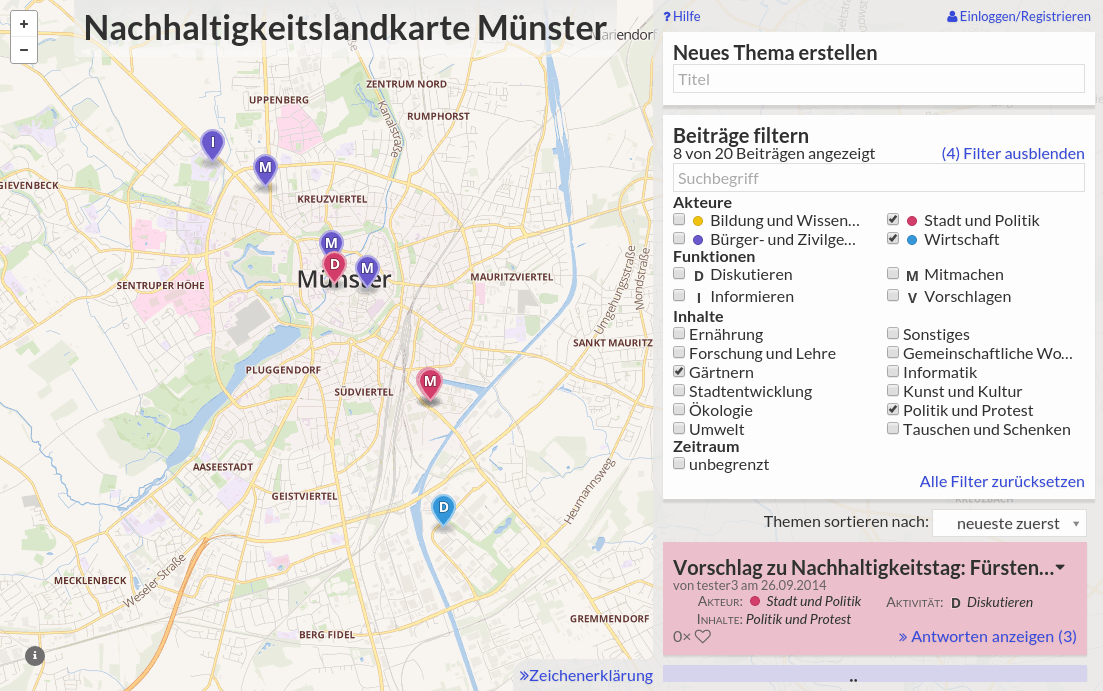
\includegraphics[width=1\columnwidth]{images/screenshot_filters}
    \caption{\textit{DialogMap} with expanded filter.}
    \label{fig:screenshot_filter}
\end{figure}

The list of contributions contains colored rectangles representing the different topics. Each rectangle contains the title, time of writing, name of the author, categories, tags and the amount of times the contribution has been favored by users. It also contains a link which navigates to the replies written to the topic. A click on the contribution rectangle expands it vertically, revealing the description of the current topic.\\
After clicking the ``reply'' link, only the selected topic and replies are shown in the sidebar in a chronological order. In this view, each contribution shows the description by default as well as author and time and date of writing. The author of the contribution is able to edit and delete the contribution. Upon deletion, the user can enter a reason for deletion, which then will be displayed below the deleted contribution. The deletion is not destructive. The contribution as well as features created for the contribution are marked visually as deleted. Other users are able to favor contribution to show interest or agreement.

\begin{figure}[!h]
    \centering
    \includegraphics[width=1\columnwidth]{images/screenshot_create}
    \caption{Input form of \textit{DialogMap} for creating a new topic.}
    \label{fig:screenshot_create}
\end{figure}

The map view contains a base map and several markers and polygons in different colors and different icons in case of markers. These relate to the contributions and are connected through the references in the description of the contributions. Which spatial features are displayed is determined through the state of the sidebar. In the topics overview, only the features created for the starting contributions are displayed in order to prevent cluttering of the view-port. When only a topic and its replies are displayed in the sidebar, all features related to the topic and its replies are shown on the map.\\
To emphasize the relationship between a contribution and its spatial features, a two way highlighting has been implemented. Hovering over either a contribution-box, marked word or spatial feature on the map triggers visual highlighting on all related contributions, marked words and spatial features. This allows to quickly grasp the relationship between features and contributions. \hyperref[fig:screenshot]{Figure \ref{fig:screenshot}} shows an active highlighting initiated through a mouseover over a marker.\\
Users are able to use either traditional sing-up/sign-in methods or sign-in through different social log-in providers to authenticate to the system.

\begin{figure}[!h]
    \centering
    \includegraphics[width=1\columnwidth]{images/screenshot}
    \caption{Screenshot of the front page of \textit{DialogMap} with active highlight of a contribution and spatial feature.}
    \label{fig:screenshot}
\end{figure}

\subsection{Implementation}
\label{sub:implementation}
\textit{DialogMap} has been implemented as a single-page web application using AngularJS\footnote{\url{http://angularjs.org/}} and Ruby on Rails\footnote{\url{http://rubyonrails.org/}}. The single-page structure was chosen in order to provide the user with a clear navigation between the overview and contribution answers. This also allows for a seamless browsing experience without full reloads of the page. AngularJS is a JavaScript framework with features like templating, two-way binding and DOM manipulation. It follows the model-view-controller pattern in order to bring server side paradigms to client-side development. AngularJS was chosen because of its popularity, extensibility and high number of available libraries. It also enables to wrap existing JavaScript libraries to be used in AngularJS context.\\
The mapping library Leaflet\footnote{\url{http://leafletjs.com/}} serves as base for displaying base maps and geospatial data. The user-facing web page was developed using tools like CoffeeScript\footnote{\url{http://coffeescript.org/}}, Haml\footnote{\url{http://haml.info/}} and Sass\footnote{\url{http://sass-lang.com/}} to speed up the development. The web page was developed with all major browsers in mind.\\
On the server side, components were developed using the Ruby on Rails framework with PostgreSQL\footnote{\url{http://www.postgresql.org/}}/PostGIS\footnote{\url{http://postgis.net/}} as data storage. Ruby on Rails, originally a full-stack model-view-controller web framework, is used as a JSON serving application logic. It was chosen because of its maturity and high number of available libraries. Front- and backend of the prototype communicate in REST-API\footnote{Representational State Transfer Application programming interface} like manner. This allows for easily replaceable front- and backend application stacks.\\
Figure \ref{fig:screenshot} shows the front page of the prototype with an active two way highlight.\\
Without the extensive use of open source software and code, development would have taken much longer. The source code as well as installation instructions are accessible online through GitHub\footnote{\url{https://github.com/ubergesundheit/dialogmap}}.





  \section{Methodology}
\label{chap:methodology}
This section will give insight into the development process of the DialogMap concept and the evaluation techniques chosen (\hyperref[subchap:ev_methodology]{section \ref{subchap:ev_methodology}}).

\subsection{Development Methodology}
As already stated in \hyperref[sub:dialogmap]{section \ref{sub:dialogmap}}, the development of the DialogMap prototype was performed in an agile and iterative manner, meaning that working prototypes could be presented and tried out by potential users. These potential users were a small group within a scientific citizen initiative. The cooperation was established through the second supervisor of this thesis. During the organization of Münster-based, initiative-spanning sustainability project, a vague concept of a map based information delivery application emerged. According to this concept, citizens should be enabled to inform themselves about the different activities offered by the sustainability project through the map. This concept was then mutually transformed to match both the requirements of this thesis and the initial idea of the scientific citizen initiative. Not only should citizens be able to inform themselves through the map, but also engage each other in dialogs about the activities. Additionally, an agreement to participate in the evaluation of the research question was made. Through the cooperation, the opportunity to answer the research question with real-world users arised.\\
The requirements derived from the literature (\hyperref[sub:dialogmap]{section \ref{sub:dialogmap}}) formed a general framework for a spatial discussion platform, which guided the development of the DialogMap prototype. During the development phase, the small group of citizen activists contributed real-world suggestions and requirements according to their and the modified concept. The goal of the iterations was to deliver working prototypes in a monthly manner. These monthly prototypes were presented to the members of the scientific citizen initiative at monthly meetings. Through these monthly meetings it was possible to incorporate the reactions and suggestions to the current iteration into the next iterations. Additional communication was conducted via e-mail. Throughout the development process, a working instance of the current iteration was accessible to the members of the initiative.\\

\subsection{Evaluation methodology}
\label{subchap:ev_methodology}
For the assessment of the research question posed in the \hyperref[chap:introduction]{introduction} of this thesis, different evaluation methods were considered. Previous research in the field of participatory GIS and argumentation mapping suggested usability assessment through user studies with quantitative evaluation. As the focus of this thesis is on how the use of geospatially enhanced dialogs supports public deliberation, qualitative evaluation methods were chosen instead. Following the cooperation for the real-world use case, evaluation related to this real-world use case was chosen. Subsequently, semi-structured interviews with both members of the participating initiatives and other citizen initiatives, expert interviews and a focus group were chosen to answer the research question. 
%\todo{Qualitative Interviews - ein Uberblick}
%\todo{International handbook of survey methodology.}
Through the cooperation with the scientific citizen initiative, contact to other citizen initiatives could be established. An initial request for participation at interviews for the developed prototype was sent to participating initiatives at the sustainability project via e-mail. Following this request, eight semi-structured, two expert interviews and a focus group with three participants were conducted. In subsequent e-mails, a meeting with each respondent was scheduled, further explaining the value and purpose of the interviews. Except one expert interview, which was performed via video chat, all interviews were carried out in quiet and private places chosen by the respondents. After all legal requirements for recording interviews were met, each interview then was recorded and transcribed afterwards using modified transcription rules by Kuckartz \cite{kuckartz2007} (\ref{transcriptionrules}). Recording and transcription was also done for the focus group. Both the transcription of interviews and focus group were anonymized afterwards. After the transcription, the responses were categorized in order to singularize central statements and recurring informations \cite{naderer2007auswertung}. Interviews and transcription were conducted in German.


\subsubsection{Semi-structured interviews}

According to Helfferich \cite{helfferich2005}, semi-structured interviews enables the interviewer to explore emergent thoughts of respondents during the interviews thus allowing to modify the questioning accordingly.  She also gives suggestions on question design and structure of interviews. Following the advice of Hellferich, all questions in were narration prompts. Leading questions were avoided. Questions were structured in three parts. The functions and usage of the developed prototype were showcased before the questions. This was done either with a local installation or with a video recorded beforehand. The respondents were informed about the cooperation and the development of the prototype in advance by the scientific citizen initiative.

\textbf{Part I -- Public participation}\\
General questions about the understanding of public participation were asked at the beginning of the interviews. Involvement in their respective initiative was established through asking about the respondents role and function. This included past as well as current activities in public participation. As public participation is an important part of public deliberation, important personal aspects of public participation were retrieved. This also included the personal opinion on benefits and purposes of public participation. Lastly, respondents were asked to give an introduction to an ongoing or past project where communication between actors played an important role. This should reveal how dialogs were incorporated and fostered in the past.

\textbf{Part II -- Planned usage of the prototype}\\
Respondents were asked to give an introduction to the project where the developed prototype will be deployed in the future to gain insights to target groups, editorial and anticipated contributions and incentives for dialogic contributions. These questions were adapted from Walker and Rinner \cite{Walker2013Qualitative}. Reasons for and against the deployment of the developed prototype in their respective projects were retrieved to find non-technical requirements as well as personal expectations related to dialogic discussions with citizens. Other use cases apart from public deliberation for a spatially enhanced discussion platform were asked at last in part II.

\textbf{Part III -- Supplementary questions}\\
Supplementary questions comprised of questions to assess knowledge of the respondent in the fields of spatial media, interactive mapping applications and spatially enhanced discussions. Respondents were asked about knowledge of applications and past usage respectively.

\subsubsection{Expert interviews}

Apart from the semi-structured interviews described above, two expert interviews were conducted. Expert interviews allow to gather insights, opinions and assessments from domain experts \cite{hopf20045}. The two experts were Carsten Ke{\ss}ler, author of multiple publications in the argumentation mapping field \cite{Kessler2005_ArgumentationMapPrototype,kessler_argumap,Kessler2005_Conflict_Resolution}, including the development of the first argumentation map prototype and Tobias Heide, domain expert of usability of web applications. The focus of the expert interviews were the assessment of the implementation, usability of DialogMap, related methods for public participation and similar systems. As experts can handle more direct questions than lay people \cite{helfferich2005} Following this, the questions for the domain experts were more direct and focused on only one aspect.\\
After a presentation of the developed prototype and a general explanation of the background where the prototype will be deployed, 18 questions were asked. At first, knowledge of applications with spatially enhanced discussions were retrieved. Subsequently, prior usage of such systems and pros and cons of the applications were asked. These questions should assess and gather applications and systems not described in the literature. Next, use cases for geospatially enhanced discussions and especially dialogs apart from public participation were sought. Then, solutions to engage participation between citizens, initiatives, governments and politicians and the way communication is conducted there were enquired.\\
Before a block of questions aimed directly at the features of DialogMap, a general assessment of the idea of spatially enhanced dialogs in the context of public participation was requested. The features, to which the experts comments were seeked were the hiding and showing of the spatial features related to a thread, two way highlighting of spatial features and textual representations, filter and sorting functions, composing of contributions, creation and referencing of spatial features and hyperlinks, favoring of contributions, sign in and registration and social login. After the block related to the features, missing features were inquired.\\
Then experts were asked for their opinion if dialogs will be supported through DialogMap. Finally the experts should list reasons that, in their opinion, could keep citizens away from contributing.

\subsubsection{Focus group}

A technique to gather unspecific and quantitative feedback from a group of people is called focus group discussion \cite{morgan1996_focus_groups}. It allows to harness group discussions about a topic with an active guidance of the researcher.\\
In order to gather quantitative feedback about the usability and user friendliness of the developed prototype in a semi real-world scenario, a focus group with three participants was conducted. Small focus groups gives each participant more time to express their thoughts \cite{morgan1996_focus_groups}. The preparation and design of the focus group was done using recommendations of Asbury \cite{asbury1995overview}.\\
As an introduction, participants were given a short walkthrough that showcased functionalities and the concept of DialogMap (Similar to the introduction used in the semi-structured interviews. See \ref{demo}). After the introduction, a simple task, which required to use all functionalities of the DialogMap prototype, was then given to the participants. Focus of the task was the engagement of the participants in dialogs. After about 30 minutes, a discussion was started, in which the participants were asked about their opinions and impressions about the concept and actual implementation of the DialogMap prototype.

  \section{Evaluation}
\label{chap:evaluation}
Subsequently to \hyperref[chap:methodology]{section \ref{chap:methodology}}, which covered evaluation techniques applied, this section will present findings inferred from the replies recorded in the semi-structured interviews (\hyperref[sub:ev_interviews]{sub-section \ref{sub:ev_interviews}}), expert interviews (\hyperref[sub:ev_expert_interviews]{sub-section \ref{sub:ev_expert_interviews}}) and focus group (\hyperref[sub:ev_focus]{sub-section \ref{sub:ev_focus}}).

\subsection{Semi-structured Interviews}
\label{sub:ev_interviews}
Two of the eight participating respondents were female. Except two, all respondents are involved in the organization of the sustainability project. The other two are members of a citizen foundation in M{\"u}nster. As the interviews were anonymized, participants and will be denoted as P1 to P8 in the following sections.\\
As mentioned in \hyperref[chap:methodology]{section \ref{chap:methodology}}, the responses were categorized to emphasize and expose important information. The exposed categories are ``Benefits and goals of public deliberation'', ``Current citizen-initiative communication means'', ``Attributes of spatial discussion platforms which support dialogs and public deliberation'' and ``Other use cases for spatial discussion platforms''.\\
According to the respondents, public deliberation is a step to self-determined organization of society (P2, P3, P5) and a method to inform oneself (P1). One of the most important aspect is the ability of citizens to actively shape their environment through participation (P2, P3, P5, P6, P7). Public deliberation allows to pass on experience (P4, P8) and fosters discussions (P1, P2). P5 and P7 indicated that public deliberation strengthens thus allowing the public to become an opposition to powerful corporations and the government. Generally, public deliberation is understood as an act of doing useful things together.\\
Currently, internal communication in initiatives is done mostly through mailing lists, e-mails and meetings. P2, P5, P7 and P8 name the use of Internet pages with simple lists and texts to transport information to the public. A wiki web application was mentioned by P7. Newspaper advertisements as medium were named by P2 and P6. In addition to that, brochures and flyers were used (P4, P8). According to P6 online PDF documents are also used. Telephone meetings and Trello\footnote{\url{https://trello.com/}} or other project management software were named by P5 and P3 respectively. P2 added the use of paper maps as mean to transport information. Knowledge of online tools for creating interactive maps was generally low.\\
Nearly all respondents mentioned the informing of the public through spatial discussion platforms as useful attribute. The ability to gain a spatial overview of the topic (P1, P3, P4, P5, P7) and a sense of proximity to projects (P7, P8) were also mentioned as advantageous attributes for public deliberation. Visualization of proximity was also named as an incentive for users to participate (P3, P4, P5, P7). Discouraging factors for participation through spatial discussion platforms were low usability, application errors and unstructured discussions according to most of the respondents (P2, P3, P5, P6, P7). P7 also mentioned no initial content as impeding factor. Communication, as well as acquaintances, ideas and execution of ideas are believed to be sparked through the creation of spatial references in discussions (P2, P5). The same was said about data collection. Digitization of projects is said to inspire more contributions and discussions (P2, P8). The ubiquitousness of Internet use is believed to allow the general public to engage others in discussions (P2, P5). On the other hand, concerns about excluding groups without Internet access were raised by P1, P2 and P7. According to P7, even without the use of Internet technologies, public deliberation is highly socially selective. In addition to that, P2, P3 and P4 raised privacy concerns and unclear data protection. P4 and P7 believed the requirement to create user accounts could dampen spontaneous contributions. If the context, in which the application is deployed and reuse of contributions are not clearly communicated, acceptance will be generally low (P2, P8). Low acceptance induced by low publicity were also named by P2, P3, P5 and P7. Generally, graphic representation of objects in the discussions are considered useful (P2, P7, P8). Displaying markers and polygons on a map allows users to easily grasp the density of projects in different areas (P7). P7 also mentioned that unpleasing visual appearance could deter users from contributing. Additionally, interactivity enables users to understand the connection between a project and its location (P4, P6). Possible monetary costs of deployment and maintenance as negative factors for online spatial discussion platforms were mentioned by P4.\\
The use of a spatial discussion platform as an organizational tool mentioned the most by respondents. Conveyance of information of all sort was named by P2, P5 and P6. P7 came up with the idea to display open data produced by governments through a spatial discussion platform.

% Knowledge of tools which enable the connection of spatial data with discussions
    % Next-Hamburg (P2
    % Tag des guten Lebens Köln (P2
    % Google (P3, P4, P5
    % Powerpoint (P3
    % Foursquare (P4
    % Yelp (P4
    % Openstreetmap (P4, P5

% Other use cases imagined
    % Biking tour planner (P1
    % convey information (P2, P6
    % database (P2
    % scientific use (P2
    % organization tool for
        % schools (P2
        % politic initiatives (P2
        % detailed position of stalls and booths (P3
        % huge events (P3
        % companies with big area (P3
    % Police (P3
    % Searching (P4
    % To network the different initiatives around the city (P5, P6
    % Display of Open Data (P7

% Things keeping away citizens from participating
    % low usability (P2, P3, P5, P6, P7
    % unclear data protection and privacy (authorization) (P2, P3, P4
    % only online (P1, P2, Carver2001_PPGIS_Cyberdemocracy
        % exclusion of groups with no internet access (elderly,  (P2
    % impracticability because of low acceptance (P2, P5
    % errors (P2, P3
    % no knowledge about the existence of the application (P3, P7
    % registration (P4, P7
    % unclear context (P2
    % no initial content (P5
    % low visual appearance (P7
    % no structure of information and discussion (P7
    % no knowledge about the project (P7
    % cost (P4
    % maintenance (P4
    % Missing Feature: Tasks (P3

% Benefits gained through deployment of the prototype
    % get an idea of the topic, inform the public (P1, P3, P7
    % user can see projects near him (discussion -> make something of toblers first law) (P7, P8
    % get contact information (P1
    % public discussion about the topic (P2
    % better information mean than a list, spatial overview of sparse and dense spots (P7
    % decentral planning of the project (discussion -> dennis paper about same time same place MAYBE) (P7
    % online
        % access is easy through online (P2
        % internet use is ubiquitous (P2, P5
    % graphic representation (P2, P7 P8
    % direct connection of project with its location (P4
    % interactivity (P6
    
% Target Group
    % everyone who is interested (P2

% Incentives for participation
    % visualisation of proximity (P3, P4, P5, P7
    % making sure the questions posted by users reach the right people (P8

% Advantages through the use of the prototype
    % Able to see what's there at one glance (\dots dass man auf einen Blick sehen kann, da und da und da gibt es \dots P1) (P1, P6, P7, P8
    % Able to see when somethings there (Man sieht [\dots] auch wann die da sind. P1) (P1, P6
    % digitalize what's there (data collection) (P2, P8
    % spark communication through the collection of data (P2, P5
    % spark acquaintances, ideas and execution of ideas (P5
    % Incentives for participation
        % visualisation of proximity (P3, P4, P5, P7
        % making sure the questions posted by users reach the right people (P8

% Advantages of the prototype over other solutions
    % Other solutions considered instead of the prototype
        % Paper maps (P2
        % Lists (P2, P7
        % Project management software (P3
        % Brochure (P4, P8
        % Web-page (P4, P8
        % PDF (P6
        % Wiki (P7

% Current communication means
    % E-Mail, Mailinglist (P1, P2, P3, P5, P6
    % Meetings (P1, P3, P5, P6, P8
    % Web page, Wiki (P5, P7, P8
    % Newspaper ads (P2, P6
    % Trello (P3
    % Telephone (P5

% P7: Public deliberation is socially selective
% Benefits and goals of public deliberation
    % participate and shape actively (P2, P3, P5, P6, P7
    % step to self-determined organisation (P2, P3, P5
    % pass on experience (P4, P8
    % power comes from the people (P5, P7
    % come together and discuss (P1, P2
    % inform oneself (P1
    % “Participation” (Beteiligung P2) (P2
    % doing useful things together (P6
    % strengthen the public (P7
    % Serve as opposite to the government or powerful corporations (P7

\subsection{Expert Interviews}
\label{sub:ev_expert_interviews}
As mentioned earlier, expert interviews were conducted with Carsten Ke{\ss}ler and Tobias Heide. Statements will be denoted E1 and E2 respectively.\\
To the question to knowledge about spatial discussion platforms, E2 mentioned ArguMap\footnote{short for argumentation map}. E1 counted emergency response maps to the class of spatial discussion platforms. He states that bijectivity between features and objects supports mutual understanding of what discussions are about.\\
``Literally everything''\footnote{E1: Ich k{\"o}nnte mir das relativ grob strukturiert eigentlich {\"u}berall vorstellen.} could be the use case for linking discussions with spatial features according to E1. Public participation and involving citizens in planning processes are named by E2 for use cases.\\
The idea to include spatial references in discussion contributions in public deliberation is received positively by both experts. Applications that use this concept could be used in conjunction with petition portals (E1), town hall meetings and public postings (E2). E2 remarked that the use of online applications could backfire so that non-tech-savy persons or groups could be excluded. In his experience, usability should be prioritized in the design of spatial discussion platforms to avoid a steep learning curve.\\
The presentation of the developed prototype was generally well received by both experts. The design decision to omit spatial features created as replies, was described as good for clarity (E1) and as an good idea to prevent visual clutter (E2). E1 added that through this, the focus is on the creator of the the first contribution.\\
According to E1, the two way highlighting is an important aspect for comprehensibility of relationships between spatial features and textual contributions. E2 adds that it helps users to see and understand the relationships.\\
The ability to filter and sort contributions was deemed as less important with only few contributions by E1. The many options users can choose from, could confuse users. E2 indicates that the functions are implemented as he was expecting it. He misses the feature to filter spatially.\\
The compose and reply forms were conceived as generally good and working as expected. E2 denoted that the categories are not explained well enough and found multiple categories confusing. In the same sense, the creation of spatial references was found unintuitive by both experts. The icons for enable the referencing actions are not self-explanatory. E2 adds that suggesting locations by geocoding would be helpful for users.\\
Although the feature for favoring contributions is a good measure of the popularity of a contribution, no incentives for using it exist (E1, E2). Additionally, the button is not accessible immediately and not self explanatory (E1). E2 thinks the ability to favor contributions is a good idea.\\
Registration and authentication works as expected for both experts. The social login is called ``state-of the-art'' by E1. E2 believes third-party authentication mechanisms lowers participation barriers for users.\\
In the opinion of both experts, spatial dialogs will be aided through the use of the prototype. E1 points out that a discussion tool is only as good as its moderation tools. In his opinion, a real dynamic discussion is generally difficult through text-based technology (also E2). With the small sidebar, the prototype leads the focus more to the map, not to the discussion. E2 adds that more evaluation is needed to answer this question thoroughly.\\
To create incentives to use the favor function, E1 suggests to implement user accessible favorite-lists. He adds that there is no measure for users to only display unread contributions or find all contributions of him or herself. E2 misses the ability for searching spatially.\\


\subsection{Focus Group}
\label{sub:ev_focus}
Two of the three participants of the focus group discussion were female. They were recruited through meetings in context to the sustainability project in Münster. Statements of the participants will be labeled as F1 to F3.\\
All participants indicated, that, after a short phase of becoming familiar, the user interface worked as expected. F3 noted an inconsistency for editing own contributions (To edit, users have to click ``Reply'' first).\\
The participants noted they really liked the concept of a decentralized information source where everyone with an account can add their information. Contrary to this, F1 thinks the fact that contributions cannot be made anonymously, discourages the creation of contributions and replies.\\
Correspondingly, all participants expressed disbelief for general acceptance of the concept of spatially enhanced dialogs. They stated to understand the concept, but could not think of use cases where they needed spatial discussions. F3 could imagine tactical planning for military operations as a better use case for an geospatial discussion platform. F1 suggests to integrate more flexible background maps with information related to the context in which the platform is deployed. Other suggestions for missing features were a news feed for missed contributions since the last visit (F1), the extension of user profiles with arbitrary address data (F1) and a calendar which visualizes the contributions chronologically (F3).




  \section{Discussion}
\label{chap:discussion}
Following the descriptive evaluation of the semi-structured interviews, expert interviews and focus group in \hyperref[chap:evaluation]{section \ref{chap:evaluation}}, \hyperref[sub:evaluation-results]{sub-section \ref{sub:evaluation-results}} will do an interpretation of the results of the evaluation steps. \hyperref[sub:method-discussion]{Sub-section \ref{sub:method-discussion}} will critically revisit the methodology described in \hyperref[chap:methodology]{section \ref{chap:methodology}}. Limitations of both methodology and evaluation techniques, which emerged over the course of this thesis, will be described in \hyperref[sub:limitations]{sub-section \ref{sub:limitations}}.

\subsection{Evaluation Results}
\label{sub:evaluation-results}
According to the respondents of the semi-structured interviews, public deliberation enables citizens to actively influence their environment through self-determined organization. Easy access of information is seen as first step to initiate interest and spark discussions. Means currently used for this are generally unspecialized. Generally, tools are mainly used to inform and educate citizens. Although many respondents mentioned the use of Internet pages, only one interviewee addressed the use of a wiki web application for collaboratively collecting information. Online based participation for engaging citizens beyond informing or collecting arbitrary information was generally not considered by any of the respondents. Respondents noted they have no experience in using Internet based applications and that they had no access to such applications. ``Nexthamburg'' was the only similar system in the knowledge of participants.\\
Benefits of using spatially enhanced dialogs in public deliberation were immediately visible for all participants of the evaluation. The ability to grasp proximities and spatial densities of discussion subjects was among the most useful aspects according to the respondents. Interactivity helped to recognize relationships between spatial features and contributions.\\
User interface functions were received generally well by experts and participants of the focus group. Experts listed spatial filtering and a user accessible favorite list as missing functionalities. One focus group member noted that the button for editing top-level contributions was too hidden. Except for the placement of the favorite and edit buttons, all functions worked as expected and were found easily. This could be a direct result from the agile approach to the development process with ideas and suggestions of future users. Reactions of both experts were positive. In their opinion, the developed prototype enables supporting public deliberation though spatially enhanced dialogs. Suggestions revealed during the evaluation, like geocoding the text of a contribution and user accessible favorite-lists could further enhance the usefulness of the prototype.\\
Despite the well reception of the concept of spatially referenced discussions, participants of the focus group evaluation showed doubts about broad acceptance of spatial discussion platforms. The relatively high mean age of participants and background cloud be the reason for this reluctance. Proximity to projects was named as incentive for using discussion functionalities by respondents. As respondents of the semi-structured interviews mentioned informing the public as one of the most useful aspects,focus of interest of the respondents lies in the ability to visualize spatial relationships of their activities. A possible reason for this could be the low experience with spatial online discussion platforms mentioned by the respondents. \todo{Gut mehr davon.. mehr echte Diskussion - linken zwischen den Dingen. Was hat gut geklappt - was hat nicht geklappt. Was hast anders als erwartet funktioniert? Was hat überrascht?}\\
Potential exclusion of groups or persons without Internet access, concerns about data privacy, low public acceptance, unclear context and reuse of contributions could be reasons for this reluctance. Especially citizens above the age of 50 were named as vigilant against data privacy. Low acceptance could be evoked through no initial content or low usability. Respondents of younger age thought that Internet based systems are suitable for the use case. Despite recognising benefits of spatially enhanced dialogs and understanding the concept, participants suggested to use the developed platform to convey information with spatial aspects. Of the participation levels possible with the \textit{DialogMap} concept (\hyperref[fig:my_ladder]{Figure \ref{fig:my_ladder}}) ``Collect Information'' and ``Collect Proposals'' levels are aspired by respondents.\\
With recourse to the research question, public deliberation conducted by citizen initiatives could benefit through the deployment of spatially enhanced dialogs if they feel comfortable to deploy it. Projects like ``Nexthamburg'' and ``Nextkassel'' are good examples for similar systems with broad participation. Further research to determine most important factors for the deployment of spatial discussion platforms in context of public deliberation performed by citizen initiatives has to be conducted.

\subsection{Methodology}
\label{sub:method-discussion}
In order to answer the research question posed in \hyperref[chap:introduction]{section \ref{chap:introduction}}, several steps were taken. A spatial discussion platform prototype was developed to demonstrate the concept of spatially enhanced dialogs, which was then evaluated with overall 13 participants distributed over semi structured interviews, expert interviews and a focus group.\\
In opposition to methods like paper prototyping or interactive mock ups, the development of a full working prototype was chosen. A working prototype, which can be used and tested has several advantages over methods mentioned before. Questions of participants could be answered directly on it. Also, the release of the source code to the public allows future researchers not only to learn from this thesis, but also from the implementation details. The fact that development was performed in an agile manner, with direct feedback of members of a scientific citizen initiative, allowed to further refine the outcome of the development.\\
Qualitative over quantitative evaluation techniques were chosen to explore reasons for acceptance and opinions to the use of spatially enhanced dialogs in a fine grained matter. Also, interviews allow to dynamically react to the respondent to further explore aspects previously not considered by evaluation design. As P7 noted, public participation and deliberation already is highly socially selective. Remarks like this could not have been come up with quantitative evaluation techniques like usability questionnaires.\\

\subsection{Limitations}
\label{sub:limitations}
The development of the prototype was conducted with input of members of only one citizen initiative started by a university group. Their influence resulted in a software which serves first and foremost their needs specialized to the sustainability project. For example the multiple categories for the contributions were confusing for people unfamiliar with the background of the sustainability project.\\
Although introduction texts to concept and functionalities as well as videos are included, a real tutorial was not implemented due to limited time available and focus on other last-minute additions, like the ability to upload pictures. Functionalities and workflows were sufficiently explained before the interviews.\\
The prototype implements all functionalities to support dialogs. Users are able to create spatial references and hyperlinks and relate to other spatial references. Experts noted the spatial reference creation workflow was not self-explanatory. Here, interview questions to determine a better procedure cloud have been asked.\\ Discussion contributions are organized chronologically and users can express support by favoring contributions. The prototype does not feature functions found in traditional forum applications like voting, merging of threads, drafting contributions, private messaging to other users or direct moderation. It is also not possible to upload geo data. These functionalities were not part of the requirements posed in \hyperref[sub:dialogmap]{section \ref{sub:dialogmap}} as they were not considered by related research considered for this thesis. Effects of implementing and promoting such functionalities could yield interesting results. Also, functionalities to form consensus among discussion participants, as the final level of \hyperref[tab:requirements]{table \ref{tab:requirements}}, could be implemented and investigated.\\
The effects of different manifestations of the user interface to focus more on the discussion or map could also be object of future work.\\
The evaluation conducted in this thesis focuses on benefits and support of public deliberation conducted by citizen initiatives. Despite considering user friendliness during the development of the prototype, user friendliness was only directly tested by one expert. For this, a quantitative user study focusing on measuring user experience could be conducted. For this thesis, user friendliness was not the focus of research.\\
Participants for both the semi-structured interviews as well as the focus group were recruited over mailing-lists of the scientific citizen initiative. This was done to get insights and opinions from real-world citizen activists. Participants mean age was 44.63 with a standard deviation of 16.68. A more diverse selection of participants or more interviews and focus groups with more participants over longer periods of time could have lead to other results. The outcome of respondents favoring the informing ability of spatial discussion platforms could be a direct result of the heterogeneous age distribution. A deployment in a long running study to record types of contributions, contribution habits, user types and general suitability in the citizen initiative context could be a potential research direction for future research. The three evaluation methods deployed in this thesis scratched only on the surface of possible use cases.\\
Additionally legal implication of running such an online platform have to be explored.

\todo{Was mir hier ein bischen fehlt: Die Dikssion bietet sich geradezu an die Funktionalten und nicht funktionalen Requirenments die du Anfänglich aufgestellt hast zu diskutieren. Wenn Du das noch machst hast du ein Rundes Bild. Die stecken hier ja schon alles irgendwie drinn - aber wenn Du die noch explizit reinbringst passts. Deine Forschungsfrage ist auch irgendwie nicht so richtig diskutiert. Überleg mal ob Du die so explizit als Forschugnsfrage brauchst. Vielleicht reicht es auch die als zu deklarieren was Du dann anhand deiner aufgestellten Requirenments evaluierst.}

  \section{Conclusion}
\label{chap:conclusion}
The research goal of this thesis was to find out how the use of spatially enhanced dialogs supports public deliberation conducted by citizen initiatives. In order to accomplish this task, a spatial discussion platform prototype was developed. Three qualitative evaluation methods were used to explore opinions and thoughts to spatially enhanced dialogs of citizen initiative activists.\\
The spatial discussion platform was developed using recommendations and suggestions taken from past argumentation mapping, participatory GIS and SDSS research as well as practical advice of members of a scientific citizen initiative. It supports structured discussions with creation of multiple spatial features, hyperlinks and references to other spatial features per contribution. Contributions can be filtered by categories, tags and free text. Users are able to favor contributions in order to express support for the written statement. An administrative interface allows simple moderation tasks.\\
Eight semi-structured interviews with citizen initiative members were conducted in order to gain insight into how they conduct public deliberation and how the deployment spatially enhanced dialogs could support them in deliberating citizens. The respondents were recruited in the context of a sustainability project of the scientific citizen initiative that provided input to the development of the prototype.\\
Then two experts of the fields argumentation mapping and usability were interviewed in order to test the suitability of the prototype to the field respectively. Expert for argumentation mapping was Carsten Keßler, who authored and developed several argumentation mapping papers and platforms. Tobias Heide was chosen because of his expertise in the field of usability of web applications.\\
Finally, a focus group discussion was conducted with three additional members of different citizen initiatives related to the sustainability project. They were given an introduction into the prototype and then tested feasibility of a discussion related to the organization of the sustainability project. Lastly, their impressions to the prototype and opinions to the concept of spatially enhanced dialogs were recorded in a group discussion.\\
Results showed that although the concept is understood and deemed as useful, evaluation participants take discussion support functionalities as supplement but see except the visualization of proximity no incentives for dialogs \todo{Gute Ergebnisse, Satz broken, bitte stärker in der Diskussion herausarbeiten! Das ist ein gutes Ergebniss.. nur besser beleuchten warum in der Dikssion!}. Most respondents are more interested in the ability of the prototype to convey spatial information. The ability to convey proximities and densities are seen as important attributes to transport information to citizens. Additionally Internet based systems received mixed responses ranging from being named easily accessible by everyone to excluding persons and groups without Internet access. Data privacy and unclear context and contribution reuse was also mentioned in context to Internet based systems. Expert reactions to implementation of the concept and usability of the prototype were generally good. In addition to feature suggestions and recommendations, some minor inconsistencies in the usage of the prototype were found.\\
Evaluation also sparked ideas and feature suggestions at every evaluation step. The use of spatial discussion platforms for planning and organization was mentioned by most respondents. Features like creating tasks with spatial references, alternative chronological visualizations, geocoding written text to support the creation of spatial references or prevent repetition of information, user-accessible favorite-lists and spatial searching and filtering were suggested over the course of the evaluation steps. Features like allowing the upload of arbitrary geo-data or offering the option to include open government data for discussions could be other methods to support public deliberation with spatially enhanced dialogs.


The results of this thesis suggest that spatially enhanced dialogs could support public deliberation conducted by citizen initiatives. \todo{Mit der gefunden Einschränkung, dass Proximity am wichtigsten zu sein scheint.. es ist eine weitere Möglichkeit, vielleicht hängts auch vom Alter ab.} Map based information display as a first step seems promising. Future research could pick up on the suggestions made by evaluation participants and implement a long-running user study. Exploring legal implication of running such an online platform could be another direction for future research.


%%%%%%%%%%%%% References %%%%%%%%%%%%%

% References on a new page %
\newpage
% and balanced %
\balance 
\bibliographystyle{acm-sigchi}
\bibliography{bibliography-masterthesis-pape}

%%%%%%%%%%%%% Appendix %%%%%%%%%%%%%

  %start at the next page
\clearpage
\newpage
\setcounter{page}{1}
\pagenumbering{roman}
%switch to one column mode
\onecolumn

%reset counters for Appendix
\setcounter{section}{0}
\setcounter{subsection}{0}
\renewcommand{\theHsection}{Appendix \Alph{section}}
\renewcommand{\thesection}{Appendix \Alph{section}}
\renewcommand{\theHsubsection}{Appendix \Alph{section}.\arabic{subsection}}
\renewcommand{\thesubsection}{Appendix \Alph{section}.\arabic{subsection}}

\begin{landscape}

\section{Semi-Structured Interview and Expert Interview Guidelines, Transcription System}

\subsection{Semi-Structured Interview Guideline (in German)}
\label{appendix:semi-structured}
  The interview guideline was developed following rules of Helfferich \cite{helfferich2005}. It is in german as the interviews were held in german. Participants were shown the developed application prior to the interview (\hyperref[demo]{Appendix \ref{demo}}).
\begin{adjustwidth}{-2em}{-2em}


\begin{longtable}{|p{6.45cm}|p{6.45cm}|p{6.45cm}|p{6.45cm}|}
 \hline
 \textbf{Leitfrage (Erz{\"a}hlaufforderung)}&\textbf{Check -- Wurde das erw{\"a}hnt? Memo f{\"u}r m{\"o}gliche Nachfragen -- nur stellen wenn nicht von allein angesprochen! Formulierung anpassen}&\textbf{Konkrete Fragen -- bitte an passender Stelle (auch am Ende m{\"o}glich) in dieser Formulierung stellen}&\textbf{Aufrechterhaltungs- und Steuerungsfragen}\\
 \hline

 \multicolumn{4}{|l|}{\textbf{Teil 1 -- B{\"u}rgerbeteiligung}}\\
 \hline
 
 Erz{\"a}hlen Sie mir {\"u}ber ihre Rolle und Aufgaben in B{\"u}rgerbeteiligung & Wie lange aktiv (Befragter, Projekt)\newline "`Organisator"' oder "`an der Basis"' & & Erz{\"a}hlen Sie noch mehr {\"u}ber\dots \\
 \hline
 
 
 Bitte beschreiben Sie mir die aus ihrer Sicht wichtigsten Aspekte von B{\"u}rgerbeteiligung. & Ziele \newline Nutzen & & \\
 \hline
 
 Bitte geben Sie mir eine Einf{\"u}hrung in ein(e) laufende(s)/ abgeschlossene(s) Initiative/Projekt (spontan entscheiden welches mehr "`dialogische"' Interaktion zwischen B{\"u}rgern und Aktion erfordert)& Methoden f{\"u}r B{\"u}rgerbefragung \newline Wie erfolgreich/Probleme? \newline "`Moderne"' (Social media) methoden angedacht? \newline Form von Beitr{\"a}gen die B{\"u}rger gebracht haben \newline Wie wurden die Aspekte ber{\"u}cksichtigt?
   & Welchen Wert wurde auf Dialoge zwischen den Akteuren gelegt? & Wie ist das ganze dann abgelaufen?\\
 \hline
 
 \multicolumn{4}{|l|}{\textbf{Teil 2 -- Einsatz der Anwendung}}\\
 \hline
 
 Bitte geben Sie mir eine Einf{\"u}hrung in das Projekt, in dem Sie die Anwendung einsetzen wollen. & Zielgruppe (Bev{\"o}lkerungsgruppen, Geographisch) \newline redaktionelle Inhalte \newline erwartete Inhalte \newline Anreize zu Dialogen/Austausch mit B{\"u}rgern? & K{\"o}nnen Sie sich weitere Anwendungsf{\"a}lle f{\"u}r die Verkn{\"u}pfung von Texten mit Karten neben B{\"u}rgerbeteiligung vorstellen? & Erz{\"a}hlen Sie noch mehr {\"u}ber\dots \\
 \hline
 
 Welche Gr{\"u}nde sprechen f{\"u}r den Einsatz dieser L{\"o}sung gegen{\"u}ber anderen L{\"o}sungen. & Bedingungen (technisch, funktional) \newline angedachte Alternativen und deren Defizite \newline B{\"u}rgerbeteiligungsaspekte ber{\"u}cksichtigt? & Welche Eigenschaften w{\"u}rden Sie davon abhalten solch eine Anwendung einzusetzen? \newline Was k{\"o}nnte B{\"u}rger davon abhalten sich durch die Anwendung zu beteiligen? & \\
 \hline

 \multicolumn{4}{|l|}{\textbf{Teil 3 -- Abschlie{\ss}ende Fragen}}\\
 \hline
 
 Kennen Sie Beispiele f{\"u}r die Verkn{\"u}pfung geographischer Daten mit Diskussionsbeitr{\"a}gen? & Next Kassel/Hamburg \newline Frankfurt Gestalten \newline Shareabouts \newline collaborativemap.org & & \\
 \hline
 
 Haben Sie sich dort beteiligt? & In welcher Form & & Wie ist das ganze dann abgelaufen? \\
 \hline
 
 Kennen Sie Werkzeuge um interaktive Karten mit eigenen Inhalten zu erzeugen? & Google Map Maker \newline Here Map Creator \newline Wikimapia \newline Unclemap & & \\
 \hline
 
 Haben Sie schonmal ein solches Werkzeug eingesetzt? & Wie? & &\\
 \hline
 
 \end{longtable}

\end{adjustwidth}

\end{landscape}
\newpage

\twocolumn

\nobalance

\subsection{Expert Interview Guideline}
\label{appendix:expert}
  As mentioned by Helfferich \cite{helfferich2005}, experts can handle more direct questions. Therefore these questions are much more straightforward. Because the interviews were held in german, the questions are also in german. Prior to the interview, the developed application was demoed (\hyperref[demo]{Appendix \ref{demo}}).
\begin{itemize}
    \item Kennen Sie Anwendungen die Diskussionen durch Geoobjekte unterst{\"u}tzen?
    \item Welche davon haben Sie in der Vergangenheit schon einmal benutzt?
    \item Z{\"a}hlen Sie bitte die Vor- und Nachteile dieser Anwendungen auf
    \item Welche Anwendungsf{\"a}lle f{\"u}r die Verkn{\"u}pfung von Diskussionen und Geoobjekten k{\"o}nnen Sie sich außerhalb des B{\"u}rgerbeteiligungskontextes vorstellen?
    \item Welche L{\"o}sungen um B{\"u}rger mit Initiativen/Politik zusammenzubringen kennen Sie?
    \item Wie l{\"a}uft die Kommunikation zwischen den B{\"u}rgern und Initiativen/Politik bei diesen L{\"o}sungen ab?
    \item Denken Sie die explizite Verkn{\"u}pfung von Geoobjekten mit Diskussionsgegenst{\"a}nden ist generell hilfreich im B{\"u}rgerbeteiligungskontext / bei Dialogen?
    \item Im Vergleich zu den Anwendungen die Sie kennen, was denken Sie {\"u}ber die folgenden Funktionen der eben vorgestellten Anwendung?
        \begin{itemize}
            \item Verstecken von Geoobjekten die zu Antworten erstellt worden sind; In der Themenansicht nur die Geoobjekte der initialen Beitr{\"a}ge auf der Karte
            \item Zwei Wege Highlights von Geoobjekten und Beitr{\"a}gsboxen
            \item Filter und Sortierung
            \item Verfassen/Antworten
            \item Verkn{\"u}pfen von W{\"o}rtern mit neuen Geoobjekten, bestehenden Geoobjekten und Links
            \item Favorisierung von Beitr{\"a}gen
            \item Benutzerregistrierung/Anmeldung (und Social Login)
        \end{itemize}
    \item Werden ihrer Meinung nach Dialoge vereinfacht oder unterst{\"u}tzt?
    \item Welche Funktionen haben Sie vermisst?
    \item Was k{\"o}nnte B{\"u}rger davon abhalten sich durch die Anwendung zu beteiligen?

\end{itemize}
  
\subsection{Transcription System}
\label{appendix:transcription}
  \label{transcriptionrules}
The interviews and the focus group were transcribed the following these rules (Rules from Kuckarz \cite{kuckartz2007} with modifications):
\begin{enumerate}
    \item The transcription is literal. Dialects are not transcribed.
    \item Punctuation and language are modified to match grammar and syntax of the german language.
    \item All personal details and mentions are removed and anonymized to prevent re-identification.
    \item Pauses and breaks are marked with ellipses (\dots).
    \item Agreeing sounds like ``Mhms'', ``Ahas'', etc. of the interviewer are not transcribed if they did not interrupt the interviewee.
    \item Interjections of the other person are in brackets.
    \item Supporting or clarifying sounds of the interviewee like laughing or sighing are noted in brackets.
    \item Passages of the interviewing person are denoted with ``I:'', passages of the interviewed person with a distinct abbreviation like ``P1:''.
\end{enumerate}


\section{Transcribed Interviews}
\label{appendix:interviews}

\subsection{Demo and Introduction to the Application}
\label{appendix:demo}
  In each interview, the interviewer introduced and demoed the application to the interviewed person. This exemplary introduction was transcribed from the interview with participant 1. In order to retain brevity, it is omitted in the other transcriptions.

\begin{itemize}
\item[I:] Hallo, erstmal vielen Dank, dass Sie sich hier Zeit f{\"u}r mich und meine Masterarbeit nehmen. Es soll jetzt gleich hier um die von mir entwickelte Anwendung gehen. Danach werde ich ihnen noch ein paar Fragen stellen. Also meine Masterarbeit hat das Thema "`Supporting public deliberation through spatially enhanced dialogs"'. Das bedeutet grob, dass ich herausfinden will wie man Dialoge in der B{\"u}rgerbeteiligung durch kartenbasierte Anwendungen unterst{\"u}tzen kann. Also, ich fange dann einfach mal mit der Demo der Anwendung an. (ruft die Anwendung auf) Wenn man als Benutzer auf die Webseite kommt, dann wird man beim ersten Besuch erstmal hier mit so einem Text begr{\"u}{\ss}t, der erstmal ein bisschen das Thema vom Nachhaltigkeitstag erkl{\"a}rt. Bei der Entwicklung der Karte wurde ich von Mitgliedern des "`Arbeitskreis Gemeinsam Nachhaltig"' unterst{\"u}tzt. Die sind vom Institut f{\"u}r Soziologie hier in M{\"u}nster. Das sah dann so aus, dass wir uns an mehreren Treffen {\"u}ber die Entwicklung der Anwendung unterhalten haben. Die Soziologen haben mir dann ihre Meinung und Ideen gesagt, die ich dann versucht habe umzusetzen. Also letztendlich soll wohl wahrscheinlich die Anwendung dann n{\"a}chstes Jahr in dem geplanten Nachhaltigkeitstag eingesetzt werden. (klickt auf weiter) Hier kriegt man so kleine Einf{\"u}hrungsvideos, aber das mache ich ja jetzt m{\"u}ndlich, da brauchen wir uns die nicht anschauen. (klickt weiter) Dann hier die Zeichenerkl{\"a}rung f{\"u}r die Marker in der Karte. Man sieht ja hier, dass es zwei Dimensionen gibt. Das sind hier die Akteure, gekennzeichnet durch die Farbe und dann die Aktivit{\"a}t durch den Buchstaben im Marker. (f{\"a}hrt mit der Maus {\"u}ber die Tabellenzellen) Hier kann man sich dann noch kleine Erkl{\"a}rungen zu den Akteuren und Aktivit{\"a}ten durchlesen. (klickt auf weiter) Dann gibts hier noch einen Text zum Kontext der Anwendung. (klickt auf "`Alles klar, ich will loslegen!"') So dann sind wir hier jetzt in der {\"U}bersicht der Anwendung. Man sieht direkt die Karte und am rechten Rand gibts noch so eine Seitenleiste. In der Seitenleiste finden sich die Beitr{\"a}ge, ein Filter und die Eingabemaske f{\"u}r das Einstellen von neuen Themen. (f{\"a}hrt mit der Maus {\"u}ber einen Marker) Hier wenn man jetzt mit der Maus {\"u}ber so einen Marker f{\"a}hrt, dann sieht man direkt, dass der Marker visuell hervorgehoben wird. Also der orangene Ring und das Popup. Gleichzeitig wird der zugeh{\"o}rige Beitrag in der Seitenleiste hervorgehoben, damit man direkt sehen kann, zu welchem Beitrag der Marker geh{\"o}rt. (f{\"a}hrt mit der Maus {\"u}ber einen Beitrag in der Seitenleiste) Das ganze funktioniert dann auch in der anderen Richtung. Man kann direkt dann sehen welche Marker zu dem Beitrag geh{\"o}ren. (klickt auf einen Beitrag in der Seitenleiste) So dann kann man die Beitr{\"a}ge hier noch so ausklappen, um dann auch den Beschreibungstext lesen zu k{\"o}nnen. Ja also neben dem Beschreibungstext kann man dann hier auch lesen von wann der Beitrag ist und wer ihn geschrieben hat. Sonst sind hier noch der Akteur, Aktivit{\"a}t und Inhalte zu lesen. Dann gibts hier noch dieses Herzchen mit der Zahl davor. Das zeigt an wie oft der Beitrag von den Benutzern favorisiert worden ist. Das ist so {\"a}hnlich wie ein Facebook "`Gef{\"a}llt mir"'. (tippt ein paar Buchstaben in den Filter) So dann gibts hier noch den Filter. Hier kann man entweder direkt nach einem Wort suchen, oder dann mit den Filteroptionen (klickt auf "`Filter einblenden"') entweder nach Akteur, Aktivit{\"a}t oder Inhalt filtern. Hier ganz unten gibts noch die Filteroption "`Zeitraum unbegrenzt"'. Das ist noch ne Besonderheit. Die Beitr{\"a}ge k{\"o}nnen ein Ablaufdatum bekommen. Dann werden die nach Ablauf des Ablaufdatums dann auch nicht mehr auf der Karte und in der Seitenleiste angezeigt. Hier mit der Option kann man sie dann wieder einblenden. (klickt auf "`alle Filter zur{\"u}cksetzen"' und dann auf "`Filter ausblenden"') So und dann kann man noch hier noch die Sortierreihenfolge in der Seitenleiste ver{\"a}ndern. Da kann man dann sortieren wie man die Beitr{\"a}ge hier gerne h{\"a}tte. Achso, hier in den Beitr{\"a}gen kann man dann auch schon sehen wie viele Antworten das Thema schon hat. (klickt auf "`Antworten anzeigen"') Wie Ihnen wahrscheinlich schon aufgefallen ist, hat sich nicht nur der Kartenausschnitt ver{\"a}ndert, sondern es werden jetzt auch andere Marker als gerade angezeigt. Das ist auch so ne Besonderheit. In der {\"U}bersicht werden nur die Marker angezeigt, die zu den initialen Beitr{\"a}gen der Themen erstellt worden sind. Das ist damit die Karte nicht zu schnell zu voll wird, und man noch den {\"U}berblick hat. Hier in den Antworten k{\"o}nnen Sie ja sehen, da sind so unterschiedlich farbige Boxen. Die gr{\"u}nen zeigen an, dass da ein Marker verlinkt worden ist, die braunen zeigen, dass ein bestehender Marker referenziert worden ist, und blau bedeutet, dass dort eine Webseite verlinkt worden ist. Also schreiben wir jetzt einfach mal eine Antwort. (klickt auf "`Antwort verfassen"') Hier hat sich jetzt die Eingabemaske f{\"u}r Antworten ausgeklappt. Da kann man nur eine Beschreibung mit Geoobjekten, referenzierten Geoobjekten und Link angeben und ein Bild anh{\"a}ngen. Der Rest Attribute wie Akteur und so werden vom Thema geerbt. (tippt eine Beschreibung) So nachdem man nun seinen Text verfasst hat, kann man noch W{\"o}rter verlinken. Das geht wie gesagt mit einem neuen Marker, einem bestehenden Marker, oder einem Link zu einer Webseite. Dazu muss man hier ein Wort oder halt mehrere W{\"o}rter markieren. (markiert ein Wort mit der Maus) Dann sieht man hier so ein Kontextmen{\"u} mit drei Buttons. Der erste ist f{\"u}r einen neuen Marker, der zweite um einen bestehenden Marker zu verkn{\"u}pfen und der dritte um eine Webseite zu verlinken. (klickt auf den "`Marker"'-Button) Ich mach jetzt hier mal einen neuen Marker. (klickt in die Karte) So jetzt wurde das Wort und der Ort, an dem ich den Marker gesetzt habe, verkn{\"u}pft. (markiert ein anderes Wort und klickt auf den "`Verkn{\"u}pfen"'-Button) Genauso funktioniert das dann auch mit dem Verkn{\"u}pfen. (klickt auf einen bestehenden Marker in der Karte). Und dann nochmal mit der Webseite (markiert ein drittes Wort und klickt auf den "`Link"'-Button) Hier beim Webseiten verlinken {\"o}ffnet sich dann so ein kleines Eingabefeld wo man dann den Link reinschreiben kann. (schreibt einen Link in das Feld und dr{\"u}ckt die Enter-Taste auf der Tastatur) So lange man die Antwort noch nicht abgeschickt hat, kann man auch noch alles l{\"o}schen und dann ist es auch weg. Sp{\"a}ter beim Editieren geht das nicht mehr. So wenn man jetzt noch ein Bild hat, kann man das hier unten anh{\"a}ngen noch. Das funktioniert aber so wie man es erwartet, ich hab jetzt auch keines gerade. (klickt auf "`Abschicken"') So, da man noch nicht eingeloggt, ist kann man nat{\"u}rlich den Beitrag jetzt noch nicht abschicken. Also verfassen geht, abschicken aber nicht. Da kommt man dann hier zu dem Login-Dialog. Hier kann man sich entweder mit Facebook, Twitter oder Google einloggen, oder halt auch ganz traditionell mit E-Mail und Passwort wenn man sich vorher hier auch registriert hat. (loggt sich ein). Dann kann man jetzt auch die Antwort abschicken. So wenn man jetzt merkt, dass man sich verschrieben hat oder dass der Marker falsch ist, kann man jetzt den Fehler korrigieren. Dazu muss man hier auf den kleinen Stift dr{\"u}cken, (klickt auf den Stift) und kann dann den Beitrag bearbeiten. ({\"a}ndert einen Buchstaben, verschiebt den Marker und {\"a}ndert den Link) Man kann das hier durch draufklicken auf den kleinen Kasten ausl{\"o}sen, das {\"a}ndern des Links. (klickt auf "`Abschicken"') So jetzt sind die {\"A}nderungen gespeichert, und man kann direkt sehen, dass jetzt hier auch "`ge{\"a}ndert am"' steht. So dann gibts hier noch den Button mit der kleinen Tonne. Damit kann man den Beitrag l{\"o}schen. Editieren und l{\"o}schen geht nat{\"u}rlich nur bei Beitr{\"a}gen, von denen man selber der Autor ist. Das l{\"o}schen ist dann auch kein richtiges L{\"o}schen, sondern da kann man dann einen Grund angeben, warum der Beitrag gel{\"o}scht werden soll. (klickt auf die kleine Tonne) Also hier kann man den Grund angeben (tippt Grund ein und klickt auf "`Ja, Beitrag l{\"o}schen"') So dann sieht man direkt dass der Beitrag ausgegraut wird, durchgestrichen und dann auch noch die Marker in hellerer Farbe dargestellt werden. Man kann nicht komplett l{\"o}schen, weil sonst der Sinn von den Diskussionen verloren gehen k{\"o}nnte. Die Themenstarter kann dann auch nichtmal der Autor l{\"o}schen. So wenn man denn nun jetzt nicht der Autor eines Beitrages ist, dann kann man hier mit dem kleinen Herzchen den Beitrag favorisieren. (klickt auf das Herzchen) Dann sieht man auch direkt, die Zahl hier unten neben dem anderen Herzchen erh{\"o}ht sich und das Herzchen wird ausgef{\"u}llt. Das bedeutet, dass man selbst den Beitrag favorisiert hat. Das ganze kann man dann nat{\"u}rlich auch wieder entfavorisieren wenn man wieder auf das kleine Herzchen klickt. (klickt auf den "`zur{\"u}ck"'-Button) So okay, dann wollen wir auch nochmal ein neues Thema erstellen. (klickt in das "`Titel"'-Feld) So hier hat sich jetzt die Eingabemaske f{\"u}r neue Themen ausgeklappt. Hier kann man dann den Titel, einen Akteur, eine Aktivit{\"a}t und mehrere Inhalte ausw{\"a}hlen. Dann kann man hier einen Start- und Endzeitpunkt ausw{\"a}hlen.  Darunter, das kennen Sie ja schon von eben, kann man eine Beschreibung eingeben und darunter noch ein Bild anh{\"a}ngen. (f{\"u}llt die Felder aus und klickt "`Abschicken"') So und dann hat man hier ein neues Thema. Hier unten auf der Seite kommt man dann auch nochmal zu der Zeichenerkl{\"a}rung, und hier oben nochmal zu den Erkl{\"a}rungsvideos. Ja also das war es jetzt erstmal zur Anwendung.
\end{itemize}
  
%\selectlanguage{german}

\subsection{Participant 1}
  \textbf{Teil 1 -- B{\"u}rgerbeteiligung}
\begin{itemize}
    \item[I:] Erz{\"a}hlen Sie mir {\"u}ber ihre Rolle und Aufgaben in B{\"u}rgerbeteiligung
    \item[P1:] Ich kann nur sagen was f{\"u}r mich wichtig ist
    \item[I:] Ja das ist auch eine Sache die Sie mir erz{\"a}hlen k{\"o}nnen. Dann beschreiben Sie mir bitte die aus ihrer Sicht wichtigsten Aspekte der B{\"u}rgerbeteiligung
    \item[P1:] Die B{\"u}rgerbeteiligung f{\"u}hrt dazu, das erstmal Leute sich informieren, dass sie mehr wissen als nur {\"u}ber Zeitung. Dann k{\"o}nnen sie sich auch zusammenschlie{\ss}en und diskutieren und Aktionen besprechen. Ja und auch entsprechend Aktionen machen. Das st{\"a}rkt auch im Grunde eine Stadt.
    \item[I:] An welchen B{\"u}rgerbeteiligungsaktionen haben Sie dann schonmal teilgenommen?
	\item[P1:] Ja die Frage ist jetzt was alles unter B{\"u}rgerbeteiligung f{\"a}llt?
	\item[I:] Da kann alles drunter fallen, was f{\"u}r die {\"O}ffentlichkeit geschieht.
	\item[P1:] Also, ich habe zum Beispiel mit Leuten zusammen einen Gemeinschaftsgarten, der ist gegr{\"u}ndet worden und da treffen wir uns, da wird Gem{\"u}se angebaut, da gibts Bienen und da ist auch gedacht, dass man sich noch in Zukunft wenn das mal l{\"a}uft sich vernetzt mit anderen G{\"a}rten. Zum Beispiel zum Thema Bienen haben wir einen Nachmittag gehabt. Aber das kann man nat{\"u}rlich auch in einen gr{\"o}{\ss}eren Ma{\ss}stab machen.
	\item[I:] Und w{\"u}rden Sie denken, dass in diesem Kontext so eine Art von geographischer Diskussions-Anwendung dann sinnvoll einzusetzen w{\"a}re um das ganze bekannter zu machen und die Inhalte nach au{\ss}en zu kommunizieren?
	\item[P1:] Ja erstmal stell ich mir das so vor, dass jemand der, meinetwegen, neu ist oder keine Kontakte hat, sich mit Hilfe der Karte {\"u}berhaupt mal ein Bild machen was es f{\"u}r M{\"o}glichkeiten gibt. Und dann geht es ja in die Feindifferenzierung. Da w{\"u}rde er sagen: "`Gut, ich interessiere mich f{\"u}r Umwelt. Wer ist zust{\"a}ndig f{\"u}r Umwelt. Naja Greenpeace kann ich mal anklicken. Wo treffen die sich. Wann treffen die sich. Was haben die f{\"u}r Aktivit{\"a}ten zum Beispiel. Oder Transition Town. Was machen die eigentlich. Muss ich mal lesen was das {\"u}berhaupt ist. Ich wei{\ss} gar nicht genau was das ist. Also kann ich das mal lesen und vielleicht auch Kontakt aufnehmen."' Ich muss mir jetzt nicht m{\"u}hsam diese ganzen Adressen zusammensuchen. Diese WWW-Adressen, sondern die sind ja auf deiner Karte schon angegeben. Das ist nat{\"u}rlich schon auch erleichternd ist. Denn manchmal scheitert es an solchen Sachen. Auch an Bequemlichkeit.
	\item[I:] Wie l{\"a}uft dann im Moment die Kommunikation intern f{\"u}r diesen Garten ab?
	\item[P1:] {\"U}ber E-Mail und {\"u}ber Treffen.
	\item[I:] Wie oft treffen sie sich da?
	\item[P1:] Ja da gibts dann Einladungen. Aber das ist unterschiedlich. Alle zwei Monate wenn was ansteht. Jetzt wo das Wasser da ist, da trifft man sich mal um aufzur{\"a}umen oder um Projekte zu besprechen.	
\end{itemize}

\textbf{Teil 2 -- Einsatz der Anwendung}
\begin{itemize}
	\item[I:] Wie soll dann die Beteiligung von Transition Town oder dem Garten auf dem Nachhaltigkeitstag aussehen?
	\item[P1:] Naja das kann ich jetzt nur erfinden. Letztenendes m{\"u}ssen wir das ja als Gruppe besprechen.
	\item[I:] Also am besten wie Sie sich das vorstellen
	\item[P1:] Themen die Transition Town wichtig sind w{\"u}rden da einen Raum finden und den Rahmen m{\"u}ssen die sich dann geben. Ob das jetzt in Form von (\dots) dass man gesundes Essen anbietet, oder mal so ne Karte entwirft wo Transition Town ist. Es gibt ja auch einen Film {\"u}ber Transition Town. Da gibts ja vielf{\"a}ltige M{\"o}glichkeiten. (\dots) Zum Beispiel in unserem Garten da hat die Bienen-Frau einen Vortrag gehalten {\"u}ber die Bienen und das soziale Miteinander. Das ist ja hoch differenziert. Zum Beispiel die Drohnen, die treffen sich an ganz bestimmten Pl{\"a}tzen vierzig Meter {\"u}ber der Erde. Solche die Detailinformationen die kein Mensch eigentlich wei{\ss}, die k{\"o}nnte man dann geben, in dem diese Bienen-Frau vielleicht was mitbringt und dann dar{\"u}ber redet und das dann auch Kindern zeigt wie so ein Bienenstock aussieht und mal Honig probieren l{\"a}sst. Und dann auch zum engagieren auffordert. Oder hab ich heute in der Zeitung gelesen, dass es einen Jungen gibt, der hat ein Bienenhaus gebaut f{\"u}r den Balkon. Der w{\"u}rde dann eingeladen und w{\"u}rde das vorstellen.
	\item[I:] Wer w{\"a}re dann die Zielgruppe? 
	\item[P1:] Wie meinst du die Zielgruppe?
	\item[I:] Ich meine damit die Personenkreise die man ansprechen m{\"o}chte
	\item[P1:] Naja an dem Tag werden ja viele Menschen da sein. Und das w{\"a}re ja dann ein wichtiger Aspekt zum Nachhaltigkeitsthema. Ich meine, da dass ja wahrscheinlich drau{\ss}en stattfindet, kann man ja von Zielgruppe nicht so unbedingt sprechen, oder? Wer will, der kommt.
	\item[I:] Gibt es andere Ans{\"a}tze die Sie zur Kommunikation bez{\"u}glich des Nachhaltigkeitstages in Betracht gezogen haben?
	\item[P1:] Nein im Moment nicht.
	\item[I:] Was f{\"u}r Gr{\"u}nde w{\"u}rden f{\"u}r den Einsatz der Karte sprechen? 
    \item[P1:] Also du meinst was f{\"u}r Vorteile es f{\"u}r uns h{\"a}tte den Garten in deine Karte einzutragen?
    \item[I:] Richtig.
	\item[P1:] Das h{\"a}tte den Vorteil, dass man auf einen Blick sehen kann, da und da und da gibt es einen freien Garten. Man sieht welche Adresse das sind. Man sieht vielleicht auch wann die da sind. Und dann ist das nat{\"u}rlich sehr {\"u}bersichtlich. Mit einem Klick hat man sozusagen die Information. Es gibt ja noch mehrere G{\"a}rten. Es gibt da unseren Paradies-Garten, dann gibt es am Campus noch einen Garten, dann gibts noch an der Gasselstiege einen Garten. Ja. Die w{\"u}rde man dann da sehen und dann k{\"o}nnte man auch Leute die das wollen, meinetwegen, eine Fahhradtour machen lassen und die G{\"a}rten angucken. Man k{\"o}nnte die  Karte auch benutzen um die Fahrradtour zu organisieren. Dass man Start, Ziel und Zwischenhalte markiert.
	\item[I:] Was k{\"o}nnten Sachen sein die B{\"u}rger davon abhalten w{\"u}rden diese Karte zu benutzen?
	\item[P1:] (\dots) Ja also die Karte ist ja elektronisch. Geht ja nur {\"u}ber das Internet. Also sofern man einen Internetanschluss hat und einen Laptop oder einen Computer, gibts da nichts was dagegen spricht.
\end{itemize}
\textbf{Teil 3 -- Abschlie{\ss}ende Fragen}
\begin{itemize}
    \item[I:] Kennen Sie Beispiele f{\"u}r die Verkn{\"u}pfung geographischer Daten mit Diskussionsbeitr{\"a}gen?
	\item[P1:] Sag mir nochmal was man alles unter geographische Daten fasst.
	\item[I:] Orte und Objekte mit einem Ort
	\item[P1:] Naja ich war jetzt auf dem Jakobsweg, da hat man auch Karten. Aber die nutzt man nicht so oft. Da hat man B{\"u}cher in denen die Adressen drin stehen. Und die Zeichen sind an den B{\"a}umen.
	\item[I:] Ja ist auch ne M{\"o}glichkeit. Ich ziele mit der Frage eher ab auf auf elektronische Anwendungen.
	\item[P1:] Nein, ich nicht da auch nicht so firm. Ich mag das auch nicht.
	\item[I:] Also haben Sie sowas auch noch nie benutzt?
	\item[P1:] Nein.
	\item[I:] Kennen Sie Werkzeuge um interaktive Karten mit eigenen Inhalten zu erzeugen?
	\item[P1:] Nein. Es gibt ja viele Leute die nicht so interessiert sind mit den neuen Medien. 
	\item[I:] Ja. Alles klar. Das waren dann die Fragen von meiner Seite. Gibt es noch Fragen von ihrer Seite? 
    \item[P1:] Nein. Eigentlich nicht. Gute Sache.
    \item[I:] Vielen Dank f{\"u}r ihre Zeit.
\end{itemize}

\subsection{Participant 2}
  \textbf{Teil 1 -- B{\"u}rgerbeteiligung}
\begin{itemize}
    \item[I:] Erz{\"a}hlen Sie mir {\"u}ber ihre Aufgaben und Rollen in der B{\"u}rgerbeteiligung
    \item[P2:] Also das ist eine schwierige Frage, weil ich da gar nicht so Aufgaben oder Rollen habe sondern mir sie eher selbst suche. Das hei{\ss}t, ich mache meistens das, was ich interessant finde. Und jetzt in dem Kontext halt zum Beispiel, diese Organisation des Nachhaltigkeitstages und in dem Kontext dann auch die Arbeit mit der Karte.
    \item[I:] Und wie lange sind Sie da jetzt schon aktiv? 
    \item[P2:] Es hat, denke ich, so angefangen mit der Organisation der Tagung. Vor allem in letzter Zeit wieder mehr. (War das letztes Jahr?) Ja, letztes Jahr. Oder es hat 2012 angefangen. Wahrscheinlich sogar eher Ende 2011 oder so. Aber davor war ich aber auch schonmal so in dem Bereich, w{\"a}hrend des Studiums unterwegs. So NGOs und Entwicklungszusammenarbeit und sowas.
    \item[I:] Bitte beschreiben Sie mir aus ihrer Sicht wichtige Aspekte der B{\"u}rgerbeteiliung.
    \item[P2:] Beteiligung. (lacht) Also, das ist nat{\"u}rlich erstmal ein theoretisches Konzept, aber in der Praxis w{\"u}rde ich sagen, ist das wichtige, dass die Leute wirklich mitmachen und mitgestalten. Das hei{\ss}t, nicht nur passiv so da sitzen, sondern halt eine aktive Rolle haben.
    \item[I:] Und die Ziele und Nutzen davon?
    \item[P2:] Ja, die Ziele und Nutzen sind erstmal so eine Art von Legitimation von Ma{\ss}nahmen, w{\"u}rde ich sagen. Dabei w{\"u}rde ich nichtmal sagen dass das der Hauptpunkt ist, sondern eigentlich dass den Menschen die M{\"o}glichkeit gegeben wird, ihr eigenes Umfeld so zu gestalten, wie sie es gerne wollen. Und, dass sie in dem Umfeld, wo sie leben nicht so beschr{\"a}nkt sind von {\"a}u{\ss}eren Sachen. Sondern halt eher selbstbestimmt alles zu organisieren.
    \item[I:] Bitte geben Sie mir eine Einf{\"u}hrung in das Nachhaltigkeitsprojekt.
    \item[P2:] Also im Prinzip hat es, wie gesagt, schon begonnen mit der Tagung letztes Jahr. Das war der Startschuss, dass wir uns gedacht haben, nach dieser Tagung muss es eigentlich irgendwie weitergehen. Das haben damals auch alle gesagt, dass man danach einen Nachfolgeprozess organisieren wollte. Dazu haben wir dann ein paar Treffen nach der Tagung gemacht. Auf diesen Treffen haben wir dann entschieden, dass wir so einen Tag der Nachhaltigkeit organisieren, was dahin f{\"u}hren soll, dass n{\"a}chstes Jahr, am 15. Juni 2015 ein Tag in M{\"u}nster stattfindet, an dem an verschiedenen Orten Nachhaltigkeitsprojekte vorgestellt werden und {\"o}ffentlich {\"u}ber das Thema diskutiert werden kann. Dazu soll dann auch vorher ein bisschen {\"O}ffentlichkeitsarbeit in den Medien gemacht werden. Das hei{\ss}t, dass man versucht, den Diskurs somit weiter zu befeuern um das Projekt im Bewusstsein zu halten. Das ist auch dann das Hauptanliegen im Moment.
    \item[I:] Wieviel Wert wurde da im Vorfeld auf Dialoge gelegt?
    \item[P2:] Es kommt drauf an. Wir haben auf dieser Tagung eine Mailingliste angelegt, so dass wir jetzt verschiedene Verteiler haben. Das ist jetzt dann aber nicht f{\"u}r die gesamte {\"O}ffentlichkeit, sondern eher f{\"u}r diesen Kreis, der auch da auf der Tagung war. Gleichzeitig haben wir auch {\"u}ber Zeitungsartikel und Einladungen in den Medien versucht, Leute zu mobilisieren au{\ss}erhalb des Kreises. Das war allerdings nicht sehr erfolgreich. Insofern versuchen wir das demn{\"a}chst auch nochmal im Oktober oder so, aber haben jetzt noch nicht gezielt auf Breitenbeteiligung geschaut.
    \item[I:] Habt ihr euch im Vorfeld schon nur auf Zeitung festgelegt oder gab es auch in Richtung Social Media vorschl{\"a}ge?
    \item[P2:] Nein, das wurde eher spontan entschieden. Da war nur die Entscheidung, dass wir unsere eigenen Netzwerke aktivieren. Das war der eine Pfad und der andere w{\"a}re halt, {\"u}ber Medien die breitere {\"O}ffentlichkeit zu erreichen. Also {\"u}ber Social Media haben wir, glaube ich, gar nicht geworben. Nur halt E-Mail-m{\"a}{\ss}ig {\"u}ber die Listen.
\end{itemize}

\textbf{Teil 2 -- Einsatz der Anwendung}
\begin{itemize}
    \item[I:] Dann geht es jetzt weiter konkret zur Anwendung. Wer ist die Zielgruppe f{\"u}r die Anwendung?
    \item[P2:] Also die Zielgruppe sind potentiell eigentlich erstmal alle Interessierten. Ich w{\"u}rde das gar nicht so eingrenzen wollen. Nat{\"u}rlich in der Praxis sind das dann meistens diejenigen, die sowieso engagiert sind und in dem Bereich arbeiten.
    \item[I:] Was f{\"u}r Inhalte erwarten Sie?
    \item[P2:] Ich geh mal erstmal vom Idealfall aus. Ideal w{\"a}re es, wenn sich die Leute, die sowieso schon aktiv in ihren Bereichen sind, der Karte annehmen w{\"u}rden und dar{\"u}ber die Strukturen der Beteiligung in M{\"u}nster im Bereich Nachhaltigkeit einfach digital sichtbar machen w{\"u}rden, von allein. Das w{\"a}re dann so eine Form der Datenerhebung in einer gewissen Art und Weise. Das w{\"a}re dann so der Idealfall, wenn dann {\"u}ber diese Prozesse dann Kommunikation in Gang kommt. Das sollte dann auch m{\"o}glichst weit streuen, {\"u}ber m{\"o}glichst viele Schichten und Stadtbezirke und so weiter. Das hei{\ss}t, dass sich dann so ein Synergieeffekt ergibt. Realistisch gesehen wird es wahrscheinlich nicht ganz so weit gehen, denke ich. Deswegen w{\"a}re vielleicht so der erste Punkt, dass das anl{\"a}uft, dass sich andere beteiligen. Das w{\"a}re schon ein erster kleiner Schritt, dass es {\"u}ber den Kreis, die da sowieso schon mitmachen, hinaus bekannter wird.
    \item[I:] K{\"o}nnen Sie sich weitere Anwendungen f{\"u}r die Verkn{\"u}pfung von Geoobjekten mit Karten neben der B{\"u}rgerbeteiligung vorstellen?
    \item[P2:] Sicherlich. Da k{\"o}nnte man einfach erstmal Informationen vermitteln (\dots) Hm, es gibt sicherlich noch (\dots) Ja, es ist immer die Frage wie man solche Begriffe definiert. Wie eng oder wie breit. Also, ob man informieren schon dazu z{\"a}hlt oder ob man sagt, das ist was ganz anderes und so weiter. Oder auch in dem Sinne von so Web 2.0 Anwendungen. Das halt jemand was dazu beitragen kann, ob das schon eine Form von B{\"u}rgerbeteiligung ist, oder ob dazu wirklich eben nur etwas Konkretes in der Stadt, ein Projekt oder so, z{\"a}hlt.\\
    Ich k{\"o}nnte mir vorstellen, dass das durchaus auch eine wissenschaftliche Frage ist. Also, zum Beispiel, was f{\"u}r Projekte sich da eintragen. Ich k{\"o}nnte mir durchaus vorstellen, dass man das Ganze als Datenbank verwenden k{\"o}nnte in einem wissenschaftlichen Projekt. Vielleicht f{\"u}r Schulen k{\"o}nnte ich mir das noch ganz gut vorstellen. Dass die irgendwie vielleicht Projektwochen zu einem Thema und dann sehen "Oh da gibt es ja schon was" und dann sich darauf st{\"u}tzen k{\"o}nnen. Noch eine andere M{\"o}glichkeit, die ich gerade noch im Kopf hatte, war, dass sich politische Initiativen dadurch ein bisschen organisieren k{\"o}nnten.\\
    Ich glaube, wenn man l{\"a}nger dar{\"u}ber nachdenkt, k{\"o}nnte man sicherlich auch noch viel mehr Anwendungsm{\"o}glichkeiten finden. Oder auch noch ein wichtiger Punkt, den ich eben schon im Kopf hatte, dass soziale Bewegungen die Karte zur Selbstreflexion benutzen k{\"o}nnten. Dass man erstmal {\"u}berhaupt seine Wirksamkeit sieht. Und auch dass es der Bewegung noch einen Schub gibt, von wegen in Richtung Transparenz.
    \item[I:] Welche Gr{\"u}nde sprechen f{\"u}r den Einsatz dieser L{\"o}sung gegen{\"u}ber anderen L{\"o}sungen?
    \item[P2:] In Bezug auf B{\"u}rgerbeteiligung? Oder in Bezug auf was jetzt?
    \item[I:] Konkret jetzt in diesem Nachhaltigkeitskontext
    \item[P2:] Was daf{\"u}r spricht, ist erstmal, dass es jetzt da ist (lacht). Das ist nat{\"u}rlich ein wichtiges Argument. Das andere, was daf{\"u}r spricht, ist sicherlich einfach, dass es online da ist und relativ leicht das halt von jedem eingesehen werden kann. Also, der Zugang ist einfach relativ offen, dadurch dass es dann im Netz ist. Das ist sicherlich ein Plus. Was noch daf{\"u}r spricht, ist sicherlich auch die graphische Darstellung, denke ich. Es erlaubt ja, das Ganze erstmal so digital zu sehen. Das ist vielleicht nochmal anders, als nur eine Liste von Projekten zu haben oder so. (\dots) Was daf{\"u}r spricht, ist, dass die meisten Leute inzwischen Internet benutzen, denke ich. Also, dass es relativ breit gestreut ist. Was vielleicht dagegen spricht, ist, dass einige Gruppen dadurch nat{\"u}rlich sich auch wieder ausgeschlossen f{\"u}hlen werden. Also, {\"a}ltere zum Beispiel. Da k{\"o}nnte ich mir vorstellen, dass die schwierigen Zugang haben. Das w{\"a}re vielleicht nochmal so ein negatives Argument, dass man dagegen setzen k{\"o}nnte oder so.
    \item[I:] Gibt es denn irgendwelche Alternativen, die in Betracht gezogen wurden?
    \item[P2:] Wir hatten uns mal gedacht, dass wir, manuell quasi, Landkarten ausdrucken k{\"o}nnte und die dann so auf dem Tag der Nachhaltigkeit an verschiedenen St{\"a}nden oder so platzieren k{\"o}nnte. Und dann, zum Beispiel, so etwas mit Pinnadeln oder so sowas machen k{\"o}nnte. Und, dass da kleine Zettel liegen, auf die die Leute draufschreiben k{\"o}nnen, welche Initiative das ist. Mit den Pinnen k{\"o}nnten die dann das ganze auf der manuellen Karte machen. Und das k{\"o}nnte man dann sp{\"a}ter sogar vielleicht kombinieren, so dass man die Aspekte dann in die Karte eintr{\"a}gt oder sowas in der Art. Das waren so noch die {\"U}berlegungen die wir hatten.
    \item[I:] Was f{\"u}r Eigenschaften oder Bedingungen w{\"u}rden Sie abhalten, diese L{\"o}sung einzusetzen?
    \item[P2:] (\dots) Abhalten (\dots) Wei{\ss} ich jetzt nicht so genau, vielleicht, dass es sich in der Praxis sich einfach nicht als praktikabel ergibt. Dass man sieht, die M{\"o}glichkeit ist da, die Leute nutzen es aber nicht. Auch wenn man ihnen die Zug{\"a}nge eigentlich legt. Das w{\"a}re eher so im Nachhinein, dass man nachher nochmal schaut. Sonst w{\"a}re jetzt eigentlich konkret nichts, was mir so einfallen w{\"u}rde.
    \item[I:] Was w{\"a}ren, aus Ihrer Sicht, Gr{\"u}nde, die B{\"u}rger davon abhalten w{\"u}rden, sich nicht durch die Anwendung zu beteiligen?
    \item[P2:] Ich denke, das sind insbesondere Fragen der Nutzbarkeit. Das hei{\ss}t, ob es kompliziert ist sich anzumelden, oder ob das als gut bedienbar empfunden wird. Sage ich jetzt erstmal so. Die Wahrnehmung davon, ob man sich da einfach beteiligen kann oder nicht. Fehlerfreiheit ist sicherlich ein Punkt. Ich glaube, wenn Fehler auftauchen oder etwas nicht funktioniert, dann ist das sehr schnell demotivierend. Das ist vielleicht noch so ein Punkt. (\dots) Was also auch noch abschreckend wirken kann, ist, wenn nicht klar kommuniziert ist, in welchem Kontext das ganze steht, wo das herkommt, wer da verantwortlich ist, wie dann mit den Daten umgegangen wird. Also in Richtung Datensicherheit und Datenschutz. (\dots) Das w{\"a}ren jetzt so spontan die Sachen, die mir einfallen w{\"u}rden.
\end{itemize}

\textbf{Teil 3 -- Abschlie{\ss}ende Fragen}
\begin{itemize}
    \item[I:] Dann jetzt noch ein paar abschlie{\ss}ende Fragen. Kennen Sie Beispiele f{\"u}r die Verkn{\"u}pfung geographischer Daten mit Diskussionsbeitr{\"a}gen?
    \item[P2:] (\dots) Von Nexthamburg, die haben da ja auch so eine Verkn{\"u}pfung von Karte und den Beitr{\"a}gen. Es gibt noch so eine Karte vom Tag des guten Lebens in K{\"o}ln. Ich wei{\ss} aber nicht, ob da Diskussionsbeitr{\"a}ge bei waren oder ob es nur eine reine Darstellung war. Das wei{\ss} ich nicht mehr so genau. Aber ich denke, dass es in diesem Kontext sicherlich noch mehr Beispiele gibt, wenn man mal recherchiert. Da wei{\ss} man dann aber auch nicht, wie erprobt oder ausgereift sind.
    \item[I:] Haben Sie sich dann bei einem Projekt beteiligt?
    \item[P2:] Nein.
    \item[I:] Kennen Sie Werkzeuge um interaktive Karten mit eigenen Inhalten zu erstellen?
    \item[P2:] Nein. Au{\ss}er jetzt, das was du da jetzt programmiert hast. 
    \item[I:] Ja okay. Dann gibt es noch Anmerkungen oder Fragen von Ihrer Seite aus?
    \item[P2:] Nein, konkret eigentlich jetzt nicht.
    \item[I:] Dann vielen Dank f{\"u}r das Interview.
\end{itemize}

\subsection{Participant 3}
  \textbf{Teil 1 -- B{\"u}rgerbeteiligung}
\begin{itemize}
    \item[I:] Erz{\"a}hlen Sie mir {\"u}ber Ihre Rolle und Aufgaben in der B{\"u}rgerbeteiligung
    \item[P3:] Ja. Also, ich bin in verschiedenen B{\"u}rgerbeteiligungen und Initiativen aktiv. Also, das ist einmal Transition Town. Da bin ich seit fast vier Jahren aktiv im Bereich der Gemeinschaftsg{\"a}rten, der Kerngruppe, Filme im Cinema, (\dots) und alles das was die Sichtbarkeit von Transition Town betrifft. Barackentage, also Initiativen, so, dann bin ich da dann dabei. Und moderiere von Transition Town aus jetzt auch f{\"u}r die Soziologen bei dem Tag der Nachhaltigkeit. So, das ist mein Job da. Dann bin ich neu dazu gekommen bei der B{\"u}rgerstiftung M{\"u}nster. Da bin ich noch nicht Mitglied, aber bin mit der Leitung da schon verbandelt. Wo wir uns auch vernetzen und da gibts ein Projekt, was jetzt im Herbst starten soll, das nennt sich "`Essen retten"'. Das l{\"a}uft am Schiller-Gymnasium in M{\"u}nster, wo es darum geht, dass Obst was so auf den B{\"a}umen in der Innenstadt w{\"a}chst, speziell im Kreuzviertel, eingesammelt wird und Saft draus gemacht wird. Die Sch{\"u}ler, zur Zeit sind das schon zwanzig Sch{\"u}ler, {\"u}ber ich glaube sechs Jahrgangsstufen. Also geht richtig von ganz klein bis ganz gro{\ss}. Finde ich auch toll, dass da auch generations{\"u}bergreifendes Lernen stattfindet innerhalb einer Schule. Die Kleinen mit den Gro{\ss}en. Die lernen im Prinzip, wie man so ein kleines Wirtschaftsunternehmen aufbaut. So als Projekt. Und lernen aber auch Themen (\dots) wie kommuniziert man dann richtig. Das ist ja so ein Steckenpferd von mir, also wie "`was geh{\"o}rt zum gut gelebten Leben"'. Und da geh{\"o}rt also auch Kommunikation dazu. Wertsch{\"a}tzende Kommunikation auf Augenh{\"o}he. Das ist so ein ganz wichtiges Thema. Das lernen die dabei. Die lernen zu planen, die lernen einen Businessplan zu machen, die lernen herum zu gehen und die Leute und B{\"u}rger zu begeistern daf{\"u}r, ihren Apfel abzugeben. Die m{\"u}ssen sich um eine Presse k{\"u}mmern, die m{\"u}ssen das steril abf{\"u}llen. Und letztendlich m{\"u}ssen sie es auf dem Markt verscherbeln. So, dabei lernen die, wie man miteinander umgeht, die lernen wie eine Firma funktioniert und was nicht funktioniert. Also Druck erzeugt Gegendruck und alle diese ganzen sch{\"o}nen Sachen. Und die lernen auch, wie viel Arbeit in einem Glas Apfelsaft drin steckt. Das ist das zum meinem Engagement zur B{\"u}rgerstiftung. Dann das Kulturquartier. Da geht es darum, ganz viele Facetten miteinander zu kombinieren. Weil Kultur ist nicht nur das, was im Theater l{\"a}uft. Also findet nicht auf der B{\"u}hne statt. Kultur ist auch, wie wir beide miteinander umgehen. Kultur ist, wie ich jemandem auf der Stra{\ss}e begegne. Kultur ist, wie ich mein Haus gestalte, damit das nachhaltiger ist, damit auch folgende Generationen noch was (\dots). Also ist so "`Wie wollen Menschen miteinander leben"' und das an einem Ort, wo man nicht so viel denkt, sondern mehr tut. Mehr ausprobiert. Das ist dieses Kulturquartier was gerade neu entsteht. So das sind so drei Dinge, mit denen ich mich hier in M{\"u}nster besch{\"a}ftige. Da werden aber noch andere Sachen dazukommen. Also, eine Sache wird noch dazukommen, dass ich f{\"u}r M{\"u}nsteraner B{\"u}rger Themen anbiete, wie zum Beispiel "`Wie funktioniert intrinsisch motivierte Arbeit"'. Das geht so ein bisschen dass das Thema Burnout ein bisschen der Vergangenheit angeh{\"o}rt. Das Thema "`Happy working people"' und "`Sinnerf{\"u}lltes Arbeiten -- Wie geht das in M{\"u}nster"'. Das sind so die vier Themen.
    \item[I:] Dann k{\"o}nnten Sir mir bitte die aus ihrer Sicht wichtigsten Aspekte von B{\"u}rgerbeteiligung nennen?
    \item[P3:] Also ich glaube (\dots) dass Leben zutiefst menschlich ist, dass immer Menschen mit Menschen f{\"u}r Menschen etwas arbeiten. Das, was du jetzt hier machst, ist auch f{\"u}r Menschen, die sich treffen. Und B{\"u}rger sind einfach Menschen. Ich glaube nicht, dass es irgendwo einen Schlauen gibt, ganz oben, der wei{\ss} wie es geht. Politiker oder sowas. Sondern, dass vielmehr es in bestimmten Situationen sinnvoll sein kann, dass einer mal sagt wo es langgeht. Auf einem Schiff zum Beispiel. "`Jetzt m{\"u}ssen wir das Segel mal nach links oder rechts r{\"u}berholen, sonst kentern wir."' Dann sollte man das tun, und nicht anfangen zu diskutieren. Aber, im menschlichen Zusammenleben in so ner Stadt wie M{\"u}nster, finde ich es einfach toll, wenn Freir{\"a}ume von den B{\"u}rgern gestaltet werden k{\"o}nnen, so wie sie es gerne m{\"o}chten. Und dass nicht jemand anders wei{\ss} was f{\"u}r uns gut ist. Sondern die B{\"u}rger wissen schon selbst was f{\"u}r sie gut ist. Und zu einem m{\"u}ndigen B{\"u}rger geh{\"o}rt, dass er sich ausdr{\"u}cken kann. Deshalb finde ich das wichtig, dass es sowas gibt.
    \item[I:] Bitte geben Sie mir eine kurze Einf{\"u}hrung in ein laufendes oder abgeschlossenes Projekt oder Initiative, bei dem Sie denken, dass es da besonders auf die Kommunikation angekommen ist.
    \item[P3:] Ja, da gibts so viele.
    \item[I:] Dann von ihrem Liebsten.
    \item[P3:] Ja mein Liebstes. Nehmen wir mal das Kulturquartier. Das Kulturquartier hat sehr viele Akteure. Es sind schon allein acht Gesellschafter, dann gibt es jede Menge Mieter, dann gibt es die Politik, die Wirtschaftsf{\"o}rderung, dann gibt es Bankengeldgeberstiftungen, die uns unterst{\"u}tzen wollen. Dann gibts ein Programm "`1000x100"' wo uns tausend B{\"u}rger mit jeweils einhundert Euro im Jahr unterst{\"u}tzen, damit das passiert. Also das ist so eine spezielle Art von Crowdfunding. Sodass im Prinzip, die vielen, wenn sie gut informiert sind, und in einer guten Interaktion sind, und sehen was da gerade passiert an dem Ort und wie es weitergeht, dass sie mal in Dialog treten k{\"o}nnen. Ideen mit einbringen k{\"o}nnen ohne Anspruch dadrauf, dass es auch passiert, weil das entscheidet letztendlich so ein Gremium innerhalb des Kulturquartieres. Sonst ist es ein Debattierclub bis ans Ende der Zeit. Aber da k{\"o}nnten sich viele beteiligen, Ideen reinbringen, damit die Leute, die dann letztendlich entscheiden, basierend auf diesem tollen, vielen Ideen, ganz inspiriert sagen: "`Hey, das machen wir jetzt, da w{\"a}ren wir selbst nie drauf gekommen. Das w{\"a}re ein riesen Vorteil."' Und andere Akteure wie eine Bank oder eine Stiftung sieht, "`das ist total lebendig. Da wird diskutiert, und da wird auch nicht jeder Schrott genommen, sondern da werden gute Ideen auch wirklich aufgenommen, und es entwickelt einen Speed, eine Geschwindigkeit in eine Richtung zum besser werden, besser leben. Das ist ja der Hammer"'
    \item[I:] Wie l{\"a}uft dann dort meistens die Kommunikation ab?
    \item[P3:] Seit neustem haben wir ein tolles Tool, das hei{\ss}t Trello. (lacht) Da machen wir relativ viel jetzt mit seit einer Woche. Und vorher lief es einfach so, es gibt zu bestimmten Terminen sogennante Tischgespr{\"a}che. Da setzen wir uns hin, da gibts was zu futtern, aber nichts gro{\ss}es. So was zu knabbern oder was zum dippen. Und dann treffen sich die Leute, die in der Planung sind. Es gibt mittlerweile Teams zum Thema Bau oder Stiftungsgelder oder Gr{\"u}ndung oder wei{\ss} der Kuckuck was. Die dann bei den Tischgespr{\"a}chen die anderen informieren. Dadurch ist nat{\"u}rlich durchaus eine gewisse Zeitverz{\"o}gerung bei der Information dabei. Und wenn die anderen Bescheid wissen, was jetzt gerade abgeht (\dots) Vor allem, wenn die wissen was neu ist, das ist immer ganz wichtig. Das gibts auch bei Trello so. Ich wei{\ss} nicht ob es jetzt bei der Applikation drin ist, also wirklich "`Hey, was ist neu"'. Dass die Alarmglocke bimmelt. Bei den Themen, dass ich vielleicht sogar die Themen tagge. (\dots) Bei Trello ist das so, dass ich sage: "`Das sind meine Boards"' und "`Was ist an den Boards neu"'. Dass ich da wei{\ss}, was so neu ist. Ich muss nicht alles wissen, aber dass ich da bei denen ich subscribed bin, dass ich wei{\ss} was los ist. Ja bisher war es sehr viel pers{\"o}nlicher. Jedes Treffen, telefonieren, E-Mail. Und das geht gerade in so ein co-kreatives, kooperatives, IT-unterst{\"u}tztes Umfeld rein. Und ich k{\"o}nnte mir vorstellen, dass	das gut ist.
    \item[I:] Und die Beitr{\"a}ge sind dann welcher Natur?
    \item[P3:] Es ist viel Information. Dann gibts Ideen. Aus den Ideen, da wird eine Menge verworfen. Es gibt eigentlich einen riesigen Ideenparkplatz. Also es gibt auch in den Teams auch immer Leute, die sprudeln vor Ideen, die setzen aber nichts um. Die m{\"u}ssen Platz haben wo sie es loswerden k{\"o}nnen. Es muss Platz geben, wo man Ideen aufgreifen kann. "`Tackatacka, die nehm ich"' Und dann gibts die Umsetzer, die das umsetzen, die vielleicht nicht so kreativ sind. Das hei{\ss}t, man brauch Informationen, wie man es umsetzen kann. Man braucht vielleicht Verlinkungen zu anderen die es vielleicht auch schon gemacht haben. Und es sollte auch dokumentiert werden, welche Entscheidungen jetzt getroffen worden sind. Also am Ende einer Diskussion oder so, dass man sagt, "`Ja, vielen Dank. Ich schlie{\ss} jetzt diesen Track und die Entscheidung ist so"'. Man kann einen neuen aufmachen, aber der ist jetzt erstmal abgeschlossen. Dass man einen Zyklus abschlie{\ss}t. Das finde ich auch immer ganz wichtig. Das machen wir dann auch.
\end{itemize}

\textbf{Teil 2 -- Einsatz der Anwendung}
\begin{itemize}
    \item[I:] Dann geht es jetzt weiter mit Fragen konkret zur Anwendung. Bitte geben Sie mir eine Einf{\"u}hrung in das Projekt in dem Sie die Anwendung einsetzen wollen.
    \item[P3:] Ich kann mir einfach vorstellen, wenn es um den Nachhaltigkeitstag geht, dass man die Anwendung sehr sch{\"o}n f{\"u}r die Vorbereitung nutzen kann. Dass wir, wenn wir die verschiedenen Stationen haben wo in M{\"u}nster was stattfindet, dass man sagt, "`Hey, da und da und da"' und dass man dann rund um diesen Platz sich das vielleicht auch noch ein bisschen auff{\"a}chern kann, "`Da ist die Hauptaktion, da mache ich eben den Stand"'. Ich kann das ja ganz ganz kleinteilig machen. Ich wei{\ss} nicht, geht das bis auf f{\"u}nf Meter oder so? (Ja ganz klein) Ja also dass ich sage, ich baue da wirklich den Stand hin. Ich kann ja praktisch m{\"o}blieren. Und das k{\"o}nnte ich mir auch vorstellen, also wenn wir wirklich ein Projekt aufmachen kann, so wie es bei Trello mit den Firmen geht. Ich mach ein Projekt auf. Dann kann ich wirklich, wenn ich ein Sommerfest habe im Kindergarten, oder ich mach da eine Station am Tag der Nachhaltigkeit, kann ich wirklich super geilomat planen, was wo sein soll. Wo kommt die Leinwand hin, wo kommt der Beamer hin. Also ich kann ganz ganz kleinteilig (\dots) Und jeder wei{\ss} genau wo es hinkommt. Und dann w{\"a}re es nat{\"u}rlich schon, wenn man dadr{\"u}ber diskutiert. Und dann f{\"a}nde ich es gut, wenn man auch die M{\"o}glichkeit h{\"a}tte, wenn es so Aufgaben gibt, oder sowas. Oder man m{\"u}sste ein anderes Tool nehmen. Dass man sagt "`Hey, die Aufgabe ist jetzt erledigt"'. Also da soll der Beamer hin. Der ist auf einmal gr{\"u}n. Erledigt. Da k{\"o}nnte ich das sch{\"o}n best{\"u}cken und dann sehe ich auf einen Blick auf der Landkarte wenn ich reinzoome, da ist alles gr{\"u}n aber der Teil, der ist noch irgendwie gelb oder orange. Orange weil es jetzt bald zu tun ist. Also irgendwie in einer Woche, aber da ist immer noch nichts passiert. Und dann kann jeder sehen. Und das w{\"u}rde auch so eine Gruppe unterst{\"u}tzen. Auch den der verantwortlich ist, der muss da zwar draufgucken, aber auch ein anderer sieht das vielleicht mal und sagt "`Hey ich bring jetzt noch einen Beamer mit von zuhause. Ich hab das gesehen, da ist keiner. Zumindest nicht eingetragen."' Also wir haben dann einen {\"U}berblick, {\"u}ber all das was los ist an den verschiedenen Standorten. B{\"u}rger, die man einl{\"a}dt, ich wei{\ss} nicht ob das auch der Gedanke ist, die wissen auch was da passiert. Man {\"o}ffnet das ja dann f{\"u}r die B{\"u}rger. Und da ist dann die Frage (\dots) Die k{\"o}nnen ja mitdiskutieren. Ich wei{\ss} jetzt nicht wie es da mit den Rechten ist. Also mitdiskutieren ja, aber ob die dann auch Objekte verschieben d{\"u}rfen, weil dann sonst schmei{\ss}en die uns den ganzen Raum wieder durcheinander. Das w{\"a}re voll grottenschlecht. So k{\"o}nnte ich mir das aber vorstellen. Wenn es keine graphischen Objekte gibt, dass man eben sagt an dem Ort, da muss das und das und das passieren. Und dann eben textlich.
    \item[I:] Was f{\"u}r Anreize f{\"u}r B{\"u}rger sich mit der Anwendung dialogisch auszutauschen k{\"o}nnten Sie sich vorstellen?
    \item[P3:] Es gibt B{\"u}rger, die wollen in einen Dialog gehen und das ist sch{\"o}n, wenn die sehen bei mir in der Nachbarschaft passiert was, oder das Thema interessiert mich. Also einmal A: es betrifft mich weil es hier um die Ecke ist und es betrifft mich, ich fahr auch f{\"u}nf Kilometer daf{\"u}r weil es mich interessiert. Und dann m{\"o}chte ich da einmal vielleicht genau wissen was ist da los, das f{\"a}nde ich spannend. Und dann hab ich vielleicht noch eine Idee. Also sieht er hier da vorne an dem Ort, da k{\"o}nnte ich euch noch meinen Starkstromanschluss anbieten. Der ist hier in meiner Garage. Dann k{\"o}nnt ihr mehr machen, oder irgendsowas. Das hei{\ss}t, ich kann meine eigenen Ideen oder Unterst{\"u}tzungsleistungen besser anbieten. Und ich werde besser informiert, {\"u}ber das was da ist. Und diskutieren, wenn ich diskutieren will. Aber ich glaube, in erster Instanz f{\"a}nde ich das Informieren wichtig. Was geht denn da ab. F{\"u}r mich jetzt. Aber andere sind da vielleicht anders gestrickt.
    \item[I:] K{\"o}nnen Sie sich weitere Anwendungsf{\"a}lle f{\"u}r die Verkn{\"u}pfung von Texten mit Karten neben der B{\"u}rgerbeteiligung vorstellen?
    \item[P3:] Also zum Beispiel wenn man da so gut reinzoomen kann, kann ich mir das f{\"u}r jede Art von Gro{\ss}veranstaltung vorstellen. Als Planungstool. Dass man sieht, was geht hier jetzt gerade ab. Ich kann es mir sogar vorstellen f{\"u}r Institutionen wie zum Beispiel die Polizei. Wenn Gro{\ss}demos sind oder wenn, was wei{\ss} ich, eine Riesenveranstaltung ist wie M{\"u}nster gegen Bayern. Bayern gegen Preu{\ss}en. Also das l{\"a}uft ja, aber wenn so Neuland ist, oder ein gigantisches Konzert, f{\"u}r Sicherheitskr{\"a}fte, f{\"u}r Gro{\ss}veranstaltungen wie Rock am Ring, keine Ahnung. Also gro{\ss}e Veranstaltungen, wo das Gel{\"a}nde weitr{\"a}umig ist, k{\"o}nnte ich mir vorstellen. Dann gibt es sehr gro{\ss}e Unternehmen. Zum Beispiel eine BASF, ein Flughafen. Also Unternehmen, die {\"u}ber sehr weitr{\"a}umiges Gel{\"a}nde verf{\"u}gen und mal schnell irgendwie was auch lokal ver{\"a}ndern wollen, und sagen "`Hey, an der Stelle, da ist dies und jenes"' Wo man sein Ideenmanagement vielleicht auch zusammen mit der Lokalisierung macht. Das ist ja Kartenmaterial, vielleicht noch eine Frage: Ist das von Google? (Nein das ist von Openstreetmap.) Okay, das hei{\ss}t also weltweit? (Ja) Das hei{\ss}t, ich kann auch mit Unternehmen arbeiten, die weltweit operieren (Richtig.) Genau. Ja das w{\"a}re auch gut. Wenn man dann Ideen hat, "`Hey, ich arbeite hier in M{\"u}nster, aber in der amerikanischen Niederlassung. Ich komm gerade wieder. Da habe ich gesehen, in der Einheit, da funktioniert irgendwas nicht. Und ich mache da irgendwie ein Todo-Marker rein an die Stelle"' Und dann guckt irgendwie so ein Global-Todo-Manager drauf und sagt "`Hey, wo sind denn so Open Issues"' und sieht die. An einer Stelle, wo irgendwas ist, was getan werden muss. Das finde ich gut.
    \item[I:] Welche Gr{\"u}nde sprechen f{\"u}r den Einsatz dieser L{\"o}sung gegen{\"u}ber anderen, angedachten L{\"o}sungen?
    \item[P3:] Nein, mit Kartenmaterial, hab ich jetzt keine Idee. Mit Kartendialog, habe ich mir jetzt noch keine angeschaut. Ich h{\"a}tte ganz andere Projektmanagementtools eingesetzt. Ganz klassische. Aber die sind nicht verkn{\"u}pft mit der Karte.
    \item[I:] Welche Eigenschaften w{\"u}rden Sie davon abhalten, diese Anwendung einzusetzen?
    \item[P3:] (\dots) Was mich zur{\"u}ckhalten w{\"u}rde, w{\"a}re, wenn Daten auf einmal weg sind. F{\"a}nde ich irgendwie uncool. Da hat man sich dann viel M{\"u}he gegeben irgendwas einzupflegen. Auf einmal, ist das dann weg. Ich find das Thema Backup sehr wichtig. In Zusammenhang mit der Rechteverwaltung. Wenn jeder alles machen darf, und {\"u}berall drin rum schreiben darf, das f{\"a}nde ich nicht gut. Also so wie es hier auch schon gel{\"o}st ist, also dass jeder seine eigene ID hat f{\"u}r die Antworten. Dass es eigene Eintr{\"a}ge sind finde ich gut. Was w{\"u}rde mich noch abhalten? Nein, ich w{\"u}rde es einfach so nutzen.
    \item[I:] Was k{\"o}nnten Gr{\"u}nde f{\"u}r B{\"u}rger sein, sich nicht zu beteiligen?
    \item[P3:] Es k{\"o}nnte sein, dass er Einstieg zu schwierig ist. Also ich hab jetzt bei Trello festgestellt, dieses Thema anmelden bei Trello, halte ich pers{\"o}nlich f{\"u}r total easy, wenn man das erste mal dabei ist. Aber wenn man mal auf die Webseite guckt. Also bei dem achter Team waren f{\"u}nf Leute dabei, die haben es nicht gerafft. Woran lag das? Es gab oben einen dicken Button Login. Okay Loginname und Passwort oder "`Login with Google"'. Die haben immer drauf geklickt sind immer auf Fehler gekommen. Und unten drunter steht ganz klein unterstrichen halt auch als Link "`If you don't have an account, please create here"' oder so {\"a}hnlich. So {\"a}hnlich wie Allgemeine Gesch{\"a}ftsbedingungen. Aber das haben die nicht gefunden. Das war nervig. Das habe ich denen geschrieben, hab ich einen Screenshot gemacht. Das war voll bl{\"o}d, weil die das immer noch nicht gerafft hatten. Wir mussten uns wirklich treffen, oder am Telefon erkl{\"a}ren "`Ach da, da ist das ja, okay"'. Also die Schwelle sich da anzumelden, deutlich zu machen wo man draufklicken muss, wenn man noch nicht registriert ist. Das finde ich wichtig dass man {\"u}berhaupt rein kommt. Und dann finde ich sehr gut, wenn es eine einfache Erkl{\"a}rung gibt. Zum Beispiel das mit den Videos finde ich super.
\end{itemize}

\textbf{Teil 3 -- Abschlie{\ss}ende Fragen}
\begin{itemize}
    \item[I:] Kennen Sie Beispiele f{\"u}r die Verkn{\"u}pfung Geographischer Daten mit Diskussionsbeitr{\"a}gen?
    \item[P3:] Also wenn ich mich richtig entsinne, geht das ja bei Google. Da kann ich das machen. So irgendwie, da ist ein Hotel, das fande ich jetzt gut, oder fande ich nicht so gut und dann kommt da dann das Rating. Da kenne ich es her. Sonst nicht.
    \item[I:] Haben Sie sich dann da auch schon einmal beteiligt?
    \item[P3:] Nein. Geographisch noch nicht. Das war mir auch zu weit weg. Also das muss mit meinem Thema zu tun haben. Sonst tu ich das nicht. Also ich schreib normalerweise nicht rein "`Das Hotel war jetzt geil"' oder so. Das mache ich nicht.
    \item[I:] Kennen Sie Werkzeuge um interaktive Karten mit eigenen Inhalten zu erzeugen?
    \item[P3:] Nein, kenne ich nicht.
    \item[I:] Also haben Sie sowas dann auch nicht benutzt?
    \item[P3:] Hm also nein. Aber es ist ganz lange her, da hab ich dann damals mit Powerpoint mir Karten gemacht. Ich nehm eine Karte und dann mach ich da einen Hotspot drauf. Also sowas hab ich schonmal gemacht. Aber das ist ja wirklich sehr Laienhaft. Das w{\"u}rde ich jetzt nicht als Geoinformationssystem bezeichnen. Sondern das ist mehr Pr{\"a}sentations (\dots) Hyperlink oder sowas. Mehr ist das nicht.
    \item[I:] Gibt es noch noch Fragen oder Anmerkungen von Ihrer Seite?
    \item[P3:] Ich finds geil. Ich finds richtig gut. Und ich freu mich dadrauf, wenns dann da ist. Finde ich auch spannend dann in welcher Form das kommuniziert wird. Das w{\"a}re noch ein Punkt zu den B{\"u}rgern, was k{\"o}nnte die davon abhalten. Davon abhalten k{\"o}nnte sie, dass sie es nicht wissen, dass es das gibt. Das w{\"a}re noch ein wichtiger Punkt.
    \item[I:] Dann bedanke ich mich recht Herzlich.
\end{itemize}

\subsection{Participant 4}
  \textbf{Teil 1 -- B{\"u}rgerbeteiligung}
\begin{itemize}
    \item[I:] Erz{\"a}hlen Sie mir {\"u}ber ihre Rolle und Aufgaben in der B{\"u}rgerbeteiligung.
    \item[P4:] Durch mein FSJ in der B{\"u}rgerstiftung stehe ich mit vielen Menschen in Kontakt die sich engagieren m{\"o}chten, die sich engagieren in verschiedenen Projekten der B{\"u}rgerstiftung. Und meine Rolle ist da konkret dass ich denen halt weiterhelfe und die in diese Projekte vermittele und daf{\"u}r sorge, dass die da das machen k{\"o}nnen, was sie gerne m{\"o}chten. Und dann einen Platz finden wie sie sich engagieren k{\"o}nnen.
    \item[I:] Und sind Sie da dann eher "`Organisator"' oder "`an der Basis"'?
    \item[P4:] Ich bin schon mehr Organisator, also f{\"u}r den administrativen Teil zust{\"a}ndig. In der Stiftung sind die Projekte halt so aufgebaut, dass jemand aus dem Vorstand ein Projekt betreut. Und da drunter gibts dann jeweils Projektleiter. Wenn man sich jetzt mal die Mentoren oder Lesepatenprojekte anschaut, gibts eine Projektleiterin, dadrunter sind dann jeweils an den Schulen noch Projektleiter, die sich halt selber auch noch engagieren als Mentor oder Lesepate, aber die k{\"u}mmern sich halt darum, dass Leute, die neu einsteigen m{\"o}chten, da einen Platz finden, eine Zeit bekommen, Sch{\"u}ler bekommen die sie betreuen. Genau. Und ich bin im B{\"u}ro f{\"u}r die Verwaltung entsprechend zust{\"a}ndig. Das hei{\ss}t, wenn Mails an die Leute verschickt werden m{\"u}ssen. Wenn Briefe fertig gemacht werden. Pflege von Listen. Und dann halt Telefonkontakte zu denen l{\"a}uft dann halt viel {\"u}ber das B{\"u}ro, {\"u}ber mich, weil wir die ganzen Daten haben. Und Verwaltung von F{\"u}hrungszeugnissen, dass die dann halt auch wirklich anfangen k{\"o}nnen. So der administrative Teil.
    \item[I:] Bitte beschreiben Sie mir die aus ihrer Sicht wichtigsten Aspekte der B{\"u}rgerbeteiligung.
    \item[P4:] (\dots) Der Nutzen ist halt, finde ich, (\dots). B{\"u}rger haben ja verschiedene Stellungen, haben ja verschiedene Erfahrungen, und k{\"o}nnen damit Dinge weitergeben. K{\"o}nnen anderen ziemlich simpel helfen und anderen Leuten einfach etwas gutes tun, ohne dass da viel Aufwand betrieben werden muss. Man geht halt selbst einfach irgendwo nur in die Schule und lie{\ss}t einfach ein bisschen vor. Und das Kind profitiert dadurch einfach dass es in der Schule dadurch bessere Chancen hat, im Deutschunterricht klar zu kommen. Man erm{\"o}glicht den Kindern dadurch einfach, (\dots) ein besseres Leben. Das ist jetzt vielleicht ein bisschen hoch gegriffen, aber man kann dadurch einfach ein bisschen was verbessern. Ja und dieses selbstlose finde ich da sehr wichtig, dass man da einfach sagt "`Ich habe Sachen die ich machen kann"' oder "`Ich habe freie Resourcen und damit setze ich mich f{\"u}r andere einfach ein, die eben nicht den Luxus haben, dass man eben selbst die freie Zeit hat, dass man da Mittel zur Verf{\"u}gung hat."'
    \item[I:] Bitte geben Sie mir eine Einf{\"u}hrung in ein laufendes oder abgeschlossenes Projekt oder Initiative bei der Sie denken, dass dort Dialoge zwischen den Akteuren am wichtigsten war oder ist.
    \item[P4:] (\dots) Da sind nat{\"u}rlich solche Projekte wie der B{\"u}rgerpreis. Das ist ein Preis, der vergeben wird, wo halt wirklich Einsatz  aus der B{\"u}rgerschaft gew{\"u}rdigt wird. Das sorgt nat{\"u}rlich f{\"u}r entsprechende Gespr{\"a}chsstoffe, wenn da jedes Jahr wieder andere Projekte und Themen gew{\"u}rdigt werden. Und dann da auch verschiedene Leute ins Gespr{\"a}ch kommen durch ihre eigenen Bewerbungen. Dass der {\"O}ffentlichkeit da einfach viel vorgestellt wird. Das sind dann ja auch Akteure aus allen m{\"o}glichen Schichten dabei, die komplett verschieden auch sind. Also ansonsten bei den anderen Projekten der B{\"u}rgerstiftung nicht direkt Dialog zwischen den Akteuren und B{\"u}rgern. In den Projekten intern, da finden eigentlich Dialoge statt zwischen Akteuren und Sch{\"u}lern oder Jugendlichen. Aber nicht Dialog nach au{\ss}en hin.
    \item[I:] Bleiben wir einfach bei dem B{\"u}rgerpreis. Wie findet dort dann das Vorschlagen statt?
    \item[P4:] Der Preis wird von der Stiftung ausgeschrieben zu einem bestimmten Thema. Und da es ja die "`B{\"u}rgerstiftung -- B{\"u}rger f{\"u}r M{\"u}nster"' hei{\ss}t, ist ganz klar, dass ein gewisser M{\"u}nsterbezug da sein muss. Das hei{\ss}t, Bewerbungen werden nur der Jury weitergegeben, wenn sie aus M{\"u}nster wirklich kommen, also der M{\"u}nsterbezug da ist. Und es muss komplett rein ehrenamtlich sein. Das hei{\ss}t im Prinzip keine Verg{\"u}tung f{\"u}r die Arbeit. Und es muss entsprechend zum Thema passen. Ja. Man bewirbt sich normal als Verein oder Initiative dort selber. Dass Leute vorgeschlagen werden, ist eher selten, da der Preis eher auf Gruppen abzielt, anstatt auf Einzelpersonen. Da halt breites b{\"u}rgerschaftliches Engagement sichtbar gemacht werden soll. Es gibt zwar viele Einzelpersonen die sich engagieren. Das ist auch gut so, aber es soll mehr das gezeigt werden, wo sich B{\"u}rger zusammentun und zusammen was gutes machen, daran Spa{\ss} haben und dann dabei auch noch was f{\"u}r die Stadt tun.
\end{itemize}

\textbf{Teil 2 -- Einsatz der Anwendung}
\begin{itemize}
    \item[I:] Bitte geben Sie mir eine Einf{\"u}hrung in das Projekt in dem die Anwendung eingesetzt werden soll.
    \item[P4:] Das Gutscheinheft tr{\"a}gt den Beititel "`1000 Stunden f{\"u}r M{\"u}nster"' und soll so sein, dass dort f{\"u}nfundzwanzig Vereine und Initiativen dabei sind, die jeweils einen Gutschein {\"u}ber ein bis zwei Stunden b{\"u}rgerschaftliches Engagement anbieten. Das hei{\ss}t dass man da einfach hingehen kann, und sich dort kurzfristig engagiert. So sollen dann insgesamt eintausend Stunden von dem B{\"u}rgerengagement f{\"u}r die Stadt zusammenkommen. Und dort ist es dann nat{\"u}rlich so, dass die Vereine ja {\"u}ber die ganze Stadt verteilt sind. Die stellen sich in dem Heft kurz vor. Also eine Projektbeschreibung und Allgemein was die Einrichtung oder Vereine machen. Das wird dann so da drin sein. Allerdings ist das ja ein Unterschied, ob man jetzt sich eine Karte anschaut, und da einfach mit der Maus {\"u}ber ein paar Punkte geht und einem dass dann eingeblendet wird, als wenn man ein Heft vor sich liegen hat und da dann jede Adresse anschaut und dann guckt, wie weit das jetzt von sich entfernt ist. "`Wie weit ist das von mir weg, kann ich da nicht eben mal so gleich vorbeigehen?"'. Dementsprechend k{\"o}nnte ich mir das gut vorstellen, dass die Anwendung sich da sehr gut erg{\"a}nzen. Weil das ja im Prinzip ja nur eine digitale Form davon ist. Das dass einfach einem die M{\"o}glichkeit gibt, dass man Fokus auf seinen Standort gerade legt, und dann schaut wo ist in der N{\"a}he denn was, wo ich mit einer kurzen Strecke schnell hinkomme. Und das ist halt bei einem Heft (\dots) ist halt keine interaktive Karte mit drin.
    \item[I:] Welche Anreize k{\"o}nnte man geben, damit sich B{\"u}rger {\"u}ber die eingestellten Projekte austauschen?
    \item[P4:] Anreize zum Austauschen. (\dots) Also Leute berichten ja gerne {\"u}ber Sachen die entweder sehr schlecht waren oder sehr gut waren. (\dots) Aber wie man einen konkreten Anreiz erschafft, da f{\"a}llt mir konkret nichts ein. Wie man da ja Beitr{\"a}ge bekommen w{\"u}rde, wenn die Leute da sind, dass man denen dann direkt da vor Ort einmal die M{\"o}glichkeit gibt da direkt was einzutragen. Das w{\"a}re auf jeden Fall was sinnvolles, wie man da dann dazu kommt, dass da erstmal was steht, und ich denke wenn da was steht, und andere Leute das lesen, dass es da sehr gut war, dann ist das nat{\"u}rlich auch eine Motivation f{\"u}r die "`Ah, der hat da was spannendes erlebt, vom Titel her reizt mich das auch schon, nach den Sachen was der da schreibt, w{\"u}rde ich da glaube ich auch gerne hin"'. Aber direkt den Anreiz zu schaffen, w{\"u}sste ich gerade keinen.
    \item[I:] Gegen{\"u}ber anderen angedachten L{\"o}sungen, welche L{\"o}sungen sprechen f{\"u}r den Einsatz dieser L{\"o}sung?
    \item[P4:] Die andere L{\"o}sung, oder die andere M{\"o}glichkeit wie man das publik machen k{\"o}nnte, w{\"a}re {\"u}ber eine Internet-Seite. Wahrscheinlich auch erstmal nur in Listenform. Und f{\"u}r mich so was interaktives nat{\"u}rlich ein Schritt auf die Leute zu. Und dass man auch zeigt, dass man eben auch mit den neuen Medien gut arbeitet. Und eben nicht halt nur steife Listen dem Benutzer vorsetzt. Da gef{\"a}llt mir das Interaktive sehr gut, weil es halt einfacher f{\"u}r die Leute ist. Und viele M{\"o}glichkeiten eben bietet.
    \item[I:] Welche Eigenschaften w{\"u}rden Sie davon abhalten diese L{\"o}sung einzusetzen?
    \item[P4:] Ein eventueller Grund k{\"o}nnte sein, wenn damit noch h{\"o}here Kosten verbunden sind. Da man als Stiftung eigentlich eher das Geld f{\"u}r andere Vereine und zur Unterst{\"u}tzung verwenden will. Und der Verwaltungsaufwand und Werbeaufwand immer sehr gering gehalten werden soll. Das k{\"o}nnte ich mir vorstellen, dass das ein Grund w{\"a}re sich dagegen zu entscheiden. Und ansonsten wenn damit noch Verwaltungsaufwand verbunden ist. Dass man sein kleines Profil dass da sozusagen drin ist, dass man das sehr sehr viel pflegen muss. Weil das dann immer noch zus{\"a}tzliche Aufgaben sind, die dann anfallen, die halt bei einer einfachen Karte oder bei einer einfachen Liste wo die Sachen drin stehen halt nicht anfallen w{\"u}rden, da dass ja nur reines Informationsmaterial da f{\"u}r die Personen w{\"a}re.
    \item[I:] Was k{\"o}nnte Ihrer Meinung nach B{\"u}rger davon abhalten sich zu beteiligen?
    \item[P4:] Zum einen k{\"o}nnte dass die Anmelung eventuell sein. Dass da vielleicht eine kleine Hemmschwelle ist, oder dass das einen davon abh{\"a}lt, dass man sich da auch noch anmelden muss. Das w{\"u}rde ja aber nicht hei{\ss}en, dass die Leute das nicht benutzen k{\"o}nnten um sich nur zu informieren. Das w{\"u}rde ja so gehen. Ja die Anmeldung f{\"u}r junge Leute, die Facebook oder Twitter haben, ist das glaube ich kein Problem das zu nutzen, Ja aber wenn man halt die Generation f{\"u}nfzig plus oder sechzig plus ist, die ja da doch auf die Daten doch sehr viel mehr achten, dass die da dann eventuell zur{\"u}ckschrecken, und das dann nur zur Information nutzen.
    \item[I:] K{\"o}nnen Sie sich weitere Anwendungsf{\"a}lle f{\"u}r die Verkn{\"u}pfung von Texten mit Karten neben der B{\"u}rgerbeteiligung vorstellen?
    \item[P4:] (\dots) Also das Programm noch f{\"u}r andere Zwecke? (Ja) Ja im Prinzip gibts das ja schon f{\"u}r alle m{\"o}glichen Suchen. Ob es jetzt einfach (\dots) Ja ich denke gerade an Foursquare. Da wird mir ja auch angezeigt, was in der N{\"a}he f{\"u}r L{\"a}den, Gesch{\"a}fte und {\"a}hnliches gibt. Das k{\"o}nnte man nat{\"u}rlich allgemein auf Vereine ausweiten wenn man in dem B{\"u}rgerschaftlichen bleiben m{\"o}chte. Dass man Sportvereine und vielleicht noch sonstige Aktivit{\"a}ten einflechtet, und damit eine Karte h{\"a}tte, wo allgemein was drin ist, wie man sich (\dots) ja was man wo in der Stadt machen kann. Was f{\"u}r Angebote es gibt.
\end{itemize}

\textbf{Teil 3 -- Abschlie{\ss}ende Fragen}
\begin{itemize}
    \item[I:] Kennen Sie Beispiele f{\"u}r die Verkn{\"u}pfung geographischer Daten mit Diskussionsbeitr{\"a}gen?
    \item[P4:] Ja hatte ich ja gerade schon gesagt. Foursquare oder wie hei{\ss}t das. Yelp. Da kann man ja auch so Dinge eintragen kann. Bei Google gibts die Funktion ja glaube ich auch. Dass in den Karten was angezeigt wird. Dass ist dann ja immer noch {\"u}ber verschiedene Seiten verkn{\"u}pft. Was ich selber auch nur zur Information nutze. Mir ist die Anmeldung da halt (\dots) Dass man sich ja daf{\"u}r wieder anmelden muss, das hat mich bisher gehindert da selber mal aktiv zu werden.
    \item[I:] Also auch noch nicht beteiligt?
    \item[P4:] Nur bei Foursquare mal.
    \item[I:] Kennen Sie Werkzeuge um interaktive Karten mit eigenen Inhalten zu erzeugen?
    \item[P4:] Ja ich habe mal f{\"u}r eine Internetseite (\dots) Da kann man halt bei Google Routen erstellen, Routen anzeigen. Oder mit Openstreetmap gibts ja glaube ich auch. Das habe ich mal genutzt. Ansonsten nichts.
    \item[I:] Gut. Gibt es dann noch Anmerkungen oder Fragen von Ihrer Seite aus?
    \item[P4:] Ne h{\"o}chstens zur Umsetzung, ob das dann wirklich dann bald ins Netz gehen soll?
    \item[I:] Ja online ist das schon. Aber {\"u}ber die genauen Rahmenbedingungen muss da nochmal an anderer Stelle gesprochen werden. Die Seite wird wohl n{\"a}chstes Jahr f{\"u}r den Tag der Nachhaltigkeit eingesetzt werden.
    \item[P4:] Das hei{\ss}t, man platziert dann im Prinzip auch so ein Kartentool auf auf so einer Seite? Und ansonsten wie findet man das?
    \item[I:] Ja genau. Die Adresse kann ich Ihnen gleich auch nochmal aufschreiben.
    \item[P4:] Ja das w{\"a}re sch{\"o}n.
    \item[I:] Alles klar Dann auf jeden Fall vielen Dank.
\end{itemize}

\subsection{Participant 5}
  \textbf{Teil 1 -- B{\"u}rgerbeteiligung}
\begin{itemize}
    \item[I:] Erz{\"a}hlen Sie mir {\"u}ber ihre Rolle und Aufgaben in der B{\"u}rgerbeteiliung.
    \item[P5:] Also generell halte ich das Thema B{\"u}rgerbeteiligung, das ist ja ein sehr weiter Begriff, f{\"u}r erstmal eine wichtige Sache. Auch wenn man sich das jetzt so unter Demokratieaspekten anguckt. Wenn man sich da anschaut, was es da ja prinzipiell darum gehen sollte, Macht vom Volke ausgehen zu lassen. Dann halte ich so ein Konzept "`Nur alle vier Jahre w{\"a}hlen gehen, oder halt wenn Wahlen sind"' eigentlich f{\"u}r zu wenig. Und deshalb freue ich mich auch, dass solche Themen, oder das Thema B{\"u}rgerbeteiligung in den letzten Jahren so meiner Wahrnehmenung nach auch gr{\"o}{\ss}er geworden ist. Dass das auch in der etablierten Politik zunehmend Anh{\"a}ngerinnen findet. Und dass das halt, wenn sich das durchsetzt, da dann das auch schon passiert, zumindes gef{\"u}hlt ein besseres Ergebnis entwickelt. Das muss ja nichtmal hinterher sein, dass das da automatisch ein besseres Ergebnis steht, aber dadurch, dass die Leute mitmachen k{\"o}nnen, und sich einbringen k{\"o}nnen, bleibt zumindest nicht so das Gef{\"u}hl "`{\"U}ber mich wird potentiell hinwegentschieden."'. Ist ja nicht so dass da alle mitmachen und es beschweren sich immer noch genug Leute. Und unter solchen Aspekten, denke ich, dass das auch auszuweiten ist, und solche M{\"o}glichkeiten, dass das die Leute m{\"o}glichst viel was sie Betrifft auch mitbestimmen k{\"o}nnen. Ja das halte ich f{\"u}r erstrebenswert und deshalb hat es mich dann auch	gefreut, dass ich jetzt hier im Rahmen meines Hiwi-Jobs auch die M{\"o}glichkeit hatte, da so ein St{\"u}ck weit das mit zumachen.
    \item[I:] Au{\ss}erhalb dieses Rahmen haben Sie dann noch an keiner Initiative oder Projekt teilgenommen?
    \item[P5:] Vielleicht nicht unbedingt unter dem Aspekt B{\"u}rgerbeteiligung, aber ich bin selber sehr stark engagiert in so politischen Projekten. So "`von unten"'. Also, wo habe ich in den letzten Jahren mitgemacht? In Stadtteilinitiativen oder generell in Osnabr{\"u}ck hat sich jetzt da auch so ein "`Recht auf Stadt"'-B{\"u}ndnis entwickelt, wo ich mitgemacht habe. Ich bin seit es das gibt in Osnabr{\"u}ck, seit 2008 glaube ich jetzt, mache ich mit bei so einem selbstverwalteten Zentrum f{\"u}r politische und kulturelle Veranstaltungen. In der Klima-Bewegung oder bei so Klima-Aktionen. Zum Beispiel halt im Klima-Camp im Rheinland war ich die letzten Jahre immer so mit dabei. Also halt solche Sachen. Das ist jetzt nicht direkt so klassisch B{\"u}rgerbeteiligung, aber letztlich geht es ja auch darum, dass das Leute, die betroffen sind, mitmachen k{\"o}nnen und sich f{\"u}r ihre Belange auch selber einsetzen.
    \item[I:] Wie lief dann in in diesen Projekten die Kommunikation zwischen den Beteiligten ab?
    \item[P5:] Also wenn man das einmal so pauschal sagen wollte, ist da halt schon immer so das Ziel m{\"o}glichste alle die da hinkommen, alle die irgenwie mitmachen (\dots) also es gibt dann ja verschiedene Sachen, direkte Treffen, Mailinglisten, Telefonkonferenzen und was nicht alles. Das ist schon immer das Ziel, dass sich die Leute nach M{\"o}glichkeit einigen, dass sie sich austauschen. Ich kann mich da gut dran erinnern, dass da bei Entscheidungen dann so ein Satz war "`Okay, wir haben das jetzt durchdiskutiert, wenn wir das jetzt entscheiden mit dieser Entscheidung, wer hat dann noch Bauchschmerzen?"` Das ist dann halt immer so, dass es auf Konsens zielt. Wo bei das bei manchen nat{\"u}rlich auch nicht m{\"o}glich ist, und trotzdem was entscheiden will, dann versucht man da halt dann doch noch vielleicht andere, meinetwegen andere Abstimmungen hinzukriegen. Aber dann auch immer so dass da niemand quasi mitentscheidet, wo er gar nicht daf{\"u}r ist. So ich glaube das zieht sich relativ durch. Das ist nat{\"u}rlich nicht immer ganz idealtypisch, dass das klappt, oder dass es auch mal ganz anders l{\"a}uft. Dass Leute mal nicht da waren und dann hinterher sagen, eigentlich wollte ich das doch nicht. Dann waren Sie halt nicht da. Kommt halt vor, aber im gro{\ss}en und ganzen zielt das immer darauf, dass das Leute, die irgendwie davon betroffen sind, und die mitentscheiden wollen, auch mitentscheiden k{\"o}nnen. 
\end{itemize}

\textbf{Teil 2 -- Einsatz der Anwendung}
\begin{itemize}
    \item[I:] Bitte geben Sie mir eine kurze Einf{\"u}hrung in das Projekt in dem Sie die Anwenung einsetzen wollen.
    \item[P5:] Genau. Diese Karte, die Idee kam uns ja schon ein bisschen fr{\"u}her. Seit dem ich jetzt hier mitmache bei diesem Hiwi-Job, seit Ende 2012, glaube ich, haben wir ja angefangen so ein Projekt zu starten, dass bisschen die Themen, die halt die beiden Profs hier an diesem Lehrstuhl mitbesch{\"a}ftigt sind, schon vorher l{\"a}ngere Zeit besch{\"a}ftigt haben, also so ein bisschen Stadtforschung und auf der anderen Seite Sozialisation und Gemeinschaftsforschung, Bildung ist da auch noch ein Aspekt der da drin noch mit herumwabert, das wollten die zusammenbringen. Und dann ging es eben darum, eine Plattform zu schaffen, um das "`Soziologische Wissen"', nenn ich es jetzt mal, einmal verf{\"u}gbar zu machen, auch nach au{\ss}en, dass das nicht immer nur etwas ist, was im Institut bleibt, halt eine Homepage zu gestalten. Und halt solches Soziologisches Wissen, dass halt entstanden ist, dort verf{\"u}gbar zu machen und auch gleichzeitig, das war dann eigentlich immer das Ziel, Leute die in der Stadt sind, und sich mit {\"a}hnlichen Themen besch{\"a}ftigen, und da gibt es hier in M{\"u}nster ja wohl eine ganze Menge, die aber oft so ein bisschen f{\"u}r sich und und unter sich bleiben, die haben halt ihr Spezialthema. Und da ging es ein bisschen darum zu gucken "`Okay, Spezialthemen sind auch wichtig, das ist auch gut so dass die das machen, aber vielleicht w{\"a}re es auch eine M{\"o}glichkeit eine st{\"a}rkere Wirkung zu erzielen, einmal diesem ganzen Initiativen, sofern das nicht sowieso schon der Fall war, bewusst zu machen, dass es noch andere Stellen gibt, die zu {\"a}hnlichen Themen arbeiten, die auch {\"a}hnliche Methoden haben, und {\"a}hnliche Ziele"' Und das ganze also dann auch untereinander zu vernetzen. Und halt auch den Austausch untereinander. Damit Diskussionen vielleicht mal woanders ankommen und dort aufgegriffen und mit verarbeitet werden k{\"o}nnen. Das war eigentlich so das Ziel. Und daraufhin haben wir dann auch hier eine Tagung veranstaltet. Beziehungsweise im Schloss veranstaltet. Zusammen auch mit der Stadt M{\"u}nster, und da dann auch eben viele der Initiativen und Parteien hier im Rat eingeladen. Auch nat{\"u}rlich die "`normalen"' Leute aus der B{\"u}rgerschaft. Das sind dann halt so Versuche solche Themen einzubringen, auch genau solche Vernetzungsprozesse zu starten und die Leute tats{\"a}chlich auch zusammen zu bringen, dass die sich auch kennenlernen. Ja dann im Zuge dessen kam dann eben auch die Idee auf, so eine Karte zu machen. Eine digitale Karte, die eben f{\"u}r alle Leute, zumindest wenn sie Internet haben, aber das ist ja mittlerweile eigentlich doch sehr sehr weit verbreitet, (\dots) Wo alle drauf zugreifen k{\"o}nnen, wo sie selber Vorschl{\"a}ge machen k{\"o}nnen. Vorschl{\"a}ge die schon dastehen kommentieren k{\"o}nnen und darauf antworten k{\"o}nnen. Und einfach sehen k{\"o}nnen, ja was passiert denn in meiner Stadt, kann ich irgendwo was mitmachen. Also da ist dann ein bisschen so der Gedanke, dass viele Leute vielleicht gute Ideen haben, viele Leute auch was machen und auch andere Leute das interessieren k{\"o}nnte oder auch interessiert, das nicht mitkriegen. Das ist ja nicht unbedingt einfach auch in einer gr{\"o}{\ss}eren Stadt, wo es oft so ein bisschen anonym zugeht, und da also die Initiativen von einzelnen Leuten sichtbar zu machen. Das war glaube ich so ein bisschen die Idee die hinter so einer Karte stand. Und genau. Daraufhin gab es dann diese Kooperation mit dem Institut f{\"u}r Geoinformatik. Und da haben wir dann versucht, diese Ideen dann quasi praktisch umzusetzen, mit der programmiertechnischen Hilfe. Und genau. Dann wollen wir halt jetzt sehen wie dass das jetzt anl{\"a}uft. Und gucken, wir sind ja auch gespannt wie das dann funktioniert. Ich wei{\ss} nicht ob ich das jetzt schon Vorweg sagen soll, aber ich fands immer noch super. Dieses Tool, und allen Leuten denen ich das gezeigt habe, waren auch relativ begeistert von den M{\"o}glichkeiten.
    \item[I:] Dann k{\"o}nnen wir gleich weitermachen. Welche Gr{\"u}nde sprechen f{\"u}r den Einsatz dieser L{\"o}sung gegen{\"u}ber anderen angedachten L{\"o}sungen?
    \item[P5:] Uh das ist ja eine schwere Frage. Ich wei{\ss} gar nicht, ob wir uns andere L{\"o}sungen {\"u}berlegt hatten. Ich kann mich jetzt gar nicht dran erinnern, dass wir noch andere Sachen hatten. Zumindest haben wir die wenn, nicht l{\"a}nger verfolgt. Das w{\"a}re dann halt so ein Brainstoring gewesen, und dann ist es glaube ich bei der Karte h{\"a}ngen geblieben, soweit ich mich jetzt erinnern kann. Ja also was halt daf{\"u}r spricht, ist halt, dass einmal die wie gesagt relativ allgemeine Verf{\"u}gbarkeit, so auch jederzeit. Das ist ja nicht darauf angewiesen, dass Leute zeitgleich auch irgendwo zusammenkommen oder zeitgleich mitmachen. Weil ja auch Tagesabl{\"a}ufe und Rythmen, doch sehr unterschiedlich sein k{\"o}nnen. Und da ist also die M{\"o}glichkeit eine Plattform zu haben, wo Leute, wenn sie Zeit haben, dann auch zugreifen k{\"o}nnen, sehen k{\"o}nnen, was ist passiert. Selber was machen k{\"o}nnen, und sich dar{\"u}ber dann vielleicht auch absprechen k{\"o}nnen und sich tats{\"a}chlich dann auch zu treffen. Das ist f{\"u}r mich halt immer noch so der gro{\ss}e Vorteil, das gilt ja generell f{\"u}r digitale Medien, (\dots) Es steht da, und es ist verf{\"u}gbar und verschwindet dann nicht sofort wieder. Und gleichzeitig macht es eben in der Form dieser Karte ja direkt sichtbar. Das ist ja quasi die Verkn{\"u}pfung mit dem echten Raum, mit der sozialen Welt, wo die Leute auch sehen k{\"o}nnen, was passiert denn hier bei uns in der Nachbarschaft, in meinem Viertel oder bei mir einfach in der N{\"a}he oder generell in der Stadt, wo ich vielleicht Lust h{\"a}tte vielleicht mitzumachen. Und genau. Da ist es dann, wenn man so will, vielleicht ein Vehikel, das ist ja so ein bisschen unsere Hoffnung, dass {\"u}ber die Vorschl{\"a}ge, die dann in dieser digitalen Karte stehen, dann daraus auch Bekanntschaften, Ideenaustausch und letztlich auch ganz handfeste Sachen entstehen, wo die Leute und B{\"u}rgerinnen sich selber Ideen geben k{\"o}nnen und Idenn umsetzen k{\"o}nnen. Manche Sachen vielleicht direkt vor Ort, manche Sachen dann geb{\"u}ndelt, dann geht man vielleicht, ich wei{\ss} nicht, zu Stadtteilb{\"u}ros oder wendet sich an die Stadt, je nachdem was es halt ist. Aber halt diesen Austausch der Leute und Ideen der Leute und Vernetzung von der digitalen Welt in die echte Welt zu {\"u}bertragen. Und da halt so ein Werkzeug zu haben. Deswegen ist halt eine Karte tats{\"a}chlich eine gute M{\"o}glichkeit um da so eine {\"U}bertragung zwischen Echt und Virtuell hinzubekommen.
    \item[I:] Welche Eigenschaften w{\"u}rden Sie davon habhalten diese Anwendung einzusetzen?
    \item[P5:] Ja so nach meiner Erfahrung (\dots) Ja einmal ist es kompliziert ist, also wenn die Sachen, die da passieren, die Funktionen die da vielleicht drin stecken, wenn die nicht gefunden werden, wenn die zu kompliziert wirken, wenn also Leute die da vielleicht nicht sowieso schon Interesse an so einem Thema haben, und auch bereit sind, sich ein bisschen Zeit daf{\"u}r zu investieren sich einzuarbeiten. Also wenn Leute, die mal da so drauf gesto{\ss}en sind, oder vielleicht zuf{\"a}llig drauf kommen oder das irgendwie mitbekommen und sich das angucken. Wenn es dann also zu frustrierend oder kompliziert ist, die Sachen die da M{\"o}glich sind, auch zu machen. Das k{\"o}nnte ich mir vorstellen, k{\"o}nnte einige Leute dann davon abhalten, dass weiter zu nutzen. Und was mir sonst jetzt noch spontan einf{\"a}llt, ist vielleicht auch eine Sache, wenn da wenig los ist. Das kenn ich ja auch von mir selber, wenn ich in Foren bin, in denen nicht viel passiert, da klickt man ein paar mal rein. Aber wenn man merkt, da schreibt sowieso kaum wer, und das was ich geschrieben hat, hat jetzt auch noch keiner drauf geantwortet, dann lasse ich es vielleicht nach einer kurzen Zeit wieder da mitzumachen. Das hei{\ss}t also wenn bei dieser Karte da keine Sachen stehen, und die Leute selber vielleicht auch noch nicht selber Vorschl{\"a}ge machen, sondern erst einmal gucken was da passiert. Wenn da dann also nicht viel passiert, k{\"o}nnte das nat{\"u}rlich auch dazu f{\"u}hren, dass die dann erstmal wieder von ablassen. Also d{\"u}rfte es da dann auch darum gehen, gerade dann am Start zumindest ein paar Sachen zu haben, und das dann auch selber, auch von organisatorischer Seite auch selber Sachen einzutragen, auf der einen Seite dann auch vielleicht Werbung zu machen. Wir sind ja jetzt schon ein St{\"u}ck weit vernetzt mit vielen Initiativen hier aus der Stadt. Da dann auch nochmal sagen, dass die auch selber Sachen reinsetzen, so dass da dann auch was passiert, dass die Leute auch vielleicht im besten Fall sehen, "`Ja, tats{\"a}chlich auch bei mir um die Ecke sind Sachen"'. Dass Internet kann ja manchmal das Gef{\"u}hl geben, dass das irgenwo stattfindet. Und es ist nicht direkt sp{\"u}rbar. Wenn aber so dieser Impuls vielleicht dann kommt. "`Das ist bei mir um die Ecke, ich kann da hingehen, und tats{\"a}chlich auch etwas machen, das was mich wirklich auch ber{\"u}hrt"'. Dass das einfach daf{\"u}r sorgt, dass Leute selber auch Motivationen haben, mitzumachen und selber dann damit auch bereit sind Erfahrungen zu machen. Und dann auch selber bereit sind Sachen da rein zu stellen. Dass das dann irgendwie so ein bisschen ein Selbstl{\"a}ufer wird. Aber es k{\"o}nnte auch da sein, dass dort erst so eine kritische Masse erreicht werden muss, das k{\"o}nnte ich mir am Anfang als Schwierigkeit vorstellen.
    \item[I:] Ja muss man dann schauen dass man die Seite dann in Gang h{\"a}lt. (Ja dass das auch gepflegt wird)
\end{itemize}

\textbf{Teil 3 -- Abschlie{\ss}ende Fragen}
\begin{itemize}
    \item[I:] Kennen Sie Beispiele f{\"u}r die Verkn{\"u}pfung geographischer Daten mit Diskussionsbeitr{\"a}gen?
    \item[P5:] Ja so ein bisschen. Ich kenne das so aus politischen Zusammenh{\"a}ngen. Zum Beispiel im Wendland. Da sind ja manchmal Castortransporte und das ist ja ein relativ gro{\ss}es Gebiet, sehr weitl{\"a}ufig. Wald, Felder. Und halt immer rund um diese Schiene, wo der Castor dann langl{\"a}uft, da kenne ich das durchaus, dass dann eben Karten, auch noch aus Papier aber bei dem letzten dann auch schon mit digitalen Karten, dass da dann auch Diskussionen gef{\"u}hrt wurde, {\"u}ber Punkte, die vielleicht gut zu erreichen sind, wo es gut w{\"a}re, sich da auf die Schienen zu setzen, oder so {\"a}hnliche Sachen. Dass da dann die Karten genutzt worden sind, um dar{\"u}ber zu diskutieren was man wo, wie machen k{\"o}nnte. Wo Infopunkte hin sollten.
    \item[I:] Und wenn das dann digitale Diskussionen waren, mit welchen Tools wurden die dort dann durchgef{\"u}hrt?
    \item[P5:] Ich glaube wir haben damals noch eine (\dots) So einen IRC\footnote{Internet relay chat}-Channel benutzt. Genau dar{\"u}ber.
    \item[I:] Da konnte man dann aber nicht direkt auf einer Karte diskutieren?
    \item[P5:] Nein die Karte war dann woanders. Die war halt irgendwo hochgeladen. Die hatte man sich dann irgendwie angeguckt. Und dann haben wir {\"u}ber IRC dar{\"u}ber dann uns ausgetauscht. Das war dann aber halt zwei Sachen die man getrennt hatte. Das war nicht verkn{\"u}pft.
    \item[I:] Kennen Sie Werkzeuge um interaktive Karten mit eigenen Inhalten zu erzeugen?
    \item[P5:] Ich wei{\ss} nicht, ob es das genau trifft, ich wei{\ss} dass es bei Google Maps so M{\"o}glichkeiten irgendwie Marker zu setzen, das habe ich aber selber noch nie gemacht. Und ich glaube bei Openstreetmap ist es auch m{\"o}glich. Da irgendwie Punkte in die Karte zu machen, oder sich selber Routen oder sowas anzulegen f{\"u}r eigene Zwecke. Habe ich selber aber auch noch nicht gemacht.
    \item[I:] Gut. Dann war es das jetzt auch von meiner Seite. Gibt es noch Fragen oder Anmerkungen von Ihrer Seite?
    \item[P5:] Nein, mir f{\"a}llt jetzt auch gerade nichts mehr ein. Au{\ss}er, dass ich mich halt freue, dass sich das so gefunden hat. Ich fande das auch insgesamt so ziemlich so nett. Also angenehm, so mit dir das zusammen zu machen. Diesen Austausch. Wobei du nat{\"u}rlich auch die meiste Arbeit hattest, und wir immer nur kluge Vorschl{\"a}ge hatten, oder so. Aber ich fand das war generell eine sch{\"o}ne Zusammenarbeit. Und das hat mir auch so Spa{\ss} gemacht.
    \item[I:] Ja vielen Dank!
\end{itemize}

\subsection{Participant 6}
  \textbf{Teil 1 -- B{\"u}rgerbeteiligung}
\begin{itemize}
    \item[I:] Erz{\"a}hlen Sie mir {\"u}ber ihre Rolle und Aufgaben in der B{\"u}rgerbeteiligung.
    \item[P6:] Also wo ich mich sehe? (Genau) Ich glaube einfach als aktive M{\"u}nsteranerin, die schon an ganz verschiedenen Stellen sich ehrenamtlich engagiert hat, und Spa{\ss} daran hat, bestimmte Projekte auf die Beine zu stellen und es auch ein St{\"u}ck weit als Verantwortung sieht, sich Gesellschaftlich zu engagieren und sich einzubringen.
    \item[I:] Wie lange sind Sie dann jetzt schon aktiv?
    \item[P6:] Also irgendwie schon seit Schulzeiten. Schon bestimmt zwanzig Jahre oder so.	Also immer wieder mal ganz unterschiedliche Stellen. Auch mal Pause wieder zwischendurch.
    \item[I:] Welche Aspekte der B{\"u}rgerbeteiligung sind die aus Ihrer Sicht die Wichtigsten?
    \item[P6:] Ich glaube es geht mir ganz wichtig darum ein gutes Zusammensein zu haben. Und ein lebenswertes Leben wo man als Mensch mit dabei ist. Wo man sich einbringen kann, f{\"u}r Sachen die einem selber wichtig sind. Wo man anderen Menschen begegnen kann. Wo man was gemeinsam miteinander macht, und irgendwie das Gef{\"u}hl hat, es ist etwas sinnvolles. Man lernt neue Leute kennen. Man lernt neue Sichtweisen kennen. Das Miteinander ist mir wichtig vor allen Dingen. Und dann sicherlich auch eine gute Arbeit zu machen.
    \item[I:] Bitte geben Sie mir eine Einf{\"u}hrung in ein Projekt bei dem Sie denken dass es besonders auf eine gute Kommunikation und Diskussion zwischen den Akteuren angekommen ist.
    \item[P6:] Ich habe mich vor Jahren in der Queer-Gemeinde engagiert. War im Leitungsteam und Sprecherin der Gruppe. Ich habe vor Jahren Theologie studiert. Und das war eine Gruppe von Leuten, mit sehr vielen Schwulen und Lesben. Aber auch Leute die sich irgendwie nicht so ganz mit der Kirche identifizieren k{\"o}nnen. Da war es schon sehr wichtig, dass wir uns vernetzt haben, weil es erstens am Anfang eine sehr kleine Gruppe war. Und um so das Projekt am laufen zu halten, und auch in der Au{\ss}einandersetzung mit dem Bistum und der offiziellen Bistumspolitik, war schon auch wichtig, Kontakt zu anderen Gruppen zu haben. Also der Hook, der der anderen Queer-Initiativen in ganz Deutschland oder anderen Gruppierungen, Gespr{\"a}chskreisen, Universit{\"a}tskreisen, Gruppierungen innerhalb des Bistums. Und da war das sehr sehr wichtig, und auch bereichernd und hilfreich.
    \item[I:] Wie ist dann die Kommunikation abgelaufen?
    \item[P6:] Also so ein Internettool hatten wir noch nicht. Wir hatten selber einen Internetauftritt, und haben uns als Gruppe vorgestellt. So offen wie das mit dieser Thematik halt m{\"o}glich ist. Da ist nat{\"u}rlich eine heikle Sache, wenn sich schwule Priester oder schwule Theologen (\dots) schwule Theologen k{\"o}nnen sich nicht unbedingt outen. Lesbische eben auch nicht. Und in sofern eben tats{\"a}chlich eben E-Mail-Verteiler, Linklisten im Internet auf andere Initiativen. Und nat{\"u}rlich haben wir uns als Gruppe regelm{\"a}{\ss}ig mindestens einmal im Monat getroffen und {\"u}berlegt und geplant. Zumindest das Orga-Team. Und dar{\"u}ber hinaus eben noch andere Veranstaltungen. Das waren dann Gottesdienste f{\"u}r diese Randgruppe. Dann haben wir zum Beispiel Gemeindefeste oder Wochenendbegegnungen organisiert. Und da sind dann teilweise auch Leute aus ganz Deutschland dazu gekommen.
    \item[I:] Die Kommunikation ist dann eher in der Gruppe geblieben, oder wurde auch aktiv nach au{\ss}en kommuniziert?
    \item[P6:] Wir haben Anfragen von au{\ss}en bekommen. Es gab immer mal wieder Radiosender oder Journalisten, die was von uns wissen wollten. Selber so ganz aktiv haben wir durch die Internetseite oder durch bekannt machen in bestimmten Publikationen, es gab Na-Dann zum Beispiel, oder andere Printmedien die es glaube ich mittlerweile gar nicht mehr gibt, und eben {\"u}ber den universit{\"a}ren Kontext bekannt gemacht, dass es uns gibt. Aber eben auch nicht zu offensiv, weil es ist halt auch ein heikles Thema f{\"u}r viele.
\end{itemize}

\textbf{Teil 2 -- Einsatz der Anwendung}
\begin{itemize}
    \item[I:] Bitte geben Sie mir eine Einf{\"u}hrung in das Projekt, in dem die Anwendung eingesetzt werden soll.
    \item[P6:] Im n{\"a}chsten Jahr ist so ein Nachhaltigkeitstag geplant in M{\"u}nster, und da soll es darum gehen, diese Thematik "Nachhaltigkeit, nachhaltiges Leben" einer breiteren Stadtgemeinschaft bekannt zu machen, und auch einzuladen, sich damit auseinanderzusetzen. Die Zielgruppe ist unglaublich heterogen. Vom Kindergarten bis Universit{\"a}t. Von Wissenschaftlern bis Kreative. Da gibt es eine Menge Ideen. Ein wichtiger Punkt ist eben sicherlich auch eine M{\"o}glichkeit zu haben, dass man erstmal sagt was {\"u}berhaupt schon da ist. Weil ich glaube, dass es eine Menge Initiativen und M{\"o}glichkeiten hier in M{\"u}nster gibt, die aber noch nicht so optimal vernetzt sind, dass man wirklich von einander wei{\ss}, oder sich auch schnell und komplikationslos {\"u}ber deren Aktivit{\"a}ten informieren kann. Und daf{\"u}r k{\"o}nnte ich mir vorstellen, dass das gut w{\"a}re.
    \item[I:] Was f{\"u}r redaktionelle Inhalte wollen Sie einstellen?
    \item[P6:] Also wenn ich es mir einfach so als Nutzerin vorstelle, dann finde ich das mit der Karte gut. Dass man sich sagen kann, "Ich m{\"o}chte gerne nach bestimmten Kategorien sortieren. Beispielsweise welche Gesch{\"a}fte nachhaltige Produkte verkaufen". Ich glaube es w{\"a}re mir wichtig, dass es aktuell ist. Ich glaube dass ich die klassischen Fragen habe "Wo steht es, wie kann ich Kontakt aufnehmen, was machen die Inhaltlich". Also eine Verlinkung wenn m{\"o}glich zu deren Internetseite, dass man fragen kann "Was machen die so? Passt das zu mir?" Ich glaube das w{\"a}ren erstmal so die Grundinformationen, die erstmal wichtig w{\"a}ren.
    \item[I:] Welche Anreize f{\"u}r B{\"u}rger sich dann in Dialogen {\"u}ber die Anwendung auszutauschen sehen sie hier dann?
    \item[P6:] Ich glaube jetzt eher weniger durch die Internetseite, sondern durch die Aktivit{\"a}ten der Leute selber.
    \item[I:] Welche Gr{\"u}nde sprechen f{\"u}r den Einsatz dieser Anwendung gegen{\"u}ber anderen Anwendungen?
    \item[P6:] Also das einzige, was ich mal mitgekriegt habe, dass wohl der Asta mal vor zwei oder drei Jahren ein PDF-Dokument ver{\"o}ffentlicht hat, wo eben auch eine relativ ausf{\"u}hrliche Liste mit Nachhaltigkeitsinitiativen drin war. Die hat nat{\"u}rlich erstmal das Problem, dass sie erstmal m{\"u}hsam suchen muss im Internet und erst durch Gl{\"u}ck findet. Und dass nat{\"u}lich so ein PDF-Dokument innerhalb von ein bis zwei Jahren sp{\"a}testens veraltet ist. Dass das eine M{\"o}glichkeit ist, Daten und Informationen auch aktuell zu halten. Und wenn es m{\"o}glich w{\"a}re, sie eben sehr prominent zu platzieren. Meintetwegen auf der Seite der Stadt M{\"u}nster. Eben auch sehr gut zug{\"a}nglich und mit der Chance dann auch vielleicht Leute anzusprechen, die, wei{\ss} ich nicht, neu sind, und so einfach mal gucken wollen was in dieser Stadt los ist und dann dazu sto{\ss}en k{\"o}nnen.
    \item[I:] Was w{\"a}ren Dinge, von denen Sie denken, dass sie B{\"u}rger davon abhalten k{\"o}nnten, sich {\"u}ber die Anwendung zu beteiligen?
    \item[P6:] Es muss funktional sein. Also es m{\"u}sste relativ selbsterkl{\"a}rend sein. Ich finde es nicht gut, wenn man unglaublich lang durchklicken muss. Es muss ziemlich schnell sein. Also wie ist es aufgebaut, wie schnell komme ich an meine Informationen? Die wichtigsten Sachen m{\"u}ssten da sein. Also wie, wo, was, wann. Vielleicht noch die M{\"o}glichkeit Kontakt aufzunehmen. Das w{\"a}re glaube ich so das wichtigste. So als Ersteinstieg in diese Thematik.
    \item[I:] K{\"o}nnen Sie sich weiter Anwendungsf{\"a}lle f{\"u}r die Verkn{\"u}pfung von Texten mit Karten au{\ss}erhalb der B{\"u}rgerbeteiligung vorstellen?
    \item[P6:] Also das w{\"a}re jetzt so erst mal meine erste Idee gewesen. Was ich mir nat{\"u}tlich vorstellen k{\"o}nnte, dass solche Karten auch in anderen St{\"a}dten programmiert werden. Und man von daher dann eben auch Verkn{\"u}pfungen zwischen diesen St{\"a}dten herstellt. Dass man also vielleicht guckt, in welchen St{\"a}dten gibt es beispielsweise so eine Givebox, die wir da eben programmiert haben. Oder wo gibt es bestimmte regionale Untertreffen von beispielsweise Greenpeace oder irgendwelchen anderen Initiativen. Vielleicht auch die M{\"o}glichkeit, dass bestimmte Gruppen oder gr{\"o}{\ss}ere, auch {\"u}bergreifende Initiativen, auch Daten	oder so in diese Seite mit einbauen, dass man gucken kann, wo findet vielleicht so etwas wie der Nachhaltigkeitstag statt. Ist das nicht nur bei uns in M{\"u}nster, oder in Bremen gibt es etwas anderes. Wobei die glaube ich auch ein anderes Konzept haben. Gibt es das in K{\"o}ln, gibt es das in Aachen oder anderen gr{\"o}{\ss}eren St{\"a}dten. Das f{\"a}nde ich auch vielleicht ganz gut, dass da sich nicht nur aussenstehende B{\"u}rger und B{\"u}rgerinnen informieren k{\"o}nnen. Sondern auch Initiativen selber.
\end{itemize}

\textbf{Teil 3 -- Abschlie{\ss}ende Fragen}
\begin{itemize}
    \item[I:] Kennen Sie Beispiele f{\"u}r die Verkn{\"u}pfung geographischer Daten mit Diskussionsbeitr{\"a}gen?
    \item[P6:] Nein. Kenne ich selber noch nicht.
    \item[I:] Und Werkzeuge im interaktive Karten mit eigenen Inhalten zu erzeugen?
    \item[P6:] Habe ich bisher auch noch nicht benutzt, finde ich aber ziemlich gut, dass man von anderen Seiten auf diese Karte zugreifen k{\"o}nnte. Das meinen Sie doch, dass ich diese Karte jetzt in meine eigene einbinden k{\"o}nnte?
    \item[I:] Nein, die Frage zielt konkret auf Werkzeuge die es erlauben eigene Karten zu erzeugen. Bestes Beispiel war jetzt vor kurzem die Karte zur {\"U}berschwemmungshilfe.
    \item[P6:] Achso. Ja das habe ich nur am Rande mitbekommen. Aber ich kenne das aus anderen Bereichen. Habe ich auch selbst aber nicht genutzt.
    \item[I:] Okay. Gibt es dann noch abschlie{\ss}ende Fragen oder Anmerkungen von Ihrer Seite?
    \item[P6:] Nein. Ich denke h{\"o}chstens dann wenn es konkret mit der Umsetzung (\dots) Und, wird das angewandt, wer wird dann zust{\"a}ndig sein. Die Idee finde ich schon wirklich gut. Und dann auch immer ausgedr{\"u}ckt, mit der praktischen Erfahrung, dass solche Ideen am Anfang immer sehr gut sind, aber eben auch die langfristige Perspektive brauchen. Dass dann auch da anzubinden, wo das auch m{\"o}glichst gesichert ist.
    \item[I:] Ja das wird dann wohl noch im Detail entschieden werden. Dann vielen Dank!
\end{itemize}

\subsection{Participant 7}
  \textbf{Teil 1 -- B{\"u}rgerbeteiligung}
\begin{itemize}
    \item[I:] Bitte erz{\"a}hlen Sie mir {\"u}ber Ihre Rolle und Aufgaben in der B{\"u}rgerbeteilung.
    \item[P7:] Ich arbeite halt am Institut f{\"u}r Soziologie als wissenschaftliche Hilfskraft seit jetzt April. Vorher als studentische Hilfskraft und habe dabei unter anderem f{\"u}r [Dozent 1] und [Dozent 2]. [Dozent 2] hat halt letztes Jahr diese Tagung organisiert "`H{\"o}her schneller weiter. Erfolgsfaktoren einer nachhaltigen Stadtentwicklung"' aus der dann auch die Initiative entsprungen ist, den Prozess zu verstetigen. Also diesen Ansto{\ss} der Tagung zu nutzen. "`Nachhaltige Stadtentwicklung, das ist irgendwie was gutes"'. Da wurden dann viele theoretisch tiefgr{\"u}ndige Analysen vorgestellt. Und die Idee war aber dann auch nat{\"u}rlich zu sagen, "`Okay, irgendwas muss daraus jetzt auch folgen"'. Wir reden da ja {\"u}ber nachhaltige Stadtentwicklung, das ist ja ein Prozess, der auch irgendwie von den wichtigen Akteuren in der Stadt weitergetragen werden muss. Was jetzt in unserer Perspektive wahrscheinlich erstmal (\dots). Also die Stadt, die Zivilgesellschaft, die Universit{\"a}t, die in M{\"u}nster sehr bedeutsam ist. Jetzt aus der Organisation der Tagung heraus. Und eventuell die lokale Wirtschaft. Das sind alles sozusagen Akteure, die da relevant sind. Die man da zumindest ber{\"u}cksichtigen muss. Dabei war dann die Idee irgendeine Form von weiterer Verstetigung dieses Prozesses (\dots) oder eines Ansto{\ss}es dieses Prozesses hin zu einer nachhaltigen Stadtentwicklung in M{\"u}nster erstmal vorzunehmen, und deswegen gab es im Anschluss Treffen an denen ich auch teilgenommen habe. Einfach auch in meiner (\dots) Ja in so einer {\"u}berschnittenen Funktion einerseits sozusagen als interessierter B{\"u}rger und Student, andererseits aber auch als Angestellter des Instituts. Da haben wir dann viel vorbereitet. Wir haben die R{\"a}ume gestellt, wir haben irgendwie ein bisschen Input vorbereitet, wir haben ein bisschen so schonmal versucht, dass zu strukturieren. Und da war dann sozusagen, aus diesem Ansto{\ss} heraus, haben wir {\"u}berlegt, "`Was kann man machen um so eine Verstetigung zu erreichen lang oder mittelfristig?"'. Und dann kam halt die Idee auf den Tag der Nachhaltigkeit zu veranstalten. Weil das etwas ist, wo sich sozusagen alle gut drauf einigen k{\"o}nnen, wo man auch die Heterogenit{\"a}t der Bewegung, oder dieser verschiedenen Akteure, irgendwie auch durchaus darstellen kann, ohne jetzt sofort sich die K{\"o}pfe einzuhauen {\"u}ber vielleicht ideologische Grenzen auch innerhalb dieser Gruppe sicherlich auch in dieser Form da sein werden. Also "`Wie weit soll das gehen? Soll das einfach nur (\dots) Wie soll das Wachstum (\dots) Dann m{\"u}ssen wir das Wachstum komplett einstellen. K{\"o}nnen wir das auf Staatsebene {\"u}berhaupt beeinflussen? Wie wollen wir das beeinflussen?"' und so weiter. Und dementsprechend bin ich eigentlich seit dem Anfang dann dabei. Habe auch relativ regelm{\"a}{\ss}ig an den Treffen teilgenommen. Ich habe vielleicht so zwei oder drei ausgesetzt, weil ich da einfach pers{\"o}nlich keine Zeit hatte, war aber immer dar{\"u}ber informiert wie es weiter ging, weil wir halt auch die Dokumentation des Prozesses gr{\"o}{\ss}tenteils gemacht haben. Das hei{\ss}, wir haben dann auch immer die Protokolle der einzelnen Treffen verschriftlicht und hochgeladen, und so was. Auf unsere Internetseite. Wir haben da eine Internetplattform, schon ein Jahr vorher, gegr{\"u}ndet auf Initiative von [Dozent 1]. Bei dieser geht es darum, dass eine st{\"a}rkere Vernetzung zwischen Zivilgesellschaft und Wissenschaftlichkeit geschaffen werden soll. Wo wir halt schon einige Grundlagen dann auch gelegt haben. Da gibt es dann zum Beispiel Informationsmaterial, da gibt es das Transition Wiki in dem regionale Akteure schon aufgez{\"a}hlt sind, die durchaus eine Rolle spielen k{\"o}nnen. Also einzelne Gruppen, die kurz beschrieben. Aber auch Konzepte einf{\"u}hrend erl{\"a}utert. Wie "`Postwachstum"' oder "`Nachhaltigkeit - Was hei{\ss}t das eigentlich?"'.
    \item[I:] Waren Sie davor in irgendwelchen Initiativen oder Projekten t{\"a}tig?
    \item[P7:] In M{\"u}nster vorher noch nicht, weil ich leider lange Zeit nichts gefunden habe, was f{\"u}r mich wirklich gepasst hat. In K{\"o}ln war ich w{\"a}hrend meiner Studienzeit an der Uni in K{\"o}ln, ich glaube drei oder vier Jahre Mitglied bei "`Campus Gr{\"u}n"'. Das war eine studentische Hochschulgruppe der Gr{\"u}nen. Wobei die parteiunabh{\"a}nig agiert. Da habe ich dann sozusagen sicherlich Erfahrungen in dem Bereich sammeln k{\"o}nnen. Also da war ich dann auch im Studierendenparlament und war gleichzeitig auch im Rahmen des Bildungsstreiks aktiv. Die Erfahrungen dann im M{\"u}nster (\dots) Ich finde, das Problem ist, es muss halt, damit ich mich engagiere, da muss es auch wirklich passen. Es muss mir auch wirklich Spa{\ss} machen und erf{\"u}llend sein. Neben allem ideologischen Hintergrund dass das alles hat, brauch es halt auch schon irgendwie so eine Gruppe, mit der man sich gut versteht. Dann war ich da mal bei ein, zwei Gruppen, aber da habe ich mich dann einfach nicht wohl gef{\"u}hlt. Und da bin jetzt erst wieder durch die Arbeit und das Studium wieder an das Thema gelangt.
    \item[I:] Bitte beschreiben Sie mir die aus ihrer Sicht wichtigsten Aspekte der B{\"u}rgerbeteiligung.
    \item[P7:] Also erstmal w{\"u}rde ich sagen, ist B{\"u}rgerbeteiligung sehr wichtig. Da es meiner Meinung nach, eine Demokratie nur funktionieren kann, wenn sie auch aktive B{\"u}rger hat, die sich aktiv beteiligen, einbringen und interessieren. Dann hat B{\"u}rgerbeteiligung verschiede Ebenen sozusagen. Die erste ist dann vielleicht einfach sich zu Informieren. An {\"o}ffentlichen Diskursen in irgend einer Form teilzunehmen, w{\"a}hlen zu gehen. Sonst alle formellen Rechte die man da hat zu nutzen. Und dann dar{\"u}ber hinaus gehend ist nat{\"u}rlich eine B{\"u}rgerbeteiligung die dar{\"u}ber hinaus geht zentral daf{\"u}r, dass sie diesen Bereich der Zivilgesellschaft st{\"a}rkt. Das hat dann einerseits eine gro{\ss}e Beteutung f{\"u}r das Funktionieren von Demokratie an sich, gleichzeitig aber auch gro{\ss}e Bedeutung hat, einfach als Gegenpol zu Machtinteressen die jenseits des B{\"u}rgers liegen. Also gro{\ss}e Wirtschaftsverb{\"a}nde oder {\"a}hnliches. Die sind einfach in einer sehr starken Position, auch durch Lobbyarbeit, und ich denke, dass die Zivilgesellschaft da einfach ein legitimer Gegenpol ist. Und auch eigentlich noch st{\"a}rker werden muss. Deswegen ist B{\"u}rgerbeteiligung erstmal wichtig. Jetzt f{\"u}r B{\"u}rgerbeteiligung das Problem, dass man h{\"a}ufig dabei hat, dass B{\"u}rgerbeteiligung sozial sehr selektiv ist. Das ist ein Problem von B{\"u}rgerbeteiligung. Und da muss man auch noch einiges machen. Da ist auch die Aufgabe, meiner Meinung nach des Staates oder auch der lokalen Stellen vor Ort, vielleicht auch durch die Implementierung von einzelnen Stellen. Das reicht h{\"a}ufig schon. Das f{\"a}nde ich schonmal einen guten Schritt, wenn die Stadt einen B{\"u}rgerbeteiligungsbeauftragten h{\"a}tte, der ganz klar irgendwie im Internet zu finden ist, und an den sich B{\"u}rger wenden k{\"o}nnen mit ihren Problemen. Und der sich wirklich nur darum k{\"u}mmert, B{\"u}rgerbeteiligung vorran zu treiben oder irgendwie die publik zu machen, oder die M{\"o}glichkeiten zu erl{\"a}utern. Die zu bewerben und {\"a}hnliches. Gerade auch in Stadtteilen oder in sozialen Schichten, die normalerweise nicht so nah der B{\"u}rgerbeteiligung sind. F{\"a}nde ich schonmal einen wichtigen Schritt. Das ist halt ein gro{\ss}es Problem von B{\"u}rgerbeteiligung. Sie ist halt sehr sozial selektiv und dadurch nat{\"u}rlich auch eher die Probleme von den vielleicht gebildeteren und besser situierten Menschen in der Gesellschaft sehen, als von Menschen, die den Zugang zu diesen B{\"u}rgerbeteiligungsforen haben. Oder die didaktischen F{\"a}higkeiten die man da braucht um sich zu integrieren. 
\end{itemize}

\textbf{Teil 2 -- Einsatz der Anwendung}
\begin{itemize}
    \item[I:] Kommen wir zu Fragen zum Einsatz der Anwendung. Bitte geben Sie mir eine Einf{\"u}hrung in das Projekt in dem die Anwendung eingesetzt werden soll.
    \item[P7:] Also eigentlich ist die Karte ja unabh{\"a}ngig vom Nachhaltigkeitstag entstanden. Also die Karte war erstmal ein Projekt zwischen der Geoinformatik und der Soziologie. Auch im Anschluss an die Tagung allerdings. Die Idee war eigentlich durch moderne Medien was es in M{\"u}nster so an Initiativen und Projekten {\"u}berhaupt gibt zu kartographieren. Wir hatten halt das Gef{\"u}hl, dass h{\"a}ufig doch mehr existiert als man so mitkriegt. Es wird viel parallel gearbeitet. Und da erstmal irgendwie Synergieeffekte zu verst{\"a}rken, dadurch dass die Leute erstmal voneinander wissen. Da glaube ich, hat die Karte sehr viel potential. Weil es auch eine sehr direkte und sehr haptische Darstellung davon ist, was existiert. Da kann man direkt sch{\"o}n auf dieser Karte sehen "`Ah da ist was, und da ist was"'. Und da entstand erstmal diese Idee {\"u}berhaupt so eine Karte zu machen. Und dann kam ja vor allem von euch der Input, dass euch aber auch daran gelegen ist, mit der Karte mehr zu machen als nur zu informieren. Wir hatten das erstmal gar nicht auf dem Schirm dass man da {\"u}berhaupt machen k{\"o}nnte, so auf einer Karte die Leute diskutieren zu lassen. Wir hatten ja erstmal nur an eine recht statische Karte gedacht. Ja und dann haben wir das ja zusammen weiterentwickelt, diesen Gedanken. Auch dann durch den Input von euch, und dann dem Input von uns. Und halt immer so ein bisschen hin und her {\"u}berlegt. Dass man ja auch Beispielsweise die M{\"o}glichkeit wie in Hamburg zu nutzen. Bei Next-Hamburg. Sozusagen, dass B{\"u}rger aktiv die M{\"o}glichkeit bekommen, auch an dieser Karte direkt teilzunehmen. Nicht nur zu konsumieren, sondern auch zu partizipieren. Und zum einen vielleicht als Diskussionsforum, um erstmal Stellen aufzuzeigen die sehr wenig nachhaltig oder sehr stark nachhaltig sind. Also gute und negative Beispiele die man dann diskutieren kann. Und dann auch {\"u}ber diesen Weg an die Stadt (\dots) das muss man sich vielleicht nochmal {\"u}berlegen. Im Hamburg wurde dass dann so gemacht, da wurden aus den tausenden Beitr{\"a}gen von Experten 250 Vorschl{\"a}ge ausgew{\"a}hlt und dann der Stadt vorgestellt. Und daraus wurden dann einige wiederrum dann umgesetzt. Wie dass dann halt so ist in einem b{\"u}rokratischen Ablauf. Erstmal so dass die B{\"u}rger die M{\"o}glichkeit haben aktiv sich zu beteiligen. Und dann auch direkt {\"u}ber eine Diskussionsfunktion auf der Karte direkt zu diskutieren. Und vielleicht auch schon Argumente auszutauschen. Wieso dass jetzt vielleicht gut oder schlecht ist. Vielleicht wenn jemand jetzt vorschlagen w{\"u}rde den ganzen inneren Ring in M{\"u}nster f{\"u}r private Autos zu sperren, da k{\"o}nnte man dann auch dar{\"u}ber diskutieren. Da gibts dann ja auch Kontra-Argumente. Also w{\"a}re es ja sch{\"o}n, wenn es einer auf der Karte vorschl{\"a}gt, und dass es dann Kritik gibt und aber auch Unterst{\"u}tzer sich zu Wort melden. Daraus kann sich ja dann auch weitere Erkenntisgewinn entwickeln. (\dots) Achso, und was mir gerade noch einf{\"a}llt. Auf den konkreten Tag bezogen, da ist die Karte nat{\"u}rlich auch sehr sch{\"o}n, um Aktionen die nur an dem Tag stattfinden hervorzuheben. Vielleicht dass man da noch eine weitere Farbe einf{\"u}gt f{\"u}r Aktionen an dem Tag. Weil die Idee ist ja auch an dem Tag, dass dieser nicht nur zentral organisiert wird, sondern auch da ist die Idee, dass die B{\"u}rger direkt partizipieren und selbst Aktionen anbieten. Oft l{\"a}uft das ja {\"u}ber so eine nachbarschaftliche Verbindung, dass da sich Beispielsweise in einem Hinterhof irgendwer etwas {\"u}berlegt hat. Und das sollen die dann da auch in die Karte mit eintragen. Das w{\"a}re dann ja eine M{\"o}glichkeit f{\"u}r die B{\"u}rger diesen Tag, oder den Ablauf des Tages, dezentral zu planen. Das ist auch so eine Sache, die ich mir da f{\"u}r den konkreten Tag verspreche. Das f{\"a}nde ich auch eine gute Funktion.
    \item[I:] Welche Gr{\"u}nde sprechen f{\"u}r den Einsatz dieser L{\"o}sung gegen{\"u}ber anderen L{\"o}sungen?
    \item[P7:] Ich glaube so ganz platt erstmal, finde ich dass eine Karte einfach eine viel sch{\"o}nerer und angenehmerer Zugang ist, als eine Liste. Also wenn ich jetzt eine Liste mit Initiativen habe, dann habe ich eine ellenlange Liste und kann mir die alle durchlesen. So sehe ich nat{\"u}rlich viel sch{\"o}ner so direkt Konzentrationen. Wo ist denn vielleicht viel oder wo fehlt denn noch was? Also wenn ich mich in meiner Freizeit hinsetze, um mich f{\"u}r solche Dinge zu engagieren, dann ist durch diese Karte dieser Zugang niedrigschwellig. Die Schwelle des Zugangs ist verringert. Sowohl auf individueller Ebene, also dass die Benutzung ziemlich einfach ist (\dots) Wobei wir da nat{\"u}rlich dann die genaueren Ergebnisse der Evaluation abwarten m{\"u}ssen. Also vielleicht denken wir auch nur das ist einfach. Aber naja. Also niedrigschwellig in dem Sinne, dass es relativ wenig Zeit kostet, sich erst einmal da in so eine Diskussion einzuklinken. Und vielleicht kommt man dar{\"u}ber auch tiefer in das Thema rein und kriegt vielleicht da auch dann den Schub, sich weiter mit solchen Aspekten zu besch{\"a}ftigen. Oder vielleicht mal ein eine Gruppe zu gehen, oder vielleicht an einer Sitzung teilzunehmen.
    \item[I:] Welche Eigenschaften w{\"u}rden Sie davon abhalten diese L{\"o}sung einzusetzen?
    \item[P7:] Also da ich ja an der Entwicklung der Karte direkt mitgearbeitet habe, und eigentlich auch sehr zufrieden bin, wie das gelaufen ist, w{\"u}rde ich sagen mich h{\"a}lt erstmal nichts ab. Grunds{\"a}tzlich ist bei so einer Karte immer das Problem, dass es doch viele Kleinigkeiten geben kann, die einem dann den Spa{\ss} an der Karte nehmen k{\"o}nnen. Also einfach eine schlechte Anwendbarkeit in verschiedenen Bereichen. Dass das nicht gut aussieht, dass das nicht gut lesbar ist, dass das chaotisch strukturiert ist, dass man nichts findet. Dass vielleicht die Anmeldung zu kompliziert ist. Wobei ich da auch ein Freund von E-Mailanmeldung bin. Da gibts zwar auch datenrechtlich Einw{\"a}nde, aber da kann sich ja jeder neue E-Mailadressen machen mit nem Witznamen und sich dar{\"u}ber dann anmelden. Ich hab halt die Erfahrung gemacht mit anderen Online-M{\"o}glichkeiten, dass es einfach schon gut ist, wenn man diese Schwelle setzt. Weil darunter wir dann einfach auch viel Mist geschrieben. Das ist dann auch f{\"u}r so eine innere Schwelle. Die h{\"a}lt dann nicht nur Bots auf, sondern auch die Leute, dass da kein Unsinn geschrieben, oder Beleidigungen geschrieben wird. Dass die Leute da einfach ein bisschen ernster an die Sache gehen.
    \item[I:] Und welche Eigenschaften w{\"u}rden B{\"u}rger davon abhalten, sich zu beteiligen?
    \item[P7:] Nat{\"u}rlich wenn das Thema nicht weit genug bekannt ist. Wenn vielleicht die Karte nicht weit genug bekannt ist. Auch bei solchen Versuchen ist es, dass es eine breite Partizipation gibt. Die stehen und fallen halt so ein bisschen mit der Beteiligung. Bei der Karte ist das Risiko vielleicht ein bisschen geringer, da man die ja auch nur angucken kann und dann ist schon ein Teil des Sinns gegeben. Die Karte ist ja auch so gestaltet, dass sie auch ohne die Partizipation funktioniert. Das ist ja bei so einem Forum anders. Aber ist leider so, dass es dann auf lange Sicht gesehen dann doch nicht mit der Karte funktioniert. Da fehlen dann die neuen Informationen. Man brauch halt in der B{\"u}rgerbeteiligung auch B{\"u}rger, die sich beteiligen. Ist dann aber {\"u}berall so.
    \item[I:] K{\"o}nnen Sie sich weiter Anwendungsf{\"a}lle neben der B{\"u}rgerbeteiligung f{\"u}r die Anwendung vorstellen?
    \item[P7:] Naja. Dieses Nachhaltigkeitsthema ist ja erstmal ein sehr spezielles Thema. Man kann sicherlich diese Karte dann auch f{\"u}r andere Aktionen umr{\"u}sten. Also wo man erstmal informiert. Im Sinne von Open Data. Wo man dann erstmal alles drauf packt, was so an Daten von der Regierung oder den L{\"a}ndern aufgenommen werden und verf{\"u}gbar sind. Da w{\"a}re das dann viel einfacher zug{\"a}nglich. Also es gibt ja auch so diese Anwendungen, wo die S{\"u}ddeutsche gerne mit arbeitet. Dass Daten einfach auf einer Karte visualisiert werden. Durch so eine Karte werden ja r{\"a}umliche Zusammenh{\"a}nge sehr schnell und einfach sichtbar. Das k{\"o}nnte ich mir aber auch f{\"u}r vieles vorstellen. Sei es die M{\"u}llabfuhr oder die Gewalt, oder so. K{\"o}nnte man ja erstmal einfach darstellen um dann vielleicht auf Zusammenh{\"a}nge zu kommen. Das w{\"a}re dann auch was, was die B{\"u}rger ganz konkret h{\"a}tten um zu ihren Volksvertretern zu gehen und zu sagen "`Hier, da gibts die Probleme"'. Sicherlich gibt es da sehr breite Anwendungsm{\"o}glichkeiten. Es darf aber auch dann nicht {\"u}berladen sein. Sonst k{\"o}nnen normale B{\"u}rger auch nichts damit anfangen. Das ist auch wieder so eine Gefahr.
\end{itemize}

\textbf{Teil 3 -- Abschlie{\ss}ende Fragen}
\begin{itemize}
    \item[I:] Dann noch ein paar abschlie{\ss}ende Fragen. Kennen Sie noch andere Beispiele oder Systeme, in denen Diskussionsbeitr{\"a}ge mit Geodaten verkn{\"u}pft worden sind?
    \item[P7:] Also mal abgesehen von Geocaching, habe ich neulich geh{\"o}rt, es gibt da noch weitergehende Spiele. Bei denen muss man da an bestimmten Punkten irgendwie so sich melden und dann hat man das Gebiet eingenommen und dann gehts weiter. So mit mehreren Fraktionen und so. Ansonsten mit Diskussionsbeitr{\"a}gen. Da f{\"a}llt mir nichts ein so jetzt. Ah ja doch Next-Hamburg. Das gibts sicherlich auch in anderen St{\"a}dten.
    \item[I:] Haben Sie sich dann bei irgendeiner Sache wahrscheinlich auch nicht beteiligt?
    \item[P7:] Nein. Also ich gucke mir gerne Karten an, aber beteiligt noch nicht.
    \item[I:] Kennen Sie Werkzeuge um interaktive Karten mit eigenen Inhalten zu erzeugen?
    \item[P7:] Nein
    \item[I:] Okay, gibt es dann noch Fragen oder Anmerkungen von Ihrer Seite? 
    \item[P7:] Nein, au{\ss}er dass ich die Karte erstmal super finde. Da ist echt was draus geworden. Das h{\"a}tte ich so nicht gedacht. Ich war zwar ganz optimistisch, aber ist echt sch{\"o}n geworden. Vielen Dank daf{\"u}r.
    \item[I:] Dann sage ich auch vielen Dank!
\end{itemize}
  
\subsection{Participant 8}
  \textbf{Teil 1 -- B{\"u}rgerbeteiligung}
\begin{itemize}
    \item[I:] Bitte erz{\"a}hlen Sie mir {\"u}ber ihre Rolle und Aufgaben in der B{\"u}rgerbeteiligung.
    \item[P8:] Ich bin der Vorsitzende des Vorstandes der Stiftung "B{\"u}rger f{\"u}r M{\"u}nster", die Ende 2004 zur F{\"o}rderung des B{\"u}rgerengagements in M{\"u}nster gegr{\"u}ndet wurde. Es gibt zwei Gremien: das Kuratorium legt den generellen Kurs fest; der Vorstand, der aus drei Personen besteht, f{\"u}hrt die operativen Gesch{\"a}fte.
    \item[I:] Und waren Sie davor schon in der B{\"u}rgerbeteiligung aktiv?
    \item[P8:] Ja. Meine Liste von ehrenamtlichen T{\"a}tigkeiten ist relativ lang. Ich habe das sozialpolitische Projekt "Ma{\ss}arbeit f{\"u}r M{\"u}nster" ins Leben gerufen, das ist aber schon 15 Jahre her. Ich war der Initiator des Projektes "PCs f{\"u}r Schulen". In einer der gro{\ss}en Parteien hier in M{\"u}nster habe ich den Arbeitskreis "Wirtschaftspolitik" geleitet. Ich bin in einem der gro{\ss}en Service-Clubs hier in M{\"u}nster, bei Rotary, aktiv. In dieser Rolle habe ich vor zehn Jahren mitgewirkt, die B{\"u}rgerstiftung zu gr{\"u}nden, und die Rotary-Clubs als Gr{\"u}ndungsstifter gewinnen k{\"o}nnen.
    \item[I:] Bitte beschreiben Sie mir die aus ihrer Sicht wichtigsten Aspekte der B{\"u}rgerbeteiligung.
    \item[P8:] In M{\"u}nster gibt es sehr viel B{\"u}rgerengagement. Es gibt 1500 eingetragene Vereine, aber auch viele Initiativen und informelle Zusammenschl{\"u}sse von B{\"u}rgern. Eine der j{\"u}ngsten hei{\ss}t "Regen in M{\"u}nster". Da haben sich {\"u}ber Facebook viele Leute getroffen. Nicht nur Junge oder Studenten, sondern B{\"u}rger aller Herkunft und Altersklassen haben sich zusammengetan: "Wir m{\"u}ssen Mitb{\"u}rgern helfen, die vom Regen und vollaufenden Kellern und Wohnungen betroffen sind". Aber zur{\"u}ck zum Allgemeinen.\\
    Es gibt reichhaltiges B{\"u}rgerengagement in M{\"u}nster, und die B{\"u}rgerstiftung ist eine Institution, die in dieser Landschaft agiert. Wir wollen nicht als tausendf{\"u}nfhundertster Verein aktiv werden, sondern diese Vielfalt darstellen, sichtbar machen und den B{\"u}rgern verdeutlichen, was es alles an guten Engagement-Beispielen gibt. Wir wollen die B{\"u}rger ermuntern "Guckt mal, das gibt es! Da sind die und die F{\"a}higkeiten gefragt. Habt ihr Lust, mit zumachen?". Das schlie{\ss}t auch ein, B{\"u}rger zu ermuntern, zu spenden, zum Beispiel beim B{\"u}rgerbrunch. Dort kommen in diesem Jahr 1600 B{\"u}rger zusammen, und jeder, der einen Tisch mietet, ist aufgerufen, eine Spende f{\"u}r Kinder- und Jugendprojekte zu leisten. In diesem Jahr haben wir sicherlich das dreizehnte bis f{\"u}nfzehnte Kinder- und Jugendprojekt, f{\"u}r die nicht nur gespendet wird, sondern die vielen Teilnehmern {\"u}berhaupt erst bekannt gemacht werden.\\
    An der Spitze unserer Aktivit{\"a}ten in diesem Netzwerkgedanken steht der B{\"u}rgerpreis, den wir jedes Jahr zu einem Thema ausloben, in diesem Jahr zum Thema "Internationales Engagement". Wir rufen alle international engagierten Vereine, Initiativen und Projekte, zum Beispiel St{\"a}dtepartnerschaften, Engagements in der dritten Welt oder Integrationsprojekte hier in M{\"u}nster, zu Bewerbungen auf. Eine Jury w{\"a}hlt die besten Bewerbungen aus. In einer Festveranstaltung Anfang Dezember werden die Finalisten und die Preistr{\"a}ger vorgestellt; die Preistr{\"a}ger werden ausgezeichnet und erhalten ein Preisgeld. Die Pr{\"a}sentation der Finalisten und Preistr{\"a}ger bedeutet auch, gute Beispiele von B{\"u}rgerengagement in der {\"O}ffentlichkeit vorzustellen und die B{\"u}rgerschaft aufzurufen: "Da k{\"o}nnte man mitmachen". Die B{\"u}rgerstiftung ist also in erster Linie ein Akteur im Netzwerk des B{\"u}rgerengagements. Wir machen aber auch operative Projekte.\\
    Es gibt n{\"a}mlich in dieser gro{\ss}en Engagements-Landschaft auch wei{\ss}e Flecken. Ich nenne ein Beispiel. Vor vier Jahren, als das Thema des B{\"u}rgerpreises "Jung und Alt" war, wurde ein Lesepaten-Projekt in Kinderhaus mit dem Silberpreis ausgezeichnet. Wir fanden die Idee "Lesepaten", also Menschen, die Grundschulkinder im zweiten, dritten Schuljahr animieren zu lesen und dabei zu lernen, dass Lesen mehr als ein Schulfach ist, so gut, dass wir uns gefragt haben "Warum gibt es das nicht in anderen Stadtteilen?". Inzwischen ist es uns gelungen, {\"a}hnliche Projekte in anderen Stadtteilen in Gang zu bringen und zu einem Lesepaten-Netzwerk zu verbinden. Wir sind also auch selbst ein Anbieter von B{\"u}rgerengagement; aber wir legen gro{\ss}en Wert darauf, dass wir wei{\ss}e Flecken bedienen und nicht in Konkurrenz zu bestehendem Engagement treten.
    \item[I:] Bitte geben Sie mir eine Einf{\"u}hrung in ein laufendes oder abgeschlossenes Projekt, bei dem es besonders auf gute Kommunikation oder Dialoge zwischen den Akteuren angekommen ist.
    \item[P8:] Das eben beschriebene Programm "Lesepaten" geh{\"o}rt sicher dazu. Erstens m{\"u}ssen sich die Lesepaten pro Stadtteil untereinander austauschen, es muss organisiert werden, dass sie mit der Schule und den Lehrern kommunizieren, es muss gekl{\"a}rt werden, f{\"u}r welche Sch{\"u}ler vorgelesen werden soll. Zweitens wollen wir auch erreichen, dass die Idee "Lesepaten" in der Stadt verbreitet wird. Wir wollen neue Menschen ermuntern "Werdet auch Lesepaten. Macht mit! Das Programm kann noch wachsen." Und der ein oder andere, der ein paar Jahre vorgelesen hat, sagt "nun ist es gut" und muss "ersetzt" werden. In  anderen Projekten ist es {\"a}hnlich, z.B. im "Mentoren-Programm". Da geht es um die Begleitung und das Coaching von 14 bis 16 Jahre alten Realsch{\"u}lern, die an der Schwelle zur Berufst{\"a}tigkeit stehen und denen wir helfen, diese Schritte noch etwas systematischer, {\"u}berlegter, vielleicht auch mit mehr Mut und Kreativit{\"a}t zu gehen. Insbesondere machen wir das Mentoring f{\"u}r Sch{\"u}ler, die von ihren Elternh{\"a}usern nicht so gef{\"o}rdert werden. Auch da kommt es darauf an, die Idee zu erz{\"a}hlen, in der B{\"u}rgerschaft zu verbreiten und immer wieder neue Mentoren zu gewinnen. Andere Projekte sind zeitlich befristet, z.B. auf ein Jahr. Beispielweise findet der B{\"u}rgerpreis jedes Jahr statt, hat aber jedes Jahr ein neues Thema. Also bildet man auch jedes Jahr ein neues Projektteam, dessen Arbeit zeitlich begrenzt ist. Alle unsere Aktivit{\"a}ten zielen darauf, beispielhaft Engagement zu praktizieren, dar{\"u}ber zu reden, zu informieren. Wir wollen so immer wieder B{\"u}rger motivieren, mitzumachen, sei es direkt bei der B{\"u}rgerstiftung, sei es bei einem der Vereine und Initiativen, die wir bei unseren Netzwerkaktivit{\"a}ten vorstellen und f{\"o}rdern.
\end{itemize}

\textbf{Teil 2 -- Einsatz der Anwendung}
\begin{itemize}
    \item[I:] Bitte geben Sie mir eine Einf{\"u}hrung in das Projekt in dem Sie die Anwendung einsetzen wollen.
    \item[P8:] Wenn wir Menschen gewinnen wollen, sich an b{\"u}rgerschaftlichen Projekten zu beteiligen, brauchen wir eine Informationsplattform. Nat{\"u}rlich bieten Zeitungen und Rundfunk M{\"o}glichkeiten, sich zu informieren, aber im Internetzeitalter ist eigentlich jeder gewohnt, sich auch im Internet informieren zu k{\"o}nnen. Google und andere Informationsquellen bieten viele M{\"o}glichkeiten; f{\"u}r viele B{\"u}rger stellt sich aber die Frage "Wo finde ich das was ich suche?" oder sogar: "Was suche ich eigentlich?" Ich m{\"o}chte vielleicht keine langen Anfahrtzeiten haben, ich m{\"o}chte erstmal gucken, ob in meiner Nachbarschaft Menschen an einem Thema beteiligt sind, das mich interessiert. Vielleicht habe ich von Nachbarn geh{\"o}rt, dass es in meinem Stadtteil ein interessantes Projekt gibt. Daher hat ein Informationsmedium, dass den Ort des Engagements in den Vordergrund stellt, eine Menge Vorteile. Ich glaube, dass Ihre Karte einen guten Beitrag zu leisten kann. Nach meinem Eindruck verbindet sie die rein geographischen Informationen mit der M{\"o}glichkeit, sich {\"u}ber die einzelnen Projekte zu informieren und weitergeleitet zu werden zu zus{\"a}tzlichen Begleitinformationen. Das ist, so glaube ich, eine gute Kombination der verschiedenen Herangehensweisen.
    \item[I:] Was f{\"u}r Inhalte erwarten Sie von B{\"u}rgern, die die Diskussionsfunktion der Anwendung benutzen?
    \item[P8:] Es ist sicherlich neu, eine geographische Informationsplattform zu einer Dialogplattform auszubauen. Wir haben ja allerlei soziale Netzwerke und Blogs, auf denen man sich austauschen kann. In klassischen Informationsbasen, nennen wir das jetzt mal untechnisch Datenbanken, sind Dialoge aber bisher un{\"u}blich. Die meisten Datenbasen sind auch relativ sperrig. Ich will keine Namen nennen, aber es gibt eine ganze Reihe von Informationsbasen, die unterstellen, dass man relativ genau wei{\ss}, wonach man sucht. Ich glaube, dass es ein Fortschritt ist, wenn es Informations{\"u}bersichten gibt, Landkarten sowohl im w{\"o}rtlichen als auch im {\"u}bertragenen Sinne, die einem erst einmal das Spektrum von m{\"o}glichen Engagementfeldern aufzeigen. Ihre L{\"o}sung beschreibt ja neben den Orten auch verschiedene Themenfelder, sie ist nicht nur eine geographische, sondern auch eine inhaltliche Landkarte. Inwieweit B{\"u}rger dieses Angebot annehmen, also auf diesem Medium Kommentare abgeben, Fragen stellen oder versuchen, mit anderen in Kontakt zu kommen, muss sich zeigen. Wenn der Anlass von B{\"u}rgerengagement ein spontaner ist, wie das eben genannte "Regen in M{\"u}nster", hat man nat{\"u}rlich einen sehr gro{\ss}en Bedarf, sich unmittelbar, schnell und formlos auszutauschen. Bei anderen Projekten, seien es die, die ich eben f{\"u}r die B{\"u}rgerstiftung beschrieben habe, seien es "klassische" Sport-, Kultur- oder Umweltvereine, wird man abzuwarten haben, inwieweit ein {\"u}bergreifendes Medium genutzt wird, oder ob der jeweilige Verein bzw. das Projekt selbst mit diesen Medien arbeitet und Dialogforen oder {\"A}hnliches anbietet. Aber das gilt es zu entwickeln. Sie wollen ja etwas Innovatives machen mit der Karte, und die Nutzung als Dialog-Plattform gilt es auszuprobieren.
    \item[I:] Wollen Sie den Benutzern Anreize geben, sich {\"u}br diese Anwendung auszutauschen?
    \item[P8:] Es ist sicher gut, wenn ich auf einer Landkarte Informationen finde und dann direkt Fragen platzieren kann. Die Frage ist, wo geht diese Frage dann hin. Geht sie zum Gesamtorganisator oder Administrator, der die Fragen weiterleiten m{\"u}sste, oder bekomme ich nur einen "Link" zu dem jeweiligen Anbieter, Verein oder Projekt. Das wird man ausprobieren m{\"u}ssen. Den Bedarf, dass ich ein Angebot sehe und spontan Fragen dazu habe, gibt es ja h{\"a}ufig. Und wenn es mir einfach gemacht wird, meine Fragen loszuwerden, und sichergestellt ist, dass die Frage bei dem landet, der die Frage auch beantworten kann und das hoffentlich auch tut, dann hat die Anwendung einen Mehrwert.
    \item[I:] Welche Gr{\"u}nde sprechen f{\"u}r den Einsatz dieser Anwendung gegen{\"u}ber anderen Anwendungen?
    \item[P8:] Ein bisschen muss ich mich wiederholen, denn ich glaube, das Innovative ist die Kombination von geographischer mit themenbezogener Landkarte. Heute bieten themenbezogene Internetseiten h{\"a}ufig auch Landkarten dazu. Wenn Sie zum Beispiel auf die B{\"u}rgerstiftungsseite mentoren-muenster.de gehen, sehen Sie eine Karte mit den Schulen, bei denen wir das Projekt machen. Man kann also von beiden Seiten kommen. Aus B{\"u}rgerbefragungen wissen wir, dass viele B{\"u}rger trotz Informationsflut oft Informationsdefizite haben, wo man sich {\"u}berhaupt engagieren kann. Die Herausforderung ist daher, eine {\"u}bergreifende Informationsseite so zu positionieren, dass sie auch tats{\"a}chlich als eine {\"u}bergreifende und {\"u}bergeordnete Informationsquelle wahrgenommen wird. Viele heutige Informationsangebote leiden darunter, dass man relativ gut wissen muss, was man sucht. Und wenn man schon relativ genau wei{\ss}, was man sucht, geht man tendenziell gleich zu den Seiten, wo man die Informationen direkt bekommt. Die Herausforderung f{\"u}r Ihre Seite wird sicher darin bestehen, sie als ein Dach-Informationsangebot zu positionieren, etwa so: "Da stehen viele Angebote, man sieht die Orte und die Themen. Da kann man sich informieren. Da kann man aber auch in Dialog treten, da kann man Fragen stellen". Das Angebot hat Chancen, aber es ist auch eine Herausforderung, sich in der Informationsflut zu positionieren.
    \item[I:] Welche Eigenschaften w{\"u}rden Sie davon abhalten diese Anwendung einzusetzen?
    \item[P8:] Als B{\"u}rgerstiftung beteiligen uns gerne an der Seite, weil die Fragestellungen {\"a}hnlich sind. Auch wir wollen ja die B{\"u}rger in der Breite {\"u}ber M{\"o}glichkeiten von B{\"u}rgerengagement informieren. Insofern passt Ihre Seite grunds{\"a}tzlich zu unseren Zielsetzungen. Deswegen w{\"u}rden wir auch gerne Angebote, die nicht eigenst{\"a}ndig bei Ihnen in der Seite sind, dort einstellen. Das gilt jedenfalls f{\"u}r unsere eigenen Projekte, weil auch die eine r{\"a}umliche Dimension haben; ich hatte zum Beispiel Mentoren- und Lesepaten-Programme an unterschiedlichen Schulen erw{\"a}hnt. Vielleicht k{\"o}nnen wir auch andere Vereine, Initiativen und Projekte einladen, sich an Ihrer Seite zu beteiligen; inwieweit das gelingt, wird sich zeigen. Wenn sich die Seite gut entwickelt, wird man die Seite wechselseitig promoten. Was sicherlich {\"u}ber unsere M{\"o}glichkeiten hinausgehen w{\"u}rde, w{\"a}re als de-facto-Administrator andere Projekte einzustellen; das w{\"u}rde unsere Netzwerkpartner-Rolle {\"u}berdehnen und uns auch personell {\"u}berfordern. Aber wir k{\"o}nnen in unserem Netzwerk werben, auf Ihre Seite hinweisen und ermuntern, sie auszuprobieren und mit diesem Werkzeug zu arbeiten.
    \item[I:] K{\"o}nnen Sie sich weitere Anwendungsf{\"a}lle f{\"u}r die Verkn{\"u}pfung von Texten mit Karten neben der B{\"u}rgerbeteiligung vorstellen?
    \item[P8:] Das ist ja ein weites Feld. Beispielsweise gibt es Landkarten mit volkswirtschaftlichen Informationen. Wir kennen einen gemeinsamen Gespr{\"a}chspartner, der an einer Wissenschaftslandkarte arbeitet. Mir fehlt aber der solide {\"U}berblick, was es wo gibt, und wo es L{\"u}cken gibt. Meine eigene Anregung schon vor zwei Jahren war, den Begriff "Landkarte" st{\"a}rker thematisch zu interpretieren. Die Idee war eine "Weltkarte des Engagements". Die Kontinente w{\"a}ren gro{\ss}e Themenfelder wie Sport, Umwelt, Kultur und Bildung. Wenn man in die Kontinente hineinzoomt, k{\"o}nnten sich die Themenfelder weiter aufgliedern. Die Analogie zu weiterem Detail, beispielweise St{\"a}dten, w{\"a}ren konkrete Vereine und Projekte mit den dazugeh{\"o}renden Informationen. Das w{\"a}re eine total innovative Herangehensweise, weil damit noch mehr die Breite und Vielfalt der Engagementfelder visuell unterst{\"u}tzt w{\"u}rde. Bei Ihrer L{\"o}sung muss man ja, wenn ich das richtig verstanden habe, auch entweder eine Textliste von m{\"o}glichen Feldern angucken, oder schon das Thema wissen. Das werden immer die Antipoden sein. Wenn ich das Thema schon wei{\ss}, ist der inhaltliche Informationsgehalt einer prim{\"a}r geographischen Seite relativ beschr{\"a}nkt. F{\"u}r Ihre Seite geht es also darum, wie Menschen angesprochen werden k{\"o}nnen, die noch nicht so genau wissen, was sie machen wollen, aber recht klare Vorstellungen haben, wo sie aktiv werden wollen.
\end{itemize}

\textbf{Teil 3 -- Abschlie{\ss}ende Fragen}
\begin{itemize}
    \item[I:] Kennen Sie Beispiele f{\"u}r die Verkn{\"u}pfung geographischer Daten mit Diskussionsbeitr{\"a}gen?
    \item[P8:] Ich kenne nur themenbezogene Seiten, die mit eingeblendeten Google-Karten arbeiten und dar{\"u}ber informieren "Wir sind hier oder da". Kommentarfunktionen oder Blogs einerseits und Ortsinformationen andererseits stehen nach meiner Wahrnehmung eher nebeneinander; eine direkte Verkn{\"u}pfung von geographischen Daten und Interaktionen im Sinne von blogging oder chatting ist mir nicht bekannt. Aber in der Hinsicht bin ich nicht der wirkliche Fachmann.
    \item[I:] Kennen Sie Werkzeuge um interaktive Karten mit eigenen Inhalten zu erstellen?
    \item[P8:] Nein.
    \item[I:] Dann war es das von meiner Seite. Gibt es von Ihrer Seite noch Fragen oder Anmerkungen?
    \item[P8:] Aus meiner Sicht haben wir die wesentlichen Aspekte Ihres Projektes besprochen. Wir interessieren uns sehr daf{\"u}r, wie Ihre L{\"o}sung in ein Projekt eingebracht werden kann, in dem wir aktiv die B{\"u}rger M{\"u}nsters auf eine Kollektion von alternativen Angeboten ansprechen. Der Projekttitel ist ja "1000 Stunden f{\"u}r M{\"u}nster" oder auch "25 konkrete Angebote zum Schnuppern und Mitmachen". Damit haben wir {\"a}hnliche Vorstellungen wie Sie, dass konkrete Angebote zusammengestellt werden und beworben werden. Schnell wird sich den Interessierten die Frage stellen, wo sich die Angebote befinden; wenn's geografisch passt, wie bekommt man n{\"a}here Informationen, Kontaktdaten usw. Was ich sehr spannend bei Ihrer Konzeption finde, dass man sehr einfach die Seiten der Anbieter finden kann. Insofern kann unser Projekt auch eine Verst{\"a}rkung f{\"u}r Ihr Anliegen sein. Und in welchem Ma{\ss}e wir die von Ihnen entwickelte Anwendung einsetzen und in eine Projektseite einbinden, dar{\"u}ber wollen wir ja noch sprechen.
    \item[I:] Ja. Dann vielen Dank f{\"u}r Ihre Antworten und Einblicke!
\end{itemize}

\section{Transcribed Expert Interviews}
\label{appendix:expert-interviews}

\subsection{Interview Tobias Heide}
  \begin{itemize}
    \item[I:] Kennen Sie Anwendungen die Diskussionen durch Geoobjekte unterst{\"u}tzen?
    \item[P1:] (\dots) Ich {\"u}berlege gerade. Es gibt so Emergency-Response-Maps so in Krisenregionen um Hilfseins{\"a}tze zu planen. So was habe ich mal gesehen. Das k{\"o}nnte so in die Richtung gehen weil da eben auch so bestehende Diskussionen mit irgendwie Geoobjekten angereichert werden. Ansonsten Diskussionen nicht wirklich.
    \item[I:] Also dann auch nicht benutzt?
    \item[P1:] Nicht dass ich w{\"u}sste. Also ich meine nat{\"u}rlich habe ich total viele Geo-Anwendungen irgendwie. Also nehmen wir an wie (\dots) Google Maps oder irgendwelche Tank Apps oder Navigations Apps und Apps um Einkaufszentren zu finden oder {\"a}hnliches. Aber das hat ja alles nichts mit einer Diskussion zu tun. Also ich denke nein.
    \item[I:] Also so richtig Problem oder Vorteile davon kennen Sie dann auch nicht?
    \item[P1:] Nein nicht wirklich. Also Vorteile k{\"o}nnte ich mir halt vorstellen, dass es eben Eineindeutig ist dass ich {\"u}ber einen bestimmten Ort schreibe den ich halt gleichzeitg dann noch mit einem Ort auf der Karte verkn{\"u}pfen kann. Dann ist es eben klar, {\"u}ber was ich spreche. Und das ganze ist eben eineindeutig. Und, also nehmen wir an, ich spreche jetzt {\"u}ber M{\"u}nster und es gibt zwei M{\"u}nster in Deutschland und dann ist klar welches M{\"u}nster ich meine.
    \item[I:] Das haben Sie ja gerade schon ein bisschen gesagt, aber welche Anwendungsf{\"a}lle zur Verkn{\"u}pfung von Diskussionen und Geoobjekten k{\"o}nnen Sie sich au{\ss}erhalb des B{\"u}rgerbeteiligungskontextes vorstellen?
    \item[P1:] Ich k{\"o}nnte mir das relativ grob strukturiert eigentlich {\"u}berall vorstellen. Sei es dass ich einen Foreneintrag verfasse oder jedem Diskussionsobjekt eben die M{\"o}glichkeit habe, Orte direkt zu verkn{\"u}pfen und mit dem Vorteil eben dann direkt verweisen kann auf irgendwelche Geoinformationsanwendungen. Und als konkreten Einsatzzweck f{\"a}llt mir eben nur dieses Krisenmanagementsystem ein von dem ich eben schon erz{\"a}hlt habe.
    \item[I:] Welche L{\"o}sungen um B{\"u}rger, Initiativen und die Politik zusammenzubringen kennen Sie?
    \item[P1:] B{\"u}rgerinitiativen k{\"o}nnte man sagen. B{\"u}rgerstammtische. (\dots) So offiziell organisierte Treffen wo dann irgenwie Informationsaustausch stattfindet. Also zum Beispiel zu irgendwelchen lokalen Initiativen. So als Beispiel "`Tagebau in M{\"u}nster"' und dann w{\"u}rde informiert werden. Oder Stuttgart 21 und dann findet irgendwie eine Informationsveranstaltung dazu statt. 
    \item[I:] Und so in Richtung Software-L{\"o}sungen?
    \item[P1:] Also es gibt ja auf jeden Fall so Petitionsportale wo ich jetzt sagen w{\"u}rde das ist ja eher vom B{\"u}rger initiiert. Also vom B{\"u}rger in Richtung Politik. (\dots) Ich glaube die Bundesregierung hat auch irgendwie so ein Ding wo man mitdiskutieren kann. Ich muss gestehen, ich wei{\ss} gerade nicht genau wie das hei{\ss}t. Komme ich irgendwann mal wieder drauf. Also ich glaube aber auch dass es von der Politik Portale gibt, die sich an die B{\"u}rger wendet und dann auch zu aktiver Mitarbeit aufruft. Hab ich aber aktiv noch nicht benutzt. Und wei{\ss} gerade nicht genau wie das hei{\ss}t. 
    \item[I:] Denken Sie die explizite Verkn{\"u}pfung von Geoobjekten mit Diskussionsgegenst{\"a}nden ist generell hilfreich im B{\"u}rgerbeteiligungskontext?
    \item[P1:] Ja absolut! Ich habe mal von sowas geh{\"o}rt, da konnte man, glaube ich, Stra{\ss}ensch{\"a}den melden. Das f{\"a}llt mir gerade auch noch so ein. Quasi zur Frage vorher. Und das ist ja schon ganz interessant, wenn ich mir sage "`Okay, hier ist irgendwie an folgender Stelle die Stra{\ss}e kaputt"' Und dann kann ich das direkt auf ner Karte markieren. Oder ich hab das glaube ich auch mal geh{\"o}rt, dass man zu so einem Blitzmarathon Vorschl{\"a}ge machen an welchen Stellen Gefahrenstellen sind und an welchen Stellen geblitzt werden soll. Da konnte man direkt auf so ner Karte markieren was die Stelle ist die ich konkret vorschlage. Ich denke schon dass das sinnvoll ist. 
    \item[I:] Dann konkret zur Anwendung im Vergleich zu bestehenden Anwendungen die Sie schon kennen. Was denken Sie speziell zu der Gegebenheit dass in der {\"u}bersicht nur die Geoobjekte des ersten Beitrages zum Thema angezeigt werden und dass in der Themendetailansicht nur die Geoobjekte zu dem Thema angezeigt werden?
    \item[P1:] Ich glaube das ist gut f{\"u}r die {\"u}bersichtlichkeit. Also nat{\"u}rlich hat das jetzt einen starken Fokus auf den Ersteller. Es scheint mir weniger Community-fokussiert, sondern hat eher einen Autorenfokus k{\"o}nnte man sagen. Aber auf der anderen Seite ist eben so dass ich nicht wei{\ss} wie gro{\ss} so diese Diskussionen werden k{\"o}nnen. Also wenn man sich jetzt wirklich vorstellt, zum Beispiel hat irgendjemand eine Frage gestellt und dann kommen da sagen wir mal zwanzig Antworten die jeweils auch Geoobjekte referenzieren. Dann w{\"u}rde dieses eine Projekt oder Beitrag sehr dominierend auf der Karte sein. Und deshalb denke ich schon, dass es eine sinnvolle Entscheidung ist nur ein Objekt pro Thema anzuzeigen. Zumindest jetzt gerade in diesem Kontext wie ich es einsch{\"a}tzen kann.
    \item[I:] Dann die Zwei-Wege Highlights bei Mausinteraktion?
    \item[P1:] Absolut sinnvoll! Also sonst w{\"u}sste ich ja gar nicht was wo zu geh{\"o}rt. Nat{\"u}rlich k{\"o}nnte ich das vermutlich auch hier anklicken und komm dann direkt in die Detailansicht. Theoretisch ist die Verlinkung von der Karte zu dem Objekt nicht so wichtig. Weil ich kann ja sowieso in die Detailansicht rein gehen. Aber dass ich, wenn ich nur das Objekt auf der rechten Seite habe, direkt sehe wo es auf der Karte verortet ist, das halte ich f{\"u}r sehr wichtig.
    \item[I:] Die Filter- und Sortierfunktion?
    \item[P1:] Gut da h{\"a}ngts immer davon ab, wie viele Eintr{\"a}ge ich hab. Also momentan mit zehn Eintr{\"a}gen ist nat{\"u}rlich so ein Filter noch nicht so wichtig, wenn aber das ganze mal deutlich mehr werden, ist so ein Filter auf jeden Fall wichtig. Da h{\"a}ngt es glaube ich dann davon ab dass die Funktionen die der Filter bietet, sinnvoll gew{\"a}hlt sind. Und dass sie verst{\"a}ndlich sind finde ich. Also dass ich jetzt hier zum Beispiel bei "`diskutieren"', "`mitmachen"', "`vorschlagen"' wirklich genau wei{\ss}, was ich anklicke. Das hier zum Beispiel bei "`vorschlagen"' w{\"u}rde ich mir noch ein bisschen zus{\"a}tzliche Erkl{\"a}rung was ich genau ich hier jetzt filtern kann w{\"u}nschen oder {\"a}hnliches. Ich denke bei den Akteuren ist das relativ eindeutig. Also "`Bildung"', "`B{\"u}rger"', "`Stadt"', "`Wirtschaft"', das versteht jeder. Bei den Inhalten ist das nat{\"u}rlich so ein bisschen (\dots) Ja, ob das jetzt wirklich trennscharf ist, und ob das alles abdeckt; insbesondere so Dinge wie "`Sonstiges"', da landet h{\"a}ufig viel zu viel in solchen Kategorien. Aber ansonsten, ja Filter eindeutig gut.
    \item[I:] Dann diese Verfassen- und Antworten- Funktion und speziell das Verkn{\"u}pfen von den W{\"o}rtern mit den Geoobjekten, bestehenden Geoobjekten und Hyperlinks?
    \item[P1:] Finde ich gut. Ich wei{\ss} allerdings nicht ob es einhundert Prozent intuitiv ist. Also es ist ja schon so wenn ich hier jetzt irgendwie drauf antworte, dann wird mir erstmal (\dots) Also erstmal h{\"a}tte ich mich hier intiuitv wahrscheinlich, wenn das jetzt hier gerade im Vorfeld nicht so eindeutig erkl{\"a}rt worden w{\"a}re, nicht mit diesen Icons besch{\"a}ftigt. Die h{\"a}tten mir erstmal nichts gesagt. Also ich glaube dieses "`Link"'-Icon, das erkenne ich und eigentlich diesen Geo-Marker erkenne ich auch. Das kenne ich schon aus einem anderen Kontext. Der ist ja schon sehr stark an Google Maps Objekt orientiert. Und so einen Link, kennt man aus jeden Online-Editor oder Text-Editor irgendwie. Aber jetzt zum Beispiel dass ich irgendwas eingetippt h{\"a}tte, dann das Wort markiere, dann dieser Kontextdialog. Das ist eben etwas da w{\"a}re ich glaube ich selber als Bediener nicht drauf gekommen. Und unter dem Standard "`Antwort verfassen"' habe ich auch nicht im Hinterkopf dass meine Antwort eben Geodaten enthalten kann. Nichtsdestotrotz glaube ich dass jemand der so ein bisschen hier mit herumspielt ist dass dann schon klar. Also hier auch vielleicht "`Punkt markieren"' w{\"u}rde ich auch in "`Ort markieren"' umbennen. "`Punkt"', ich wei{\ss} nicht ob ich da automatisch was Geographisches mit verbinden w{\"u}rde. Aber ansonsten ist das sehr gut mit der Funktionalit{\"a}t.
    \item[I:] Dann ganz speziell jetzt auf die Anwendung bezogen. Wie werden Dialoge damit vereinfacht?
    \item[P1:] Das kann ich total schwierig nur einsch{\"a}tzen. Also es ist einfach so, da sprech ich jetzt aus eigener Erfahrung: Diskutieren {\"u}ber Tools ist wirklich schwierig. Insbesondere wenn (\dots) Das h{\"a}ngt hier jetzt insbesondere davon ab, ob es Moderationsfunktionalit{\"a}ten noch gibt. Grunds{\"a}tzlich sieht es hier aus dass f{\"u}r Diskussionen eigentlich relativ wenig Platz ist. Also in der Hinsicht, als dass sowohl das Eingabeformular relativ beschr{\"a}nkt ist vom Platz her, als auch der Platz auf dem die Diskussionen angezeigt werden. Kleinere Diskussionen kann ich mir durchaus vorstellen, aber wenn ich mir jetzt wirklich vorstelle zum Beispiel f{\"u}nfzig Akteure versuchen eine Diskussion zu f{\"u}hren, die dann der menschlichen Natur folgend dann auch nicht perfekt strukturiert abl{\"a}uft, also jeder versucht seinen eigenen Standpunkt durchzubringen (\dots) Dann glaube ich, dass durchaus externe Tools sinnvoller sein k{\"o}nnten. Ist aber pure Vermutung.
    \item[I:] Dann die Favorisierung?
    \item[P1:] Also f{\"u}r mich als Orientierungskriterium ist das nat{\"u}rlich super. Das hei{\ss}t also wenn ich die Themen sortieren kann, was hat die meisten Favorisierungspunkte und mir somit irgendwie so auf die Meinung der anderen Beziehen kann, das finde ich gut. Ob ich selber als Nutzer davon so viel Gebrauch machen w{\"u}rde, wei{\ss} ich nicht so genau. Weil zum einen, gibt es ja wie ich das sehe keine eigene Favoritenliste. Also ich verwalte damit nicht meine Favoriten, wie Bookmarksfunktion sozusagen. Das w{\"u}rde Reize f{\"u}r mich erzeugen dann auch Beitr{\"a}ge zu favorisieren. Und zum anderen ist die Funktionalit{\"a}t relativ versteckt finde ich. Ich wei{\ss} gerade schon wieder nicht wie es geht. Das scheint mir auch relativ versteckt. Ich hab ja eben instinktiv versucht in der {\"u}bersicht schon auf das Herzchen zu klicken, aber es funktioniert ja nur in der Detailansicht. Und dann ist es ja sogar komplett ausgeblendet wenn ich da nicht mit der Maus dr{\"u}ber fahre. Auch ist es sehr klein und ausgegraut und so weiter. Also da wei{\ss} ich nicht, ob die Funktion so intuitiv zu entdecken ist. Also wie gesagt ich finde es sehr gut dass die Funktionalit{\"a}t da ist, ich wei{\ss} nur nicht, ob den Nutzern genug Anreize gegeben werden diese Funktionali{\"a}t wirklich aktiv zu verwenden.
    \item[I:] Die Benutzerregistrierung und Anmeldung und auch ganz speziell der Social Login?
    \item[P1:] Alles absolut {\"u}bersichtlich. Genauso wie man das schon von anderen Webseiten her kennt. H{\"a}lt sich an die Standards. Das ist das wichtigste. Das hei{\ss}t also es gibt genau die Felder die ich mir vorstellen w{\"u}rde. Das einzige was mir eben aufgefallen ist, wenn ich mich einlogge, h{\"a}tte ich das registrieren weiter unten im Dialog gesucht. Also nicht oben im Titel, sondern weiter unten. Ich hab das eben {\"u}berlesen und erst nachdem ich aktiv danach gesucht habe, ist mein Blick nochmal auf den Titel gefallen, und dann war da der Link. Also ist aber ja auch nicht total versteckt. Ansonsten, ja, diese Social Login Funktionalit{\"a}ten finde ich gut. Sind ja auch in vielen Seiten verf{\"u}gbar. Ich selber nutze die fast nie, aber finde ich gut. Ist halt so State-of-the-art das zu bieten.
    \item[I:] Haben Sie insgesamt irgendwelche Funktionen vermisst?
    \item[P1:] Hm. (\dots) Ja ich habe ja eben schonmal gesagt, vielleicht dem Benutzer noch so eine "`Pers{\"o}nliche Favoriten"'-Liste anbieten. Oder eben dass mir Dinge zu denen ich selber schon mitgewirkt habe, also Beitr{\"a}ge geschrieben oder favorisiert habe, hervorgehoben werden. Das w{\"a}ren jetzt Dinge die mir direkt einfallen w{\"u}rden. Also nehmen wir jetzt erstmal den Fall an dass hier hundert Projekte eingetragen sind und da kommen jeden Tag neue Kommentare hinzu. Wie finde ich jetzt wieder, f{\"u}r was ich schonmal irgendwie kommentiert habe. Das w{\"u}rde mir fehlen. Ansonsten konkret nichts mehr. Aber es ist nat{\"u}rlich auch so dass ich nichts mit diesem Nachhaltigkeitsprojekt zu tun habe.
    \item[I:] Was f{\"u}r Gr{\"u}nde k{\"o}nnen Sie sich vorstellen die Leute davon abhalten k{\"o}nnten, die Karte zu benutzen?
    \item[P1:] Also es ist nat{\"u}rlich eine Registrierungsschwelle. (\dots) Ach nein, geht es sogar ohne?
    \item[I:] Nein, man kann verfassen, aber nicht absenden.
    \item[P1:] Ah okay. Ja aber das ist sehr gut gemacht. Finde ich richtig gut. Ich hatte jetzt eigentlich erwartet, dass mir direkt verboten werden w{\"u}rde einen neuen Beitrag zu verfassen. Und ich finde das sehr gut diese diesen Login nachdem der Kommentar verfasst wurde. Also ich hab mir die Arbeit schon gemacht und mehr als mein "`asdf"' da rein geschrieben, und dann versuch ich das abzuschicken und dann kommt die Aufforderung dass ich mich einloggen soll, dann tue ich das auch. Also finde ich sehr gut diese Reihenfolge gerade. Ansonten f{\"a}llt mir gerade kein Grund mehr ein. 	 
    \item[I:] Ja gut, gibt dann noch abschlie{\ss}ende Kommentare ihrerseits? Oder Fragen?
    \item[P1:] Eigentlich nicht wirklich. Doch. In Richtung was f{\"u}r Administrative Funktionen gibts da? Zum einen der Administrator der Seite und auch vielleicht f{\"u}r die Leute die da so ein Projekt "`besitzen"'. Hat der auch irgendwelche Moderationsfunktionen? Oder gibt es Exportfunktionen?
    \item[I:] Es gibt ein Admin-Interface mit dem kann man dann alles machen. Moderationsfunktionen f{\"u}r die Projektbesitzer gibt es allerdings nicht. Und Lesezugriff hat man {\"u}ber eine JSON-API. Deswegen k{\"o}nnte man das Interface auch komplett austauschen.
    \item[P1:] Ah okay.
    \item[I:] Gut, dann war es das. Vielen Dank!
\end{itemize}


\subsection{Interview Carsten Ke{\ss}ler}
  \begin{itemize}
    \item[I:] Kennen Sie Anwendungen die Diskussionen durch Geoobjekte unterstützen?
    \item[P1:] Ja ArguMap natürlich. (lacht) Sonst, kenn ich natürlich einige. Oder war das jetzt eine Ja-Nein-Frage? (Nein, das sollen Erzählaufforderungen sein.) Was denn noch? (\dots) Hätte ich jetzt vorher noch mal ein meine Diplomarbeit gucken sollen. Also jetzt spontan habe ich jetzt keine mehr so auf dem Schirm. Es gibt auf jeden Fall mehrere.
    \item[I:] Welche Anwendungsfälle gibt es für die Idee der "`Argumentation Map"'?
    \item[P1:] Ja einmal natürlich so Bürgerbeteiligungsgeschichten. Also öffentliche Planung, wo es darum geht irgendwie Bauvorhaben öffentlich zur Diskussion zu stellen, um halt einfach meistens um eine breitere Akzeptanz zu sicherzustellen. Dass man so nicht irgendwas plant und dass dann den Bürgern so vorsetzt, und sagt "`Okay, das ist es, und so wird es gemacht."' Sondern, damit schon möglichst früh die Bürger einzubinden. Das ist einmal so eine offizielle Nutzung und dann gibts natürlich so privat. So "`Freizeit"'-Nutzungen sage ich mal. Wo man irgendwie einen gemeinsamen Urlaub oder eine Radtour plant. Oder solche Sachen.
    \item[I:] Welche Lösungen um Bürger mit Initiativen oder Politik zusammenzubringen kennen Sie?
    \item[P1:] Naja, klassisch läuft das natürlich so (\dots) Also es kommt natürlich darauf an, wo man hinguckt. Hier in Amerika gibt es ja klassisch diese Town Hall Meetings wo man dann einfach hingehen kann, und seinen Senf dazugeben kann. Und in Deutschland läuft das ja glaube ich offiziell eher über Aushänge. Das halt so Entwürfe gemacht werden. Die werden dann halt ausgehängt, und dann kann man da das irgendwie kommentieren auf diesem Weg. Das ist so ein bisschen asynchroner. (\dots) Was gibts noch? (\dots) Ich glaube das jetzt wirklich so mit elektronischen Hilfsmitteln zu gestalten, das waren bislang eher alles so Experimente. Mir ist jetzt kein Beispiel bekannt wo das mal wirklich breit ausgerollt wurde sozusagen, dass man sowas wirklich online machen konnte. Habe ich noch nirgends gesehen.
    \item[I:] Denken Sie die explizite Verknüpfung von Geoobjekten mit Diskussionsgegenständen ist generell hilfreich im Bürgerbeteiligungskontext?
    \item[P1:] Finde ich einerseitz natürlich super (lacht), sonst hätte ich mich auch nicht damit beschäftigt. Aber ist natürlich auch immmer so eine zweischneidige Sache, weil man natürlich so eine gewisse Lernkurve hinzufügt. Also das muss schon extrem einfach zu bedienen sein, damit auch wirklich jeder Zugriff hat. Und man müsste dann wahrscheinlich auch noch so einen Extra-Schritt machen, und irgendwie noch so eine Station oder Kiosk im Rathaus irgendwie zu Verfügung stellen. Für Leute eben die das nicht von zuhause aus machen können. Vielleicht dann auch mit jemandem, der das irgendwie bedienen kann und da helfen kann. Sonst hat man da natürlich die Gefahr, dass man da Nutzergruppen, wahrscheinlich vor allem ältere Leute, einfach ausschließt.
    \item[I:] Dann konkret zur Anwendung im Vergleich zu bestehenden Anwendungen die Sie schon kennen. Was denken Sie speziell zu der Gegebenheit dass in der {\"U}bersicht nur die Geoobjekte des ersten Beitrages zum Thema angezeigt werden und dass in der Themendetailansicht nur die Geoobjekte zu dem Thema angezeigt werden?
    \item[P1:] Ich denke das ist ganz clever gelöst, weil sonst wird es wahrscheinlich sehr schnell unübersichtlich. Wenn du jetzt noch eine räumliche Suche drin hättest, dann würde man das wahrscheinlich haben wollen, dass auch in in den Antworten die Georeferenzen durchsucht werden. Das hast du glaube ich noch nicht, oder? (Nein, da ist keine räumliche Suche drin) Das würde wahrscheinlich Sinn machen. Aber so jetzt zum browsen, sage ich mal, wenn man einsteigt, macht das schon Sinn finde ich, dass man nur das sieht, was auf der obersten Ebene ist.
    \item[I:] Dann die Zwei-Wege Highlights bei Mausinteraktion?
    \item[P1:] Finde ich gut, das hatten wir ja auch in dieser ArguMap-Anwendung schon so. Gibt es denn da auch die Möglichkeit, dass mehrere Beiträge auf das gleiche Objekt referenzieren? (Ja, das geht) Ja das ist auf jeden Fall super dann. Weil dann kann man direkt auf einen Blick sehen, welche Beiträge gibts jetzt zum ifgi, oder zum Schloss.
    \item[I:] Die Filter- und Sortierfunktion?
    \item[P1:] Ja das macht auf jeden Fall beides Sinn. Und wenn man jetzt gerade neu rein kommt, und da ist schon einiges auf der Karte (\dots) Da will man ja wahrscheinlich auch erstmal gucken was schon da ist, bevor man jetzt irgendwas rein schreibt, was schon drei andere geschrieben haben. Macht auf jeden Fall Sinn. Also bis jetzt wie ich es gesehen habe aus so wie ich es erwarten würde.
    \item[I:] Dann diese Verfassen- und Antworten- Funktion?
    \item[P1:] Finde ich gut, aber was auf die Dauer vielleicht ein bisschen verwirrend werden könnte, ist die Möglichkeit da neue Akteure, Aktivitäten und Inhalte hinzuzufügen. Weil, wenn da ordentlich gebrauch von gemacht wird, dann könnte es glaube ich unübersichtlich werden. Also in einer echten Anwendung würde man das vielleicht abschalten wollen könnte ich mir vorstellen.
    \item[I:] Normalerweise ist das auch abgeschalten, aber hier auf meiner lokalen Version ist das noch möglich.
    \item[P1:] Ah okay.
    \item[I:] Dann das Verkn{\"u}pfen von den W{\"o}rtern mit den Geoobjekten, bestehenden Geoobjekten und Hyperlinks?
    \item[P1:] Macht Sinn. Ich weiß jetzt nicht wie intuitiv das ist. Was da vielleicht noch hilfreich wäre, wäre eine Anbindung an einen Geocoder, der dann aus dem aktuellen Kartenausschnitt nach Objekten durchsucht, die dem eingegebenen Wort schon entsprechen. Das würde das ganze wahrscheinlich nochmal ein gutes Stück einfacher machen, als das einzugeben oder manuell den Marker zu setzen. (Das ist eigentlich eine gute Idee)
    \item[I:] Dann die Favorisierung der Beiträge?
    \item[P1:] Finde ich auch gut. Müsste man sich dann konkret mal angucken, wie die Leute das benutzen. Also ist das wahrscheinlich eher so gedacht wie so eine Art "`Finde ich gut. Das unterstütze ich, diese Idee"'-Funktion. Aber ich kann mir auch vorstellen, dass einige Leute das so als eine Art Bookmark benutzen für Diskussionen, die sie irgendwie weiterverfolgen wollen oder so. Müsste man sich dann konkret einfach angucken, wie die Leute das benutzen. Kann ich nicht sagen.
    \item[I:] Die Benutzerregistrierung und Anmeldung?
    \item[P1:] Ja ist ja ziemlich Standard. Was man erwarten würde, würde ich sagen. Schien mir intuitiv zu sein.
    \item[I:] Dann konkret der Social Login?
    \item[P1:] Finde ich gut. Ich glaube das macht es einfacher für viele Leute.
    \item[I:] Dann ganz speziell jetzt auf die Anwendung bezogen. Wie werden Dialoge damit vereinfacht?
    \item[P1:] Kommt auf den Dialog an wahrscheinlich. Wollen die die Anwendung auch für Planung benutzen? (Ja wäre ja prinzipiell möglich) Ist wohl sowohl für den angedachten Einsatz als auch für die Planung nützlich. Wobei ich mir vorstellen könnte, dass es noch für die Planung vielleicht noch hilfreicher wäre. Für mal so eine Gruppe von Leuten, die sich jetzt über Wochen und Monate mit diesem Tag beschäftigen und da irgendwie so festhalten wollen, was es da für Ideen gibt. Und so Pro- und Contra-Argumente zu sammeln. Dann als Rückkanal für die Leute, um jetzt hinterher zu sagen "`Fand ich gut, da würde ich wieder hingehen"'. Das ist vielleicht sogar so wie "`Kanonen auf Spatzen geschossen."' Aber das ist auch nur eine Vermutung. Muss man ausprobieren. 
    \item[I:] Haben Sie Funktionen vermisst?
    \item[P1:] In diesem Kontext jetzt nicht. Also diese ganze ArguMap-Sache, die wir da damals gemacht haben, die war ja eher so in einem Bürgerbeteiligungskontext. Und dann war so das Grundszenario dass es da so verschiedene Planungsvarianten auf die man dann antworten konnte. Da hatten wir dann auch diese Funktion, dass man angeben konnte, ob das jetzt ein Pro oder Kontra Argument ist. Dass man halt schnell einen Überblick kriegt, das eine hat irgendwie eine breite Zustimmung oder breite Ablehnung. Da hatten wir irgendwie glaube ich so Plus und Minus Symbole benutzt. Aber für den Anwendungskontext hier, brauch man das glaube ich nicht. Ja sonst das einzige was ich ja schon gesagt hab, war halt die Einbindung eines Geocoders. Das würde es wahrscheinlich noch ein ganze Ecke benutzbarer machen.
    \item[I:] Was f{\"u}r Gr{\"u}nde k{\"o}nnen Sie sich vorstellen die Leute davon abhalten k{\"o}nnten, die Karte zu benutzen?
    \item[P1:] Also man hat ja immer noch eine gewisse Lernkurve. Ich glaube das ist auch nicht weg zu kriegen bei solchen Tools, weil (\dots) ich wüsste nicht wie man das noch einfacher machen soll. Man muss ja eh immer durch die einzelnen Screens klicken. Und wenn man das ignoriert, dann muss man halt einfach ein bisschen rumgucken, wie das funktioniert. Das könnte ich mir vorstellen, dass Leute, die gerade nicht so viel online machen, (\dots) ein bisschen abgeschreckt sind, und die Finger davon lassen.
    \item[I:] Gut. Das war es von meiner Seite so. Gibt es von Ihrer Seite noch Anmerkungen oder Fragen?
    \item[P1:] Machst du das als Open Source verfügbar? (lacht)
    \item[I:] Ja. Das ist auf jeden Fall geplant.
    \item[P1:] Cool. Könnte ich mir auf jeden Fall auch noch vorstellen, dass man das hier mal irgendwie benutzen könnte. Was man natürlich auch mal überlegen könnte, wäre so langfristig so eine Art Vergleich zu machen zwischen dem ArguMap und deiner Anwendung. Gut, das ArguMap-Tool was ich damals gemacht habe, ist auch schon ein bisschen in die Jahre gekommen. Dass man das vielleicht nochmal reaktiviert. Und dann so eine Art Vergleich macht zwischen den beiden.
    \item[I:] Ja. Ich muss zugeben, ich habe es nicht zum laufen bekommen.
    \item[P1:] Das kann gut sein, das ist ja auch eine Version von der Google Maps API, die schon älter ist auf jeden Fall. Ich weiß auch gar nicht was ich da Serverseitig benutzt habe. Das war glaube ich in PHP.
    \item[I:] Ja, dann war es das schon jetzt. Vielen Dank!        
\end{itemize}
  
\section{Focus Group Transcription}
\label{appendix:focus-interviews}
  \begin{itemize}
    \item[I:] Habt ihr irgendwelche Anmerkungen zu ersten Eindrücken oder etwas was ihr sofort loswerden wollt?
    \item[F1:] Ja wir haben ja jetzt quasi alle drei einen eigenen Ort eingegeben. Also anstatt jetzt irgendwie (\dots)
    \item[F2:] Ich war gerade dabei zu überlegen, wir sollten uns jetzt aber mal auf was einigen.
    \item[F1:] Also so nach dem Motto, irgendwie hätte jetzt einer sagen müssen "`Ich ziehe meinen Ort zurück"' oder so. Wenn jetzt einer nur einen Ort eingegeben hätte und einen Vorschlag gemacht hätte, dann hätte ich ja um diesen Ort die Diskussion (\dots)
    \item[I:] Es hätte ja auch die Möglichkeit gegeben innerhalb der Themen auch neue Orte vorzuschlagen.
    \item[F3:] Achso, ja. Ansonsten hat das ganz gut geklappt mit dem Schreiben. Was mich halt irritiert hat, mit der Maus am Bildschirm ziehen. Und wenn man schreibt, kann man mit dem Cursor nicht zurück gehen.
    \item[F1:] Achja das hatte ich auch.
    \item[F3:] Ich weiß nicht, ist das so gewollt?
    \item[I:] Nein, dass muss noch ein Fehler sein. Gut dass du das gesagt hast.
    \item[F1:] Also das ist ja jetzt auch nicht so ein Medium, dass man (\dots) Für mich ist das eher so eine Landkarte, wo man auch halt Fragen loswerden kann. Also wie wenn man eine Internetseite hat, und Kommentare, Anmerkungen oder irgendwas machen kann, sagen kann "`Wo ist das genau"' oder "`Kann ich auch später kommen?"'. Solche Sachen. Aber nicht jetzt so dass wenn man da jetzt intensive Diskussionen führen möchte. Also so ne Aktion, dass man die Veranstalter was fragen kann. Also "`Wo kann ich parken"' oder wenn das jetzt ein Veranstaltungshinweis ist. Wo kann ich dieses oder jenes machen. Dass man die halt eben Fragen kann, ohne direkt da in die speziellen Auftritte geht. Dass man direkt die Frage adressieren kann. Also aber für ein Diskussionsmedium würde ich mir was anderes wünschen. Wir in der Gruppe reden untereinander anders. {\"U}ber unsere E-Mail Liste zum Beispiel jetzt.
    \item[F2:] Ja und ich finde überhaupt diese Chats für Diskussionen nicht sehr geeignet. Aber das ist jetzt eine grundsätzliche Einstellung von mir. Und wenn, dann müsste mindestens erlaubt sein, dass man hierarchisch auf jeden Beitrag einzeln antworten kann. Dass man speziell sagen kann, diese Antwort geht jetzt speziell nur an diese andere Antwort. Weil es sonst sehr schnell unübersichtlich wird. Und selbst dann, wenn es hierarchisch ist, dann ist es immer noch nicht so gut, weil es so ellenlang ist. Da finde ich dann, dass so ein Chat einfach kein gutes Medium für wirkliche Diskussionen ist. Konkrete Anfragen, da ist das sicherlich eine gute Sache.
    \item[F1:] Es wird eine Tapete dann. Und wenn man jetzt den Nachhaltigkeitstag da eingegeben hätte, oder so, "`Wo kann ich mich da melden"' oder wenn da einer eine Frage hat, oder mit machen möchte, dass man halt die Antwort da bekommt. Dass das eine etwas interaktivere FAQ-Liste hat, die sich selbst so ein bisschen selber erstellt zu dieser Veranstaltung. Das finde ich klasse. Aber so eine Diskussion, das war ja auch schon sehr speziell, was wir da jetzt diskutiert haben. So eine Diskussion, das ist eine andere Sache.
    \item[F3:] Also nochmal für mich zur Information: Also ich dachte, das ganze soll nur ins Netz gestellt werden zur Information.
    \item[I:] Ja wie ich eben am Anfang schon mal gesagt hatte, die Möglichkeit zu Diskutieren ist einfach noch mal eine Ebene über der des reinen Informieren. Damit könnt ihr Außenstehenen die Möglichkeit geben sich zu beteiligen. Und das ist ja im Endeffekt genau das was ihr wollt.
    \item[F1:] Ich könnte mir auch vorstellen, dass das auch einfach eine Hemmschwelle ist, da steht man dann ja auch als derjenige der etwas eingestellt hat. Also mit vollem Namen im Internet für alle einsehbar.
    \item[I:] Man kann ja auch einfach seinen Namen ändern.
    \item[F2:] Was sinnvoll wäre, wenn man, genau im Sinne, wenn es Nachfragen gibt, die öfter auftauchen, dass man die zusätzlich noch mit da hinschreiben könnte. Also editieren.
    \item[I:] Ja also das editieren habe ich euch doch auch erklärt eben.
    \item[F2:] Ja das wäre trotzdem gut, dass halt für jeden direkt klar ist, das wurde schonmal gefragt, das brauch ich nicht nochmal zu fragen und wurde hier nachträglich noch eingestellt. Also irgendwie sowas wie "`Weitere Informationen"'. Also dass der jenige, der eine Anfrage kriegt, dass der dann direkt auch beim beantworten direkt oben mit reinschreiben kann.
    \item[F3:] So allgemeingültige Fragen kann man sicherlich dann auch mit in diesen allgemeinen Beschreibungsteil mit einfügen.
    \item[F1:] Also dass man direkt mit den Leuten kommunizieren kann. Das finde ich klasse. Ja und einfach so als Meta-Funktion, einfach so eine Landkarte zu haben. Das ist ja schonmal richtig viel Wert. Dass man einfach mal gucken kann, was es alles wo gibt.
    \item[F2:] Ja das finde ich auch sehr gut.
    \item[F1:] Ich weiß jetzt nicht ob das technisch vorgesehen ist, dass man vielleicht noch so einen Feed oder Newsletter anbieten kann. So dass man irgendwie eine Nachricht bekommt, wenn irgendwo was neues geschrieben wurde. Das fände ich superklasse!
    \item[I:] Das könnte man noch einbauen.
    \item[F3:] Oder so eine Unter-Seite wo das steht. Ich mein ich bekomm schon genug E-Mails.
    \item[F1:] Wir sind aber auch alle schon ein bisschen älter. Auch mit dieser Diskussionsfuntion. So digital, das ist jetzt eher nichts für uns gebräuchlich.
    \item[I:] Ihr habt ja schon ein bisschen angefangen Sachen zu nennen, die euch gut oder nicht so gut gefallen haben. Vielleicht können wir in diese Richtung ein bisschen weiter gehen.
    \item[F3:] Das ganze Projekt hier gefällt mir sehr gut. Da ist echt Bedarf dran. Echt klasse.
    \item[F1:] Was ich nicht schlecht fände, das wäre so, ob man da nicht irgendwo noch eine Adresse hinterlegen könnte. Jetzt ist man quasi darauf angewiesen, dass der jenige der etwas einstellt, auch von sich aus eine Kontaktadresse oder Telefonnumer dazu schreibt. Das wäre auch noch so ne Frage, ob man sowas noch mit einbauen könnte.
    \item[I:] Das könnte man noch mit in die Benutzerprofile einbauen, wäre das noch eine Möglichkeit?
    \item[F1:] Ja das ist eine gute Idee. Aber nicht Pflicht, zumindest dass man die Möglichkeit hat das anzugeben. Auf der anderen Seite gibt es ja die Möglichkeit da so einen Link zu erstellen, also (\dots) ja.
    \item[F2:] Und die Frage ist natürlich, wie offen soll das sein. Kann da jeder (\dots). Allein jetzt haben wir ja schon wieder so-und-so viel zusätzlich Dinge reingestellt. Die wären ja auf lange Sicht gesehen ziemlich nutzlos.
    \item[I:] Da müsste man dann sehen wie man das Tool jetzt einsetzt. Ob nun zur internen Planung oder dass man den Leuten die Möglichkeit gibt sich zu beteiligen.
    \item[F3:] Ah! Also dass eines so ein öffentlicher Bereich ist und das andere zur internen Planung genutzt wird. Was mir gerade noch so durch den Kopf ging: Wenn man da irgendwo noch einen Kalender einbauen könnte, das fände ich klasse. So dass man sich den angucken kann und alle Termine auf einen Blick hat. So zum Beispiel die Sperrmülltage. Das gehört ja auch zu Nachhaltigkeit dazu.
    \item[F1:] Oder dass man gezielt gucken kann. Ich bin von dann bis dann im Urlaub, was verpasse ich denn da.
    \item[F3:] Also nachhaltige Projekte. Irgendwie so einen Bauernmarkt, Apfeltag, was da so alles kommt.
    \item[I:] Okay, dann frage ich euch mal direkt ein bisschen zu einzelnen Funktionen der Karte. Wie findet ihr das dass die Marker von den Antworten nicht direkt mit angezeigt werden? Also dass man erst zu den Antworten gehen muss um die Geoobjekte für die Antworten sehen zu können?
    \item[F1:] Da habe ich mir ehrlich gesagt gar keine Gedanken zu gemacht.
    \item[F2:] Ich finde das sinnvoll. Aber wenn jemand antwortet und dann in seiner Antwort auch nochmal einen Ort markiert oder einen existieren Marker verlinkt, ist das auch kein Problem. Man sieht ja auf der Hauptseite immer dass da Antworten existieren.
    \item[I:] Was sind euere Gedanken zu der Zwei-Wege Highlight Funktion? Was würdet ihr daran noch ändern?
    \item[F3:] Wenn der Standort keine Relevanz hat, muss ich auch keinen Marker setzen oder?
    \item[I:] Nein, das stimmt.
    \item[F1:] Man muss das nur wissen, dass es dann diesen Heiligenschein gibt. Das hilft dann aber ungemein, dass einem dann direkt diese visuelle {\"A}nderung ins Auge fällt.
    \item[F2:] Ja
    \item[F3:] Vielleicht noch eine bisschen schrillere Farbe.
    \item[I:] Wie fandet ihr die Form zum Erstellen von Themen und Antworten?
    \item[F3:] Da habe ich die ersten zwei Male gesucht wo das denn überhaupt ist, aber dann war dann war es gut.
    \item[F1:] Ja das sind sicherlich die Anfängerfehler, aber wenn man dann einmal weiß, was man machen muss (\dots).
    \item[F2:] Also ich fand das völlig okay, hatte keine Probleme. Dass man allerdings auf Antworten klicken muss, um seinen eigenen Beitrag zu bearbeiten, das fand ich nicht ganz so eindeutig und umständlich. Wenn man es weiß, dann ist es gut, aber ich hab doch sehr lange gesucht. Das kommt dann bestimmt öfter vor, dass Leute was reinschreiben, und dann merkt "`Moment jetzt möchte ich nochmal was ändern"'.
    \item[F1:] Aber allein dass das möglich ist, finde ich schon sehr Anwenderfreundlich. Du hast uns ja jetzt nicht so ne riesen Einführung gegeben. Ich fand das schon sehr selbsterklärend muss ich sagen. Da finde ich manch anderes im Netz komplexer.
    \item[F3:] Ja also sobald du dass dann nochmal gesagt hattest, dann gings auch wirklich gut. Ich bin ja nun wirklich nicht so ein technischer Mensch. Wenn ich es kapiere, dann ist es schon gut.
    \item[I:] Kennt ihr denn noch Anwendungen die so ähnlich funktionieren?
    \item[F2:] Nein. Trello vielleicht.
    \item[F3:] Nein ist mir noch nicht untergekommen.
    \item[F1:] Nein. Trello ist ja nun nichts was mit {\"O}rtlichkeiten zu tun hat.
    \item[I:] Ihr habt ja eben schonmal durchscheinen lassen, dass ihr denkt, dass euch Diskussionen jetzt nicht so gut gefallen haben. Vielleicht könnt ihr mir nochmal ein paar Gründe nennen.
    \item[F3:] Man muss unterscheiden zwischen öffentlichkeitsrelevanten Fragen und internen Fragen. Was so intern diskutiert wird, dass muss nicht die ganze Stadt mitlesen, das sollte irgendwie separat sein. Wir verschicken ja unsere Protokolle auch nicht in alle Welt, sondern auch nur an uns. Das sind ja Sitzungen, bei denen man sich ja zusammenrauft, Vor- und Nachteile bespricht. Da wird nicht so sauber drin gesprochen. So allgemeingültiger Informationsgehalt sollte sauber und ohne Schnörkel, Diskussionen und Kommentare sein.
    \item[F2:] Es gibt auch einfach Sachen, die diskutiert werden müssen, die aber nicht unbedingt örtlich referenziert werden müssen. Wichtig sind dann eher so Sachen, die im Trello drin sind. Also wer ist für was verantwortlich. Dafür wäre die Seite hier zu unübersichtlich finde ich. Also es ist gut zu wissen, wenn etwas stattfindet, wo dass das dann stattfindet. Dafür ist es gut. Aber so als allgemeines Diskussionstool finde ich das nicht so sehr geeignet. Tut mir leid wenn ich das jetzt so sage.
    \item[I:] Nein, das ist völlig in Ordnung. Ist ja auch ein Ergebnis.
    \item[F1:] Ja aber interessant ist es dass das ganze dezentral gepflegt wird. Dass es da nicht einen gibt, der bearbeiten kann, sondern dass da jeder was reinstellen kann und sich beteiligen kann. Bei anderen Seiten, da muss man ja seinen Kram an einen schicken, und der stellt das dann ein. Also weiß ich jetzt nicht, ob man da nach nem Jahr wieder nochmal eine Erinnerung bekommt, dass man dann seine Informationen nochmal überprüfen soll, aber sonst (\dots). Also dass da nicht altes Zeug drinsteht.
    \item[F3:] Also das läuft ganz ohne Administrator?
    \item[I:] Nein. Es gibt eine Administrationsübersicht, aber man braucht das nur, wenn man eingreifen möchte. Sonst kann ja jeder seine Beiträge selbst ändern.
    \item[F1:] Ja das wäre doch auch noch eine Idee. Dass man da in regelmäßigen Abständen eine Benachrichtigung bekommt, dass man seine Informationen überprüfen soll.
    \item[F3:] Was ist mit den abgelaufenen Terminen? Scrollen die dann ganz nach unten?
    \item[I:] Die werden ausgeblendet. Dafür gibt es ja dann in den Filtern diese "`Zeitraum unbegrenzt"' Option.
    \item[F2:] Ach, die werden nicht aus der Datenbank gelöscht, sind also noch da?
    \item[I:] Ja, die sind nicht verloren, können also mit der Filteroption wieder angezeigt werden. Der Benutzer muss dann explizit sagen: "`Ich will das sehen"'.
    \item[F2:] Also da fällt mir gerade auch ein, da war noch so eine Sache: Wenn man Filter an und ausschaltet, dann bleibt die Karte nicht mehr da wo ich sie hatte.
    \item[I:] Also ich weiß was du meinst, das lässt sich glaube ich nicht besser lösen, Die Karte versucht immer die gerade eingeblendeten Marker dem Benutzer komplett darzustellen. Hättest du eine Idee, wie man das anders machen könnte?
    \item[F2:] Ja also vielleicht das man diese Anpassung nur macht, wenn man den Filter anhakt, und nicht wenn man die Optionen abhakt.
    \item[F1:] Wäre das viel zu programmieren?
    \item[I:] Müsste ich mir nochmal anschauen. Aber ich denke nicht so ganz so viel. Wenn ihr dann sonst nichts mehr an Anmerkungen habt, dann bedanke ich mich bei euch. Vielen Dank dass ihr für mich euren Abend geopfert habt.
    \item[F1:] Ja also nochmal: Was mir so richtig gut gefällt, ist der denzentrale Charakter. Also nicht dass einer die Zügel in der Hand hat, sondern dass da jeder seinen "`Senf"', sag ich mal, dazugeben kann. Und auch dass man sortieren kann, das finde ich auch wichtig. Ich kenn da so einen Veranstaltungskalender, da kann man auch seine Veranstaltungen eintragen, aber da weiß ich dann nicht wo die Sachen stattfinden.
    \item[F2:] Also wenn man dann so einen Kalender kombinieren könnte mit dem räumlichen Charakter deiner Anwendung hier jetzt. Das fände ich auch super. Dann aber weniger als Diskussionstool sondern nur zur Information. Quasi "`Wann/Wo"'. Wenn es dafür dann auch brauchbar ist, dann müsste man sich da auch bekannter machen irgendwie.
    \item[I:] Würdet ihr denn generell eine Chance für geographisch referenzierte Dialoge sehen?
    \item[F1:] Ich überlege jetzt mal zu anderen Themen. Wo ein Endlager hin soll, das ist ja weiß Gott auch ein Thema. Aber ich könnte mir nicht vorstellen, dass man so eine Diskussion über so ein Tool führt.
    \item[F2:] Also der einzige Nutzen, der mir jetzt so spontan einfallen würde, wären taktische {\"U}berlegungen fürs Militär, also für die Kriegsführung. Da muss man wissen, was ist wo. Aber dann braucht man auch entsprechendes Kartenmaterial.
    \item[I:] Das ist natürlich eine ganz andere Richtung als der Kontext in dem wir uns jetzt hier bewegen.
    \item[F1:] Mir fällt noch etwas ein. Im Sommer war ich im Urlaub. Da habe ich auch allerlei so Faltkarten bekommen. Die hätte ich gerne alle übereinander gelegt. Ich bin teilweise mit drei Plänen durch die Gegend gelaufen und hab dann immer vergleicht. Und so eine Funktion fände ich im diesem Kontext auch sehr gut. So dass man irgendwie noch Zusatzinformationen in die Karte einblenden könnte. Die Hintergrundkarte ist ja auch Openstreetmap wenn ich das richtig gesehen habe. Da könnte man doch auch versuchen irgendwie nochmal Filter mit einzubauen. Also irgendwie zum Beispiel Bushaltestellen mehr hervorheben oder so.
    \item[I:] Man könnte sicherlich noch auswechselbare Hintergrundkarten einbauen oder irgenwie schauen, dass man sich eine Hintergrundkarte bastelt, die passend zu dem Kontext steht. (\dots) Also gut. Dann nochmal vielen Dank und einen schönen Abend noch.
\end{itemize}
  

\end{document}
